%%%%%%%%%%%%%%%%%%%%%%%%%%%%%%%%%%%%%%%%%%%%%%%%%%%%%%%%%%%%
%%% HBN-POD2 Scientific Data Submission
%%%%%%%%%%%%%%%%%%%%%%%%%%%%%%%%%%%%%%%%%%%%%%%%%%%%%%%%%%%%
\documentclass[fleqn,10pt,inline]{wlscirep}
\usepackage[utf8]{inputenc}
\usepackage[T1]{fontenc}
\usepackage{lineno}

\usepackage{graphicx}
\usepackage{siunitx}
\usepackage[export]{adjustbox}
\usepackage{subcaption}
\usepackage{longtable}
\usepackage{multirow}
\usepackage{multicol}
\usepackage{colortbl}
\usepackage{xargs}  % Use more than one optional parameter in a new commands
\usepackage[colorinlistoftodos,prependcaption]{todonotes}
\PassOptionsToPackage{hyphens}{url}
\PassOptionsToPackage{inline}{enumitem}
\usepackage{hyperref}

\usepackage{svg}
\def\orcid#1{\kern .08em\href{https://orcid.org/#1}{
\includegraphics[keepaspectratio,width=0.95em]{orcid.pdf}}}
\def\noorcid{\hspace{0.95em}}

\usepackage{xcolor}
\usepackage{manyfoot}
\DeclareNewFootnote{A}[roman]
% Use "final" option in next line to suppress change markup
\usepackage[final,commentmarkup=footnote]{changes}
\setcommentmarkup{%
\footnoteA{\textcolor{violet}{#1}}
}

% \usepackage[nobiblatex]{xurl}
% \interfootnotelinepenalty=\@m

\graphicspath{{figures/}}
\sisetup{%
  locale=US,
  group-minimum-digits=5,
  group-separator={,},
  detect-all,
}

\linenumbers

\title{An analysis-ready and quality controlled resource for pediatric brain white-matter research}

\author[1,$\dagger$,*]{Adam Richie-Halford}
\author[2,3,$\dagger$,*]{Matthew Cieslak}
\author[4]{Lei Ai}
\author[1,5,6]{Sendy Caffarra}
\author[2,3]{Sydney Covitz}
\author[4,7]{Alexandre R. Franco}
\author[5,8,9]{Iliana I. Karipidis}
\author[10]{John Kruper}
\author[4,7]{Michael Milham}
\author[8]{B\'arbara Avelar-Pereira}
\author[5]{Ethan Roy}
\author[2,3]{Valerie J. Sydnor}
\author[1,5]{Jason Yeatman}
\author[$\diamondsuit$]{The Fibr Community Science Consortium}
\author[2,3,$\ddagger$]{Theodore D. Satterthwaite}
\author[10,11,$\ddagger$]{Ariel Rokem}

\affil[1]{Stanford University, Division of Developmental and Behavioral Pediatrics, Stanford, California, 94305, USA}
\affil[2]{University of Pennsylvania, Department of Psychiatry, Philadelphia, Pennsylvania, 19104, USA}
\affil[3]{University of Pennsylvania, Lifespan Informatics and Neuroimaging Center, Philadelphia, Pennsylvania, 19104, USA}
\affil[4]{Child Mind Institute, Center for the Developing Brain, New York City, New York, 10022, USA}
\affil[5]{Stanford University, Graduate School of Education, Stanford, California, 94305, USA}
\affil[6]{University of Modena and Reggio Emilia, Department of Biomedical, Metabolic and Neural Sciences, 41125 Modena, Italy}
\affil[7]{Nathan Kline Institute for Psychiatric Research, Center for Biomedical Imaging and Neuromodulation, Orangeburg, New York, 10962, USA}
\affil[8]{Stanford University, Department of Psychiatry and Behavioral Sciences, School of Medicine, Stanford, California, 94305, USA}
\affil[9]{University of Zurich, Department of Child and Adolescent Psychiatry and Psychotherapy, University Hospital of Psychiatry Zurich, Zurich, 8032, Switzerland}
\affil[10]{University of Washington, Department of Psychology, Seattle, Washington, 98195, USA}
\affil[11]{University of Washington, eScience Institute, Seattle, Washington, 98195, USA}

\affil[*]{corresponding authors: Adam Richie-Halford (adamrh@stanford.edu), Matthew Cieslak (matthew.cieslak@pennmedicine.upenn.edu)}

\affil[$\dagger$]{These authors contributed equally to this work}
\affil[$\ddagger$]{These authors also contributed equally to this work}
\affil[$\diamondsuit$]{A full list of members appears in the Author Contributions.}


\begin{abstract}
We created a set of resources to enable research based on openly-available diffusion MRI (dMRI) data from the Healthy Brain Network (HBN) study. First, we curated the HBN dMRI data (N=\num{2747}) into the Brain Imaging Data Structure and preprocessed it according to best-practices, including denoising and correcting for motion effects, susceptibility-related distortions, and eddy currents. Preprocessed, analysis-ready data was made openly available. Data quality plays a key role in the analysis of dMRI. To optimize QC and scale it to this large dataset, we trained a neural network through the combination of a small data subset scored by experts and a larger set scored by community scientists. The network performs QC highly concordant with that of experts on a held out set (ROC-AUC $=0.947$). A further analysis of the neural network demonstrates that it relies on image features with relevance to QC. Altogether, this work both delivers resources to advance transdiagnostic research in brain connectivity and pediatric mental health, and establishes a novel paradigm for automated QC of large datasets.


\end{abstract}

\begin{document}

\flushbottom
\maketitle
%  Click the title above to edit the author information and abstract

\thispagestyle{empty}

%%%%%%%%%%%%%%%%%%%%%%%%%%%%%%%%%%%%%%%%%%%%%%%%%%%%%%%%%%%%
\section*{Background \& Summary}
%%%%%%%%%%%%%%%%%%%%%%%%%%%%%%%%%%%%%%%%%%%%%%%%%%%%%%%%%%%%

Childhood and adolescence are characterized by rapid dynamic change to human brain
structure and function \cite{Lebel2018-oy}. This period of development is also a time during which the
symptoms of many mental health disorders emerge \cite{Paus2008-gi}.
Understanding how individual differences in brain development relate to the onset and progression of psychopathology inevitably requires large datasets  \cite{Paus2010-qk, Fair2021-eg}.
The Healthy Brain Network (HBN) is a landmark pediatric mental health study
that is designed to eventually include MRI images along with detailed clinical and cognitive phenotyping from over \num{5000} New York
City area children and adolescents \replaced[comment=We added the source dataset citation at the editor's request.]{\cite{alexander2017yc, hbndata}}{\cite{alexander2017yc}}. The HBN dataset
takes a trans-diagnostic approach and provides a broad range of phenotypic and brain
imaging data for each individual. One of the brain imaging measurements acquired 
is diffusion MRI (dMRI), which is the dominant technology for inferring the
physical properties of white matter \cite{wandell2016-qt}. The dMRI
data is openly available in its raw form through the Functional Connectomes
Project and the International Neuroimaging Data-Sharing Initiative (FCP-INDI),
spurring collaboration on open and reproducible science \cite{Mennes2013-dl}.

However, this raw, publicly available data requires extensive processing and quality assurance before it can be fruitfully analyzed.
The most immediate contribution of the present work is a large openly-available analysis-ready dMRI data resource derived from the HBN dataset \added[comment=We added a data citation for the main dataset as requested by the editor.]{\cite{hbnpod2data}}. In the past decade, projects such as the Human Connectome Project (HCP) \cite{van-essen2013-oi}, UK Biobank
\cite{miller2016-mq}, ABCD \cite{jernigan2018-my}, and CamCAN
\cite{taylor2017-or,shafto2014-ld}, as well as FCP-INDI, have ushered a culture of data sharing in open big-data
human neuroscience. The adoption and reuse of these datasets reduces or eliminates the
data collection burden on downstream researchers. Some projects, such as the HCP
\cite{glasser2013-lo}, also provide preprocessed derivatives, further reducing
researchers' burden and extending the benefits of data-sharing from data
collection to preprocessing and secondary analysis. Following the example of the
HCP, the present study provides analysis-ready dMRI derivatives from HBN. This avoids duplication
of and heterogeneity across the preprocessing effort, while also ensuring a high standard of data quality
for HBN researchers.

The analysis of a large, multi-site dMRI dataset must take into account the inevitable variability
in scanning parameters across scanning sessions.
Critical preprocessing steps, such as susceptibility 
distortion correction \cite{jones2010-ps} require additional MRI acquisitions besides dMRI and accurate metadata accompanying each
image.
A session missing an acquisition or important metadata can either be processed to the extent 
its available data allows or excluded entirely.
In addition, the quality of preprocessed data is heavily affected by 
differences in acquisition parameters \cite{yeh2019-kb} and by differences in preprocessing
steps.
Here we address these problems by meticulously curating
the HBN data according to the Brain Imaging Data Specification (BIDS)
\cite{gorgolewski2016-lh} and processing the data using the \emph{QSIPrep} \cite{cieslak2021-iq} 
BIDS App \cite{Gorgolewski2017-mb}. \emph{QSIPrep} automatically builds and executes
benchmarked workflows that adhere to best practices in the field
given the available BIDS data. The results include automated
data quality metrics, visual reports and a description of the processing steps automatically chosen to process
each session.

This preprocessing requires a costly compute infrastructure and is both time-consuming and error-prone. Requiring researchers to process dMRI data on their own introduces both a practical barrier to access and an extra source of heterogeneity into the data, devaluing its scientific utility. We provide the preprocessed data as a transparent and open resource, thereby reducing barriers to data access and allowing researchers to spend more of their time answering questions in brain development and psychopathology rather than recapitulating preprocessing.

In addition to requiring extensive preprocessing, dMRI data must be thoroughly checked for quality. dMRI measurements are susceptible to a variety of artifacts that affect
the quality of the signals and the ability to make accurate inferences from
them. In small studies, with few participants, it is common to thoroughly
examine the data from every participant as part of a quality control (QC)
process. However, expert examination is time consuming and is prohibitive in large
datasets such as HBN. This difficulty could be ameliorated through the
automation of QC. Given their success in other visual recognition tasks, machine learning and computer vision methods, such as convolutional deep
artificial neural networks or ``deep learning'' \cite{lecun2015deep}, are
promising avenues for automation of QC. However, one of the challenges of these new
methods is that they require a large training dataset to attain accurate
performance. In previous work, we demonstrated that deep learning can accurately
emulate expert QC of T1-weighted (T1w) anatomical brain images
\cite{keshavan2019-er}. To obtain a large enough training dataset of T1w images
in our prior study, we deployed a community science tool
% \footnote{%
%     While the term ``citizen science'' evokes a sense of civic duty in
%     scientific engagement, it can also imply a barrier for community members who
%     want to contribute to science but may not be citizens of a particular
%     country. In this manuscript we use the more modern term ``community
%     science.''
% }
that collected quality
control scores of parts of the dataset from volunteers through a web application.
The scores were then calibrated using a gold standard expert-scored subset of
these images. A deep learning neural network was trained on the calibrated and
aggregated score, resulting in very high concordance with expert ratings on a
separate test dataset. We termed this approach ``hybrid QC'', because it combined
information from experts with information from community scientists to create a
scalable machine learning algorithm that can be applied to future data
collection.

However, the hybrid QC proof-of-concept left lingering questions about its
applicability to other datasets because it was trained on a single-site,
single-modality dataset. Here, we expand the hybrid-QC approach to a large
multi-site dMRI dataset. Moreover, one of the common critiques of deep
learning is that it can learn irrelevant features of the data and does not
provide information that is transparent enough to interpret
\cite{lipton2017doctor, salahuddin2022transparency, Zech2018-ki}. To confirm
that the hybrid-QC deep learning algorithm uses meaningful features of the
diffusion-weighted images (DWI) to perform accurate QC, we used machine learning
interpretation methods that pry open the ``black box'' of the neural network, thereby
highlighting the features that lead to a specific QC score
\cite{sundararajan2017axiomatic, murdoch2019definitions}.

Taken together, the combination of curated BIDS data, preprocessed images, and quality control scores generated by the deep learning algorithm provides researchers with a rich and accessible data resource. Making MRI derivatives accessible not only reduces the burden of processing large datasets for research groups with limited resources \cite{laird2021large}, but also aids research performed by clinicians who are interested in brain-behavior relationships but may be lacking the technical training to process large-scale dMRI data. We anticipate that these HBN Preprocessed Open Diffusion Derivatives (HBN-POD2) will accelerate translational research on both normal and abnormal brain development.

%%%%%%%%%%%%%%%%%%%%%%%%%%%%%%%%%%%%%%%%%%%%%%%%%%%%%%%%%%%%
\section*{Methods}
%%%%%%%%%%%%%%%%%%%%%%%%%%%%%%%%%%%%%%%%%%%%%%%%%%%%%%%%%%%%

The aims of this data resource were fourfold
\begin{enumerate*}[%
    label=(\roman*),%
    before=\unskip{: },%
    itemjoin={{, }},%
    itemjoin*={{, and }}]
    \item curate the HBN MRI data into a fully BIDS-compliant MRI dataset
    \item perform state-of-the-art diffusion MRI (dMRI) preprocessing using \emph{QSIPrep}
    \item assign QC scores to each participant
    \item provide unrestricted public release to the outputs from each of these
    steps.
\end{enumerate*}
We started with MRI data from \num{2747} HBN participants available through FCP-INDI,
curating these data for compliance with the Brain Imaging Data Structure
(BIDS) specification \cite{gorgolewski2016-lh}. We  preprocessed the structural
MRI (sMRI) and diffusion MRI (dMRI) data using \emph{QSIPrep}. Participants that
could not be curated to comply with the BIDS standard or that did not have dMRI
data were excluded, resulting in \num{2134} participants with preprocessed,
BIDS-compliant dMRI data (Figure~\ref{fig:hbn-sankey}).

\begin{figure}[tbp]
    \centering
    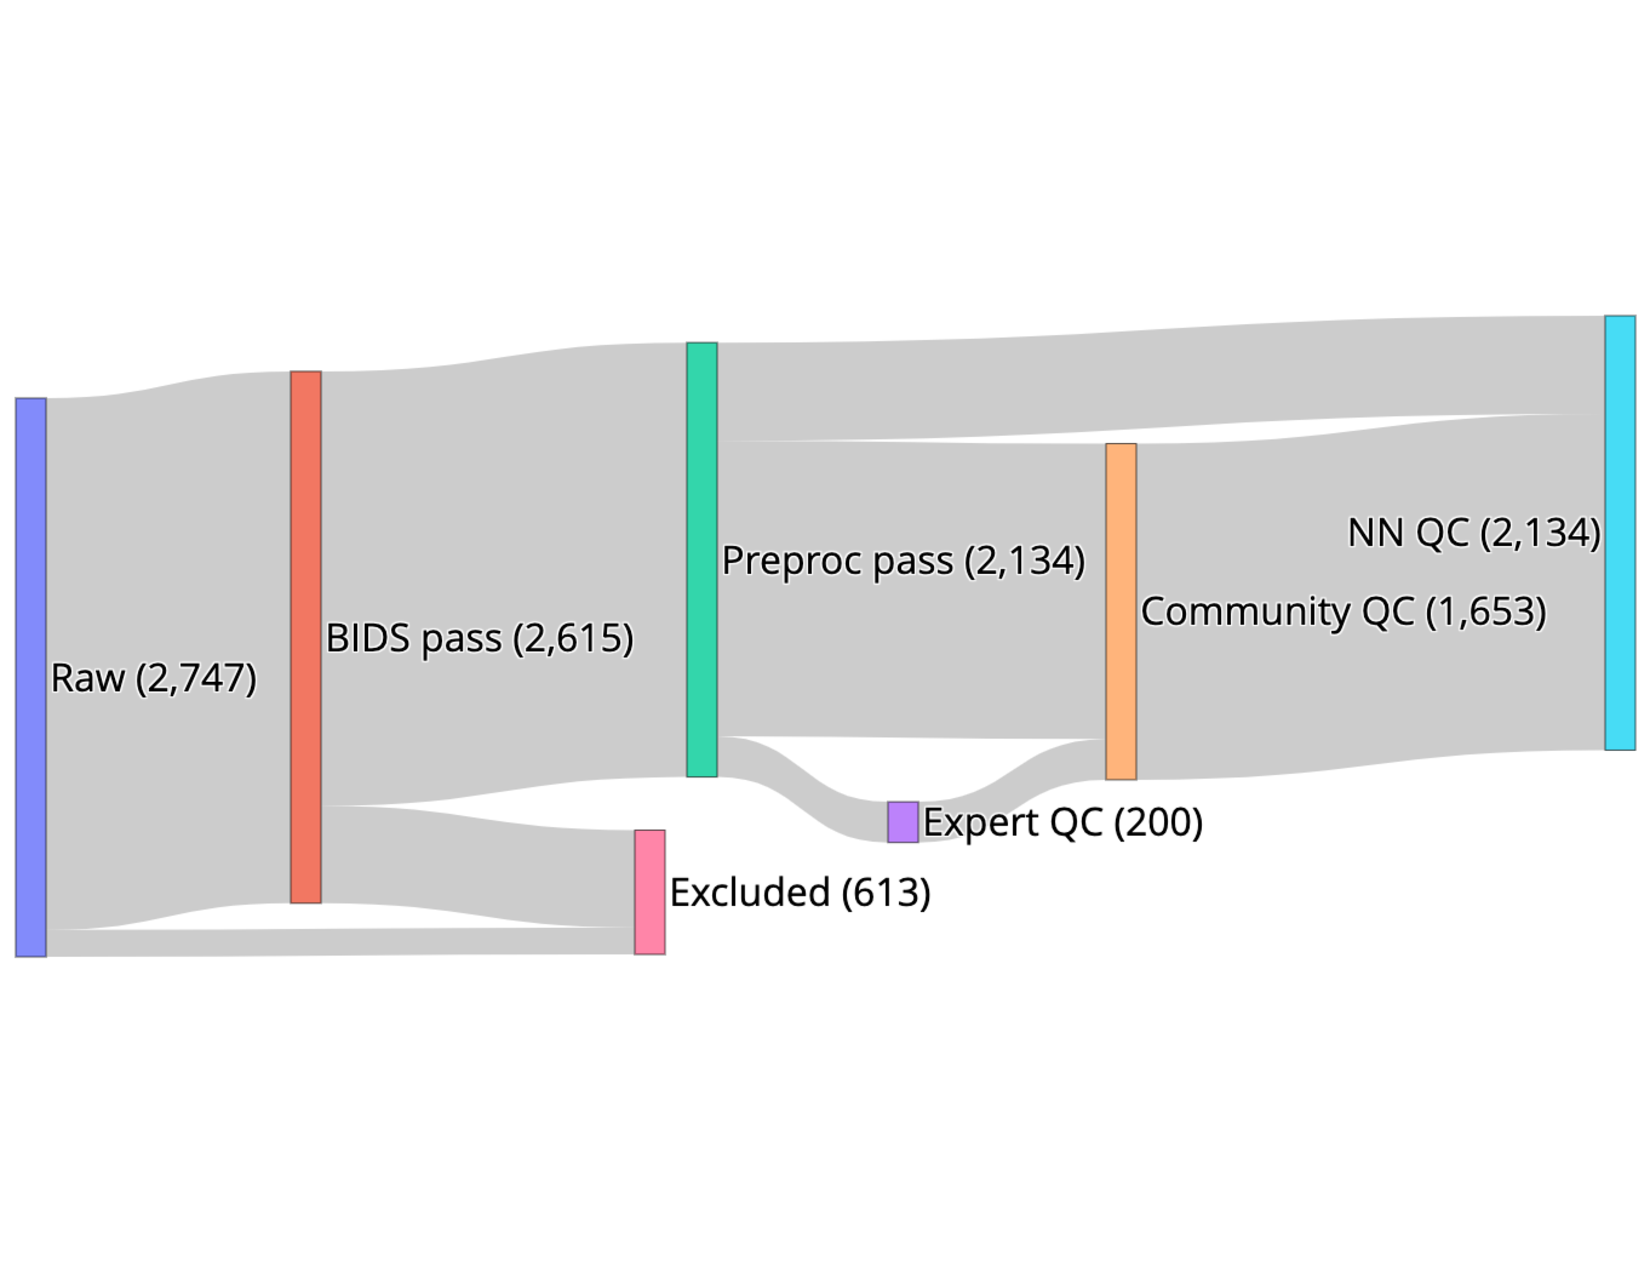
\includegraphics[width=0.75\linewidth]{hbn-pod2-sankey.pdf}
    \caption{%
        {\bf HBN-POD2 data provenance}:
        Imaging data for \num{2747} participants, aged 5-21 years and collected at four
        sites in the New York City area, was made available through the
        Functional Connectomes Project and the International Neuroimaging
        Data-Sharing Initiative (FCP-INDI).
        %
        These data were curated for compliance to the BIDS specification
        \cite{gorgolewski2016-lh} and availability of imaging metadata in json
        format. \num{2615} participants met this specification.
        %
        Imaging data was preprocessed using \emph{QSIPrep} \cite{cieslak2021-iq}
        to group, distortion correct, motion correct, denoise, coregister and
        resample MRI scans. Of the BIDS curated participants, \num{2134}
        passed this step, with the majority of failures coming from participants
        with missing dMRI scans.
        %
        Expert raters assigned QC scores to \num{200} of these participants,
        creating a ``gold standard'' QC subset (Figure \ref{fig:expert-qc}).
        Community raters then assigned
        binary QC ratings to a superset of the gold standard containing
        \num{1653} participants. An image classification algorithm was trained
        on a combination of automated quality metrics from \emph{QSIPrep} and community
        scientist reviews to ``extend'' the expert ratings to the community
        science subset (Figure \ref{fig:fibr-qc}.
        Finally, a deep learning QC model was trained on the
        community science subset to assign QC scores to the entire dataset and
        to future releases from HBN (Figure \ref{fig:dl-qc}).
        %
        The HBN-POD2 dataset, including QC ratings, is openly available through
        FCP-INDI.
    }
    \label{fig:hbn-sankey}
\end{figure}

\subsection*{Inputs}
%%%%%%%%%%%%%%%%%%%%%%%%%%%%%%%%%%%%%%%%

Inputs for this study consisted of MRI data from \added[comment=We added the input data release numbers as requested by Reviewer~\#2]{releases 1-9 of} the Healthy Brain Network
pediatric mental health study \replaced[comment=We added the source dataset citation at the editor's request.]{\cite{alexander2017yc, hbndata}}{\cite{alexander2017yc}}, containing dMRI data from
\num{2747} participants aged 5-21 years.
These data were measured using a \qty{1.5}{\tesla} Siemens mobile scanner on Staten Island (SI, $N=300$) and three fixed
\qty{3}{\tesla} Siemens MRI scanners at sites in the New York area: Rutgers
University Brain Imaging Center (RU, $N=873$), the CitiGroup Cornell Brain Imaging
Center (CBIC, $N=887$), and the City University of New York Advanced Science Research
Center (CUNY, $N=74$), where numbers in parentheses represent participant counts in HBN-POD2.
\added[comment=We added information about the ABCD-harmonized scan sequence in response to Reviewer \#2]{Site CBIC has two different acquisition types: one which shares its pulse sequence with sites RU and CUNY. In 19 CBIC subjects another acquisition protocol was used, which better matches the ABCD study diffusion protocol \cite{casey2018adolescent}.}
Informed consent was obtained from each participant aged 18 or
older. For participants younger than 18, written consent was obtained from their
legal guardians and written assent was obtained from the participant.
Voxel resolution was \qty{1.8}{\mm} $\times$ \qty{1.8}{\mm} $\times$ \qty{1.8}{\mm} with \num{64} non-colinear
directions measured for each \replaced[comment=We added clarifying text about different b-values for different scanning variants in response to Reviewer \#2]{
two degrees of diffusion weighting:
$b=1500$ \unit{\second \per \mm^{2}} and
$b=3000$ \unit{\second \per \mm^{2}} for the ABCD-harmonized sequence and
$b=1000$ \unit{\second \per \mm^{2}} and
$b=2000$ \unit{\second \per \mm^{2}} for the others.
}{
of $b=1000$ \unit{\second \per \mm^{2}} and
$b=2000$ \unit{\second \per \mm^{2}}.
}
Figure~\ref{fig:metric-dist} depicts the age distribution of study participants by sex for each of these scan sites as well as pairwise distributions for the automated quality metrics that are described in the next sections.

\subsection*{BIDS curation}
%%%%%%%%%%%%%%%%%%%%%%%%%%%%%%%%%%%%%%%%

We curated the imaging metadata for \num{2615} of the \num{2747} currently
available HBN participants. Using dcm2bids and custom scripts, we conformed the data
to the Brain Imaging Data Structure (BIDS)\cite{gorgolewski2016-lh}
specification. The BIDS-curated dataset is available on FCP-INDI and can be
accessed via AWS S3 at \url{s3://fcp-indi/data/Projects/HBN/BIDS_curated/}.

After conforming the data to BIDS, we used the ``Curation of BIDS'' (CuBIDS) package \cite{sydney-covitz2022-cubids} to identify unique combinations, or ``variants'' of imaging parameters in the curated dMRI and fieldmap acquisitions.
CuBIDS is a Python-based software package that provides a sanity-preserving workflow to help users reproducibly parse, validate, curate, and understand heterogeneous BIDS imaging datasets. CuBIDS includes a robust implementation of the BIDS Validator that scales to large samples and incorporates DataLad \cite{halchenko2021datalad}, a distributed data management system, to ensure reproducibility and provenance tracking throughout the curation process. CuBIDS tools also employ agglomerative clustering to identify variants of imaging parameters.
Each session was grouped according to metadata parameters that
affect the dMRI signal (PhaseEncodingDirection, EchoTime, VoxelSize, FlipAngle, PhasePartialFourier,
NumberOfVolumes, Fieldmap availability). We identified a total of 20 unique DWI acquisitions across
HBN-POD2, where about 5\% of acquisitions were different from the most common DWI acquisition at their
site.

\subsection*{Preprocessing}
%%%%%%%%%%%%%%%%%%%%%%%%%%%%%%%%%%%%%%%%

We performed dMRI preprocessing on \num{2615} participants, using \emph{QSIPrep}
\cite{cieslak2021-iq} 0.12.1, which is based on \emph{Nipype} 1.5.1
\cite{nipype1,nipype2}, RRID:SCR\_002502. \emph{QSIPrep} a robust and scalable
pipeline to group, distortion correct, motion correct, denoise, coregister and
resample MRI scans. In total, \num{417} participants failed this preprocessing
step, largely due to missing dMRI files. 
In keeping with the BIDS specification,
the preprocessed dataset is available as a derivative dataset within the
BIDS-curated dataset and can be access on AWS S3 at
\url{s3://fcp-indi/data/Projects/HBN/BIDS_curated/derivatives/qsiprep/}.
\emph{QSIPrep} fosters reproducibility by automatically generating thorough
methods boilerplate for later use in scientific publications, which we use for
the remainder of this subsection to document each preprocessing step.

\begin{itemize}

\item {\it Anatomical data preprocessing}
\replaced[comment=We amended the anatomical data preprocessing to account for that fact that some participants had multiple T1w images.]{
All T1-weighted (T1w) images found for each participant were corrected for intensity non-uniformity (INU)
using \texttt{N4BiasFieldCorrection} \cite{n4} (ANTs 2.3.1). If a single T1w was found, it was used as the T1w-reference throughout the workflow.
If multiple T1w images were found, a
T1w-reference map was computed after registration of the T1w images (after
INU-correction) using \texttt{mri\_robust\_template} \cite{fstemplate} (FreeSurfer 6.0.1).
}{
The T1-weighted (T1w) image was corrected for intensity non-uniformity (INU)
using \texttt{N4BiasFieldCorrection} \cite{n4} (ANTs 2.3.1), and used as
T1w-reference throughout the workflow.
}
The T1w-reference was then skull-stripped
using \texttt{antsBrainExtraction.sh} (ANTs 2.3.1), using OASIS as target
template. Spatial normalization to the ICBM 152 Nonlinear Asymmetrical template
version 2009c (RRID:SCR\_008796)\cite{mni} was performed through nonlinear
registration with \texttt{antsRegistration} (ANTs~2.3.1,
RRID:SCR\_004757)\cite{ants}, using brain-extracted versions of both T1w volume and
template. Brain tissue segmentation of cerebrospinal fluid (CSF), white-matter
(WM) and gray-matter (GM) was performed on the brain-extracted T1w using
\texttt{FAST} (FSL 6.0.3:b862cdd5, RRID:SCR\_002823)\cite{fsl-fast}.

\item {\it Diffusion data preprocessing}

Any images with a $b$-value less than \qty{100}{\second \per \mm^{2}} were treated
as a $b=0$ image. MP-PCA denoising as implemented in MRtrix3's \texttt{dwidenoise}~\cite{dwidenoise1} was applied with a 5-voxel window. After
MP-PCA, B1 field inhomogeneity was corrected using \texttt{dwibiascorrect} from
MRtrix3 with the N4 algorithm \cite{n4}. After B1 bias correction, the mean
intensity of the DWI series was adjusted so all the mean intensity of the $b=0$
images matched across each separate DWI scanning sequence.

FSL (version 6.0.3:b862cdd5)'s eddy was used for head motion correction
and Eddy current correction \cite{anderssoneddy}. Eddy was configured
with a \(q\)-space smoothing factor of 10, a total of 5 iterations, and
\num{1000} voxels used to estimate hyperparameters. A linear first level model
and a linear second level model were used to characterize Eddy
current-related spatial distortion. \(q\)-space coordinates were
forcefully assigned to shells. Field offset was attempted to be
separated from participant movement. Shells were aligned post-eddy. Eddy's
outlier replacement was run \cite{eddyrepol}. Data were grouped by
slice, only including values from slices determined to contain at least
\num{250} intracerebral voxels. Groups deviating by more than four standard
deviations from the prediction had their data replaced with imputed
values. Data was collected with reversed phase-encode blips, resulting
in pairs of images with distortions going in opposite directions. Here,
$b=0$ reference images with reversed phase encoding directions were used
along with an equal number of $b=0$ images extracted from the DWI scans.
From these pairs the susceptibility-induced off-resonance field was
estimated using a method similar to that described in \cite{topup}. The
fieldmaps were ultimately incorporated into the Eddy current and head
motion correction interpolation. Final interpolation was performed using
the \texttt{jac} method.

Several confounding time-series were calculated based on the
\emph{preprocessed DWI}: framewise displacement (FD) using the implementation
in \emph{Nipype} following the definitions by \cite{power-fd-dvars}. The DWI
time-series were resampled to ACPC, and their corresponding gradient directions
were rotated accordingly to generate a \emph{preprocessed DWI run
in ACPC space}. 

\end{itemize}

\noindent Many internal operations of \emph{QSIPrep} use \emph{Nilearn} 0.6.2
\cite{nilearn}, RRID:SCR\_001362 and \emph{DIPY} \cite{dipy}. For more details
of the pipeline, see
\href{https://qsiprep.readthedocs.io/en/latest/workflows.html}{the section
corresponding to workflows in \emph{QSIPrep}'s documentation}.

\subsection*{Cloud-based distributed preprocessing}
%%%%%%%%%%%%%%%%%%%%%%%%%%%%%%%%%%%%%%%%

The containerization of \emph{QSIPrep} provided a consistent preprocessing
pipeline for each participant but the number of participants made serial processing of
each participant prohibitive on a single machine. We used \emph{cloudknot}, a
previously developed cloud-computing library \cite{cloudknot} to
parallelize the preprocessing over individual participants on spot instances in the
Amazon Web Services Batch service. \emph{Cloudknot} takes as input a
user-defined Python function and creates the necessary AWS infrastructure to map
that function onto a range of inputs, in this case, the participant IDs.
Using \emph{cloudknot} and AWS Batch Spot Instances, the preprocessing cost less than \textdollar1.00 per participant.

\subsection*{Quality Control}
%%%%%%%%%%%%%%%%%%%%%%%%%%%%%%%%%%%%%%%%

To QC all available HBN dMRI data, we adopted a hybrid QC approach that
combines expert rating, community science, and deep learning, drawing on the
success of a previous application in assessing the quality of HBN's structural
T1w MRI data \cite{keshavan2019-er}. This method
\begin{enumerate*}[%
    label=(\roman*),%
    before={{ }},%
    itemjoin={{; }},%
    itemjoin*={{ and }}]
    \item starts with dMRI expert raters labelling a small subset of participants,
    the ``gold standard'' dataset
    \item amplifies these labels using a community science web application to
    extend expert ratings to a much larger subset of the data, the community
    science subset
    \item trains a deep learning model on the community science subset to
    predict expert decisions on the entire dataset.
\end{enumerate*}

\subsubsection*{Expert quality control}

The expert QC ``gold standard'' subset was created by randomly selecting 200
participants from the preprocessed dataset, sampled such that the proportional site
distribution in the gold standard subset matched that of the preprocessed
dataset.

We then developed \emph{dmriprep-viewer},
a dMRI data viewer and QC rating web application to display \emph{QSIPrep}
outputs and collect expert ratings \cite{richiehalford2022nirv}.
The viewer
ingests \emph{QSIPrep} outputs and generates a browser-based interface for
expert QC. It provides a study overview displaying the distributions of
\emph{QSIPrep}'s automated data quality metrics (described at
\url{https://qsiprep.readthedocs.io/en/latest/preprocessing.html#quality-control-data}).
Each datum on the study overview page is interactively linked to a participant-level
QC page that provides an interactive version of \emph{QSIPrep}'s visual reports
(described at
\url{https://qsiprep.readthedocs.io/en/latest/preprocessing.html#visual-reports}).
The viewer allows users to assign a rating of $-2$ (definitely fail), $-1$
(probably fail), $0$ (not sure), $1$ (probably pass), or $2$ (definitely pass) to a
participant.
To standardize rater expectations before rating, expert raters watched
a tutorial video (available on YouTube at \url{https://youtu.be/SQ0v-O-e5b8} and in the OSF project), \added[comment={In response to Reviewer~\#2 (point 1), we clarified that the video was used to specify a rating standard.}]{which demonstrated data for which each of these ratings was appropriate}.
Six of the
co-authors, who are all dMRI experts, rated the gold standard subset
using extensive visual examination of each participant's dMRI data,
including the preprocessed diffusion weighting imaging (DWI) time series, a plot of
motion parameters throughout the DWI scan, and full 3D volumes depicting
\begin{enumerate*}[%
    label=(\roman*),%
    before={{ }},%
    itemjoin={{, }},%
    itemjoin*={{ and }}]
    \item the brain mask and $b=0$ to T1w registration
    \item a directionally encoded color fractional anisotropy (DEC-FA) image laid over the $b=0$ volume.
\end{enumerate*}
See Appendix~\ref{fig:web-apps} for an example of the \emph{dmriprep-viewer} interface.

The distribution of scores given by the experts demonstrates that the
gold standard dataset included a range of data quality (Figure~\ref{fig:expert-qc:scatter:hist}). Mean expert ratings
correlated with the three \emph{QSIPrep} automated QC metrics that were most informative for the XGB model described in the next section:
neighboring DWI correlation \cite{yeh2019-kb} (Figure~\ref{fig:expert-qc:scatter:ndc}), maximum relative
translation (Figure~\ref{fig:expert-qc:scatter:translation}), and number of outlier slices (Figure~\ref{fig:expert-qc:scatter:outliers}). The neighboring DWI correlation characterizes
the pairwise spatial correlation between pairs of DWI volumes that sample
neighboring points in $q$-space. Since lower values indicate reduced data
quality, it is reassuring that the neighboring DWI correlation correlated directly with expert ratings
(Pearson CC: $0.797$). Conversely, high relative translation and a high number of
motion outlier slices reflect poor data quality and these metrics were inversely
related to mean expert rating (Pearson CC: $-0.692$ and Pearson CC: $-0.695$,
respectively).

In addition to agreeing qualitatively with \emph{QSIPrep}'s automated QC metrics
on average, the expert raters also tended to agree with each other (Figure~\ref{fig:expert-qc:irr}). We assessed
inter-rater reliability (IRR) using the pairwise Cohen's $\kappa$
\cite{di-eugenio2004-bb}, computed using the \emph{scikit-learn} \cite{scikit-learn} \texttt{cohen\_kappa\_score}
function with quadratic weights.
The pairwise $\kappa$ exceeded 0.52 in all cases, with a mean value of
0.648. In addition to the pairwise Cohen's $\kappa$, we also computed the
intra-class correlation (ICC) \cite{hallgren2012-ze} as a measure of IRR,
using the \emph{pingouin} statistical package \cite{vallat2018pingouin}
\texttt{intraclass\_corr} function.
ICC3k is the appropriate variant of the ICC to use when a fixed set of $k$ raters each
code an identical set of participants, as is the case here. ICC3k for inter-rater
reliability among the experts was 0.930 (95\% CI: [0.91, 0.94]), which is
qualitatively considered an ``excellent'' level of IRR \cite{Cicchetti1994-fz}.
The high IRR provides confidence that the average of the expert ratings for each
image in the gold standard is an appropriate target to use for training a
machine learning model that predicts the expert scores.

\begin{figure}[tbp]
    {\phantomsubcaption\label{fig:expert-qc:scatter:hist}}
    {\phantomsubcaption\label{fig:expert-qc:scatter:ndc}}
    {\phantomsubcaption\label{fig:expert-qc:scatter:translation}}
    {\phantomsubcaption\label{fig:expert-qc:scatter:outliers}}
    {\phantomsubcaption\label{fig:expert-qc:irr}}
    \centering
    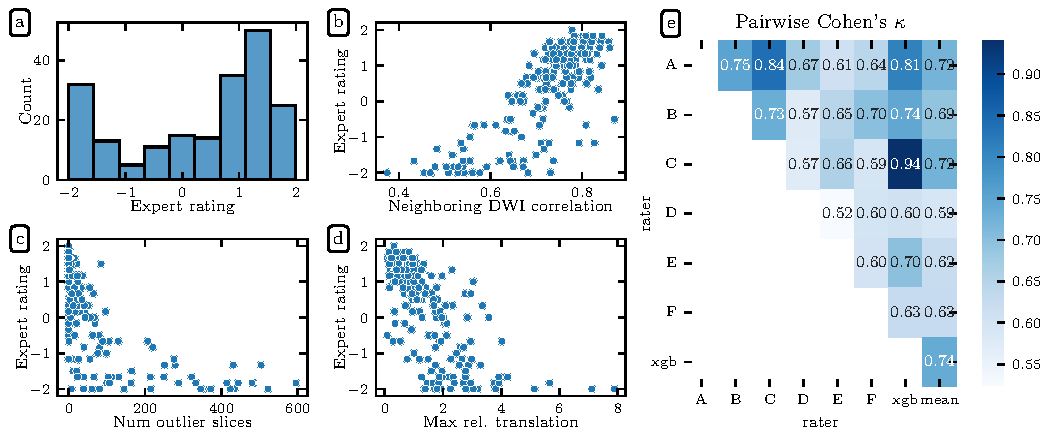
\includegraphics[width=\linewidth]{expert_qc.pdf}
    \caption{%
        {\bf Expert QC results}:
        Six dMRI experts rated a subset of \num{200} participants.  Experts agreed
        with \emph{QSIPrep}'s automated QC metrics.  Here we show the
        distribution of mean expert QC ratings \textbf{(a)} and associations
        between the mean expert QC rating and the \emph{QSIPrep} metrics
        \textbf{(b)} neighboring diffusion-weighted imaging (DWI) correlation 
        \cite{yeh2019-kb}, \textbf{(c)} maximum relative translation, and
        \textbf{(d)} number of outlier slices. As expected, neighboring DWI correlation is directly
        correlated with expert rating while the other two metrics are inversely
        correlated with expert rating.
        %
        \textbf{(e)} Experts agreed with each other. Here we show the pairwise
        Cohen's $\kappa$ measure of inter-rater reliability (see text for ICC
        calculations). The XGB model has an inter-rater reliability (quantified
        here as Cohen's $\kappa$) that is indistinguishable from the other
        raters
    }
    \label{fig:expert-qc}
\end{figure}

\subsubsection*{Community scientist quality control}

Although the expert raters achieved high IRR and yielded intuitive associations
with \emph{QSIPrep}'s automated QC metrics, generating expert QC labels for the
entire HBN-POD2 dataset would be prohibitively time consuming. To assess the
image quality of the remaining participants, we deployed \emph{Fibr}
(\url{https://fibr.dev}), a community science web application in which users
assigned binary pass/fail labels assessing the quality of horizontal slice DEC-FA
images overlaid on the $b=0$ image (see Figure~\ref{fig:web-apps} for an example).
Specifically, after a brief tutorial, \emph{Fibr} users saw individual
slices or an animated sequence of ten slices taken from the entire DEC-FA volume
that the expert raters saw. The \emph{Fibr} users, therefore, saw only a subset of
the imaging data that the dMRI experts had access to for a given participant, but they
saw data from many more participants. In total, \num{374} community scientists provided
\num{587778} ratings for a mean of $>50$ ratings per slice (or $>200$ ratings
per participant) from \num{1653} participants. Of the community scientists, \num{145}
raters provided $>3,000$ ratings each and are included in the \emph{Fibr} Community
Science Consortium as co-authors on this paper \cite{Ward-Fear2020-zq}.

\comment{This paragraph and Figure~\ref{fig:web-apps} were previously in an appendix. We have moved them to the main text at the editor's request.}
We created quality control web applications for both community raters and expert raters. These apps are publicly accessible at \url{https://fibr.dev} and at \url{http://www.nipreps.org/dmriprep-viewer/}, for the community science instrument and the expert rating instrument, respectively. We encourage readers to try these web applications on their own but have included screenshots and a summary of the interfaces in Figure~\ref{fig:web-apps}.

\begin{figure}[tbp]
    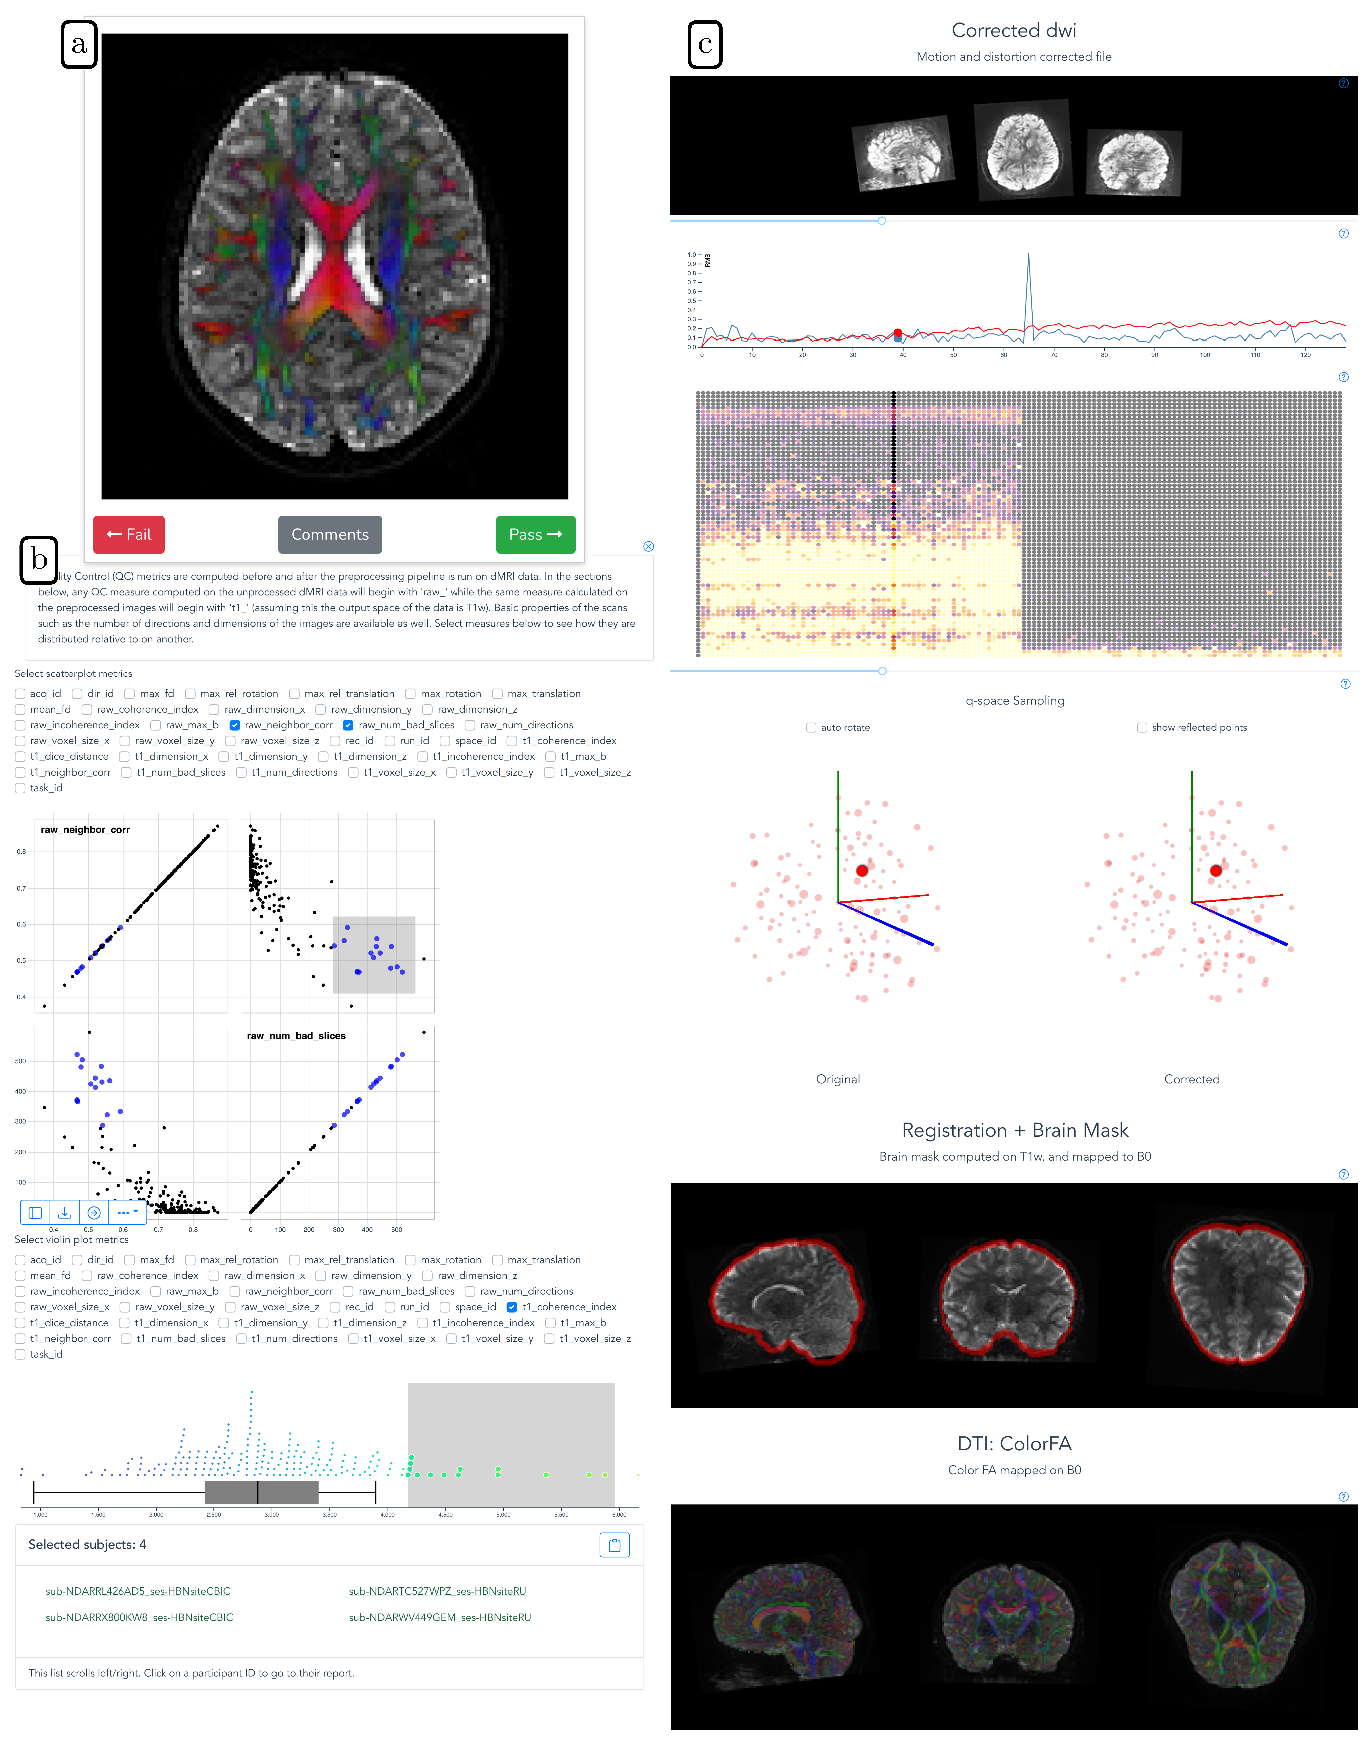
\includegraphics[width=0.9185\textwidth]{hbn-pod2-qc-instruments.pdf}
    \caption{
        {\bf HBN-POD2 quality control instruments}:
        {\bf (a)} The user interface for community science QC app \emph{Fibr}. After a
        tutorial, users are asked to give binary pass/fail ratings to
        each subject's DEC-FA image. The
        intuitive swipe or click interface allows community scientists to
        review more images than is practical for expert reviewers. Expert
        reviewers use the more advanced \emph{dmriprep-viewer} interface, where
        they can
        {\bf (b)} view the distribution of data quality metrics for the entire
        study using interactive scatterplots and violin plots, and
        {\bf (c)} inspect individual participants' preprocessing results,
        including corrected dMRI images, frame displacement, q-space
        sampling distributions, registration information, and a DTI
        model.
        \label{fig:web-apps}
    }
\end{figure}

There are three issues to account for when comparing \emph{Fibr} and expert QC ratings. First, the unadjusted \emph{Fibr} ratings were overly optimistic; i.e., on average,
community scientists were not as conservative as the expert raters
(Figure~\ref{fig:fibr-qc:scatter:fibr}). Second, different community scientists
provide data of differing accuracy. That is, they were less consistent across different views of the same image, and/or were less consistent with expert ratings for the same data). This means that data from some \emph{Fibr} raters was more informative than others. Third, important information
about data quality was provided in the \emph{QSIPrep} data quality metrics, which were not available to \emph{Fibr} raters. To account for rater
variability and take advantage of the information provided by \emph{QSIPrep},
we trained gradient boosted decision trees \cite{chen2016-eb} to predict expert scores, scaled to the range $[0, 1]$ and
binarized with a $0.5$ threshold,
based on a combination of community science ratings and 31 automated \emph{QSIPrep}
data quality metrics.
One can think of the gradient boosting model as assigning more weight to \emph{Fibr} raters who reliably agree with the expert raters, thereby resolving the aforesaid issues with community rater accuracy. We refer to this gradient boosting model as XGB.

\begin{figure}[tbp]
    {\phantomsubcaption\label{fig:fibr-qc:scatter:fibr}}
    {\phantomsubcaption\label{fig:fibr-qc:scatter:xgb}}
    {\phantomsubcaption\label{fig:fibr-qc:roc}}
    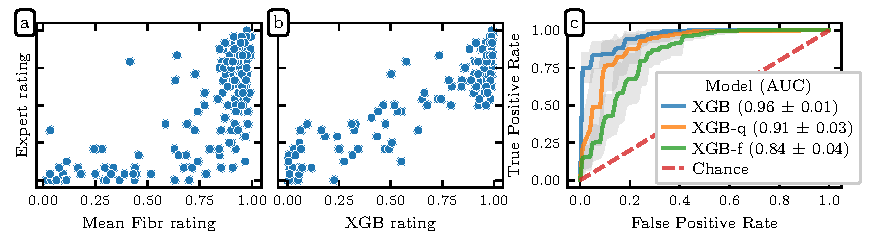
\includegraphics[width=\linewidth]{community_qc.pdf}
    \caption{%
        {\bf Community science predictions of the expert ratings}:
        Scatter plots showing the relationship between mean expert rating and
        both mean \emph{Fibr} rating \textbf{(a)} and XGB prediction
        \textbf{(b)}. \emph{Fibr} raters overestimated the quality of images
        compared to expert raters. But the XGB prediction compensated for this
        by incorporating automated QC metrics and weighting more valuable
        \emph{Fibr} raters.
        %
        \textbf{(c)} ROC curves for the XGB, XGB-q, and XGB-f models.
        Translucent bands represent one standard deviation from the mean
        of the cross-validation splits.
    }
    \label{fig:fibr-qc}
\end{figure}

All gradient boosting models were implemented as binary classifiers using the XGBoost library
\cite{xgboost}. The targets for these classifiers were the mean expert ratings
in the gold standard dataset, rescaled to the range $[0, 1]$ and binarized with
a threshold of $0.5$. Using repeated
stratified K-fold cross-validation, with three splits and two repeats, we
evaluated the models' performance in predicting the gold standard ratings. In
each fold, the best model hyperparameters were chosen using the scikit-optimize
\cite{scikit-optimize} \texttt{BayesSearchCV} class. 
Since each split resulted in a different XGB model and we required a single QC score
to train the deep learning model, we combined the models from each
cross-validation split using a voting classifier, computing a weighted averaged
of the predicted probability of passing from each model, weighted by its
out-of-sample ROC-AUC. This was implemented using scikit-learn's
\texttt{VotingClassifier} class.

To clarify the contributions of the automated QC metrics and the community
science raters, we trained two additional gradient boosting models
\begin{enumerate*}[%
    label=(\roman*),%
    before=\unskip{: },%
    itemjoin={{, }},%
    itemjoin*={{ and }}]
    \item one trained only on the automated \emph{QSIPrep} data quality metrics, which we
    call XGB-q
    \item one trained on only the \emph{Fibr} ratings, which we call XGB-f.
\end{enumerate*}
XGB-f may be viewed as a data-driven weighting of community scientists' ratings,
while XGB-q may be viewed as a generalization of data quality metric exclusion criteria.
XGB, combining information from both \emph{Fibr} ratings and \emph{QSIPrep} data quality
metrics attained a cross-validated area under the receiver operating curve
(ROC-AUC) of $0.96 \pm 0.01$ on the ``gold standard,'' where the $\pm$ indicates
the standard deviation of scores from repeated $k$-fold cross-validation
(Figure~\ref{fig:fibr-qc:scatter:xgb}). In contrast, XGB-q attained an ROC-AUC of
$0.91 \pm 0.03$ and XGB-f achieved an ROC-AUC of $0.84 \pm 0.04$.
The enhanced
performance of XGB-q over XGB-f shows that community scientists alone are not as
accurate as automated data quality metrics are at predicting expert ratings. And yet, the
increased performance of XGB over XGB-q demonstrates that there is additional
image quality information to be gained by incorporating community scientist input.

\comment{This paragraph and Tables~\ref{tab:xgb-shap} and~\ref{tab:xgb-q-shap} were previously in an appendix. We have moved them to the main text at the editor's request.}
We used SHapley Additive exPlanations (SHAP) to measure the global feature importance of the automated quality metrics in the gradient boosting models.
SHAP is a method to explain individual predictions based on game theoretically optimal Shapley values \cite{lundberg2017unified}. To estimate global feature importance for the XGB and XGB-q models, we use the \texttt{shap} library's \texttt{TreeExplainer} \cite{lundberg2020local} and average the absolute Shapley value per feature across each individual prediction. Tables~\ref{tab:xgb-shap} and \ref{tab:xgb-q-shap} list the \emph{QSIPrep} automated QC metric features in order of decreasing mean absolute shap value for the XGB and XGB-q models, respectively. We chose the top three metrics from Table~\ref{tab:xgb-shap} to plot metric distributions in Figure~\ref{fig:metric-dist} and correlations with the expert QC results in Figure~\ref{fig:expert-qc}.

\begin{table}[tbp]
\begin{multicols}{2}
\centering
\begin{tabular}{lr}
\toprule
{} &  mean abs shap \\
feature               &                           \\
\midrule
raw\_neighbor\_corr     &                  0.666429 \\
max\_rel\_translation   &                  0.348662 \\
raw\_num\_bad\_slices    &                  0.288937 \\
t1\_neighbor\_corr      &                  0.282198 \\
raw\_incoherence\_index &                  0.229733 \\
raw\_coherence\_index   &                  0.162103 \\
max\_rel\_rotation      &                  0.118963 \\
mean\_fd               &                  0.116457 \\
max\_fd                &                  0.099359 \\
max\_rotation          &                  0.078774 \\
t1\_coherence\_index    &                  0.035553 \\
t1\_dice\_distance      &                  0.034510 \\
max\_translation       &                  0.032323 \\
t1\_incoherence\_index  &                  0.030225 \\
raw\_voxel\_size\_x      &                  0.000000 \\
raw\_voxel\_size\_y      &                  0.000000 \\
raw\_voxel\_size\_z      &                  0.000000 \\
raw\_num\_directions    &                  0.000000 \\
raw\_max\_b             &                  0.000000 \\
raw\_dimension\_y       &                  0.000000 \\
raw\_dimension\_z       &                  0.000000 \\
t1\_voxel\_size\_x       &                  0.000000 \\
t1\_dimension\_x        &                  0.000000 \\
t1\_dimension\_y        &                  0.000000 \\
t1\_dimension\_z        &                  0.000000 \\
t1\_voxel\_size\_y       &                  0.000000 \\
t1\_voxel\_size\_z       &                  0.000000 \\
t1\_max\_b              &                  0.000000 \\
t1\_num\_bad\_slices     &                  0.000000 \\
t1\_num\_directions     &                  0.000000 \\
raw\_dimension\_x       &                  0.000000 \\
\bottomrule
\end{tabular}
\captionof{table}{%
  XGB mean absolute shap values
  \label{tab:xgb-shap}
}

{\nolinenumbers
\begin{tabular}{lr}
\toprule
{} &  mean abs shap \\
feature               &                           \\
\midrule
raw\_neighbor\_corr     &                  0.767536 \\
raw\_incoherence\_index &                  0.453897 \\
raw\_num\_bad\_slices    &                  0.430422 \\
t1\_coherence\_index    &                  0.382218 \\
max\_rel\_translation   &                  0.363052 \\
raw\_coherence\_index   &                  0.320438 \\
t1\_neighbor\_corr      &                  0.250948 \\
t1\_dice\_distance      &                  0.248104 \\
t1\_incoherence\_index  &                  0.242348 \\
max\_rel\_rotation      &                  0.135590 \\
mean\_fd               &                  0.128642 \\
max\_translation       &                  0.120815 \\
max\_fd                &                  0.119739 \\
max\_rotation          &                  0.101209 \\
t1\_num\_bad\_slices     &                  0.007075 \\
raw\_dimension\_y       &                  0.000000 \\
raw\_dimension\_z       &                  0.000000 \\
raw\_voxel\_size\_x      &                  0.000000 \\
raw\_voxel\_size\_y      &                  0.000000 \\
raw\_voxel\_size\_z      &                  0.000000 \\
raw\_max\_b             &                  0.000000 \\
t1\_voxel\_size\_x       &                  0.000000 \\
raw\_num\_directions    &                  0.000000 \\
t1\_dimension\_x        &                  0.000000 \\
t1\_dimension\_y        &                  0.000000 \\
t1\_dimension\_z        &                  0.000000 \\
t1\_voxel\_size\_y       &                  0.000000 \\
t1\_voxel\_size\_z       &                  0.000000 \\
t1\_max\_b              &                  0.000000 \\
t1\_num\_directions     &                  0.000000 \\
raw\_dimension\_x       &                  0.000000 \\
\bottomrule
\end{tabular}
\captionof{table}{%
  XGB-q mean absolute shap values
  \label{tab:xgb-q-shap}
}
}
\end{multicols}
\end{table}


As a way of evaluating the quality of the XGB predictions, consider the fact
that the average Cohen's $\kappa$ between XGB and the expert raters was 0.74,
which is higher than the average Cohen's $\kappa$ between any of the other raters
and their human peers (Figure~\ref{fig:expert-qc}). This is not surprising,
given that the XGB model was fit to optimize this match, but further
demonstrates the goodness of fit of this model.

Nevertheless, this provides confidence in using the XGB scores in the next step of analysis, where we treat the XGB model as an additional coder and extend XGB ratings to participants without \emph{Fibr} ratings.
In this case, when a subset of participants is coded by multiple raters and the
reliability of their ratings is meant to generalize to other participants rated by
only one coder, the single-measure ICC3, as opposed to ICC3k, should be used. When adding XGB to the
existing expert raters as a seventh expert, we achieved
$\textbf{ICC3} = 0.709 (95\% CI: [0.66, 0.75])$. 
The high ICC3 value after inclusion of the XGB model justifies using the XGB scores as the target for training an image-based deep learning
network.

\subsubsection*{Automated quality control labelling through deep learning}

While the XGB ``rater'' does a good job of extending QC ratings to the entire
community science subset, this approach requires \emph{Fibr} scores; without community
science \emph{Fibr} scores, only the less accurate XGB-q
prediction can be employed. Consequently, a new, fully automated QC approach is needed that can be readily applied to future data releases from HBN.

We therefore trained deep convolutional neural networks to predict binarized XGB ratings directly from \emph{QSIPrep} outputs.
We modified an existing 3D convolutional neural network (CNN) architecture \cite{zunair2020-bs}---previously
applied to the ImageCLEF Tuberculosis Severity Assessment 2019 benchmark \cite{dicente2019clef}---to accept multichannel input generated from the preprocessed dMRI:
the $b=0$ reference diffusion image, each of the three
cardinal axis components of the DEC-FA image, and, optionally, automated QC
metrics from \emph{QSIPrep}. We trained these networks on XGB scores and validated it
against the gold standard expert-scored dataset. We refer to the convolutional
neural network model trained only on imaging data as CNN-i and the model that
incorporates automated QC metrics as CNN-i+q.

\comment{These two paragraphs and Figures~\ref{fig:dl-architecture} and~\ref{fig:dl-loss} were previously in an appendix. We have moved them to the main text at the editor's request.}
Both the CNN-i and CNN-i+q models were implemented in Tensorflow 2 \cite{tensorflow} using the Keras module \cite{keras}.
The image processing part of the model architecture was
identical for both models: a modification of an existing 3D CNN
\cite{zunair2020-bs} previously applied to assess tuberculosis severity
\cite{dicente2019clef}. It accepts a 3D volume as input with four channels
\begin{enumerate*}[%
    label=(\roman*),%
    before=\unskip{: },%
    itemjoin={{, }},%
    itemjoin*={{ and }}]
    \item the $b=0$ reference volume
    \item DEC-FA in the $x$-direction
    \item DEC-FA in the $y$-direction
    \item DEC-FA in the $z$-direction.
\end{enumerate*}
The \emph{QSIPrep}'s automated QC metrics were included as an additional fifth
channel. The CNN-i+q model architecture is summarized in
Figure~\ref{fig:dl-architecture}. Upon input, the CNN-i+q model extracts the
imaging channels and passes them through the CNN architecture. The remaining data quality
metrics channel is flattened and passed ``around'' the CNN architecture and
concatenated with the output of the convolutional layers. This concatenated
output is then passed through a fully-connected layer to produce a single
output, the probability of passing QC. This architecture has \num{1438783} trainable
parameters.

\begin{figure}[tbp]
    \centering
    {\phantomsubcaption\label{fig:dl-architecture:complete}}
    {\phantomsubcaption\label{fig:dl-architecture:cnn}}
    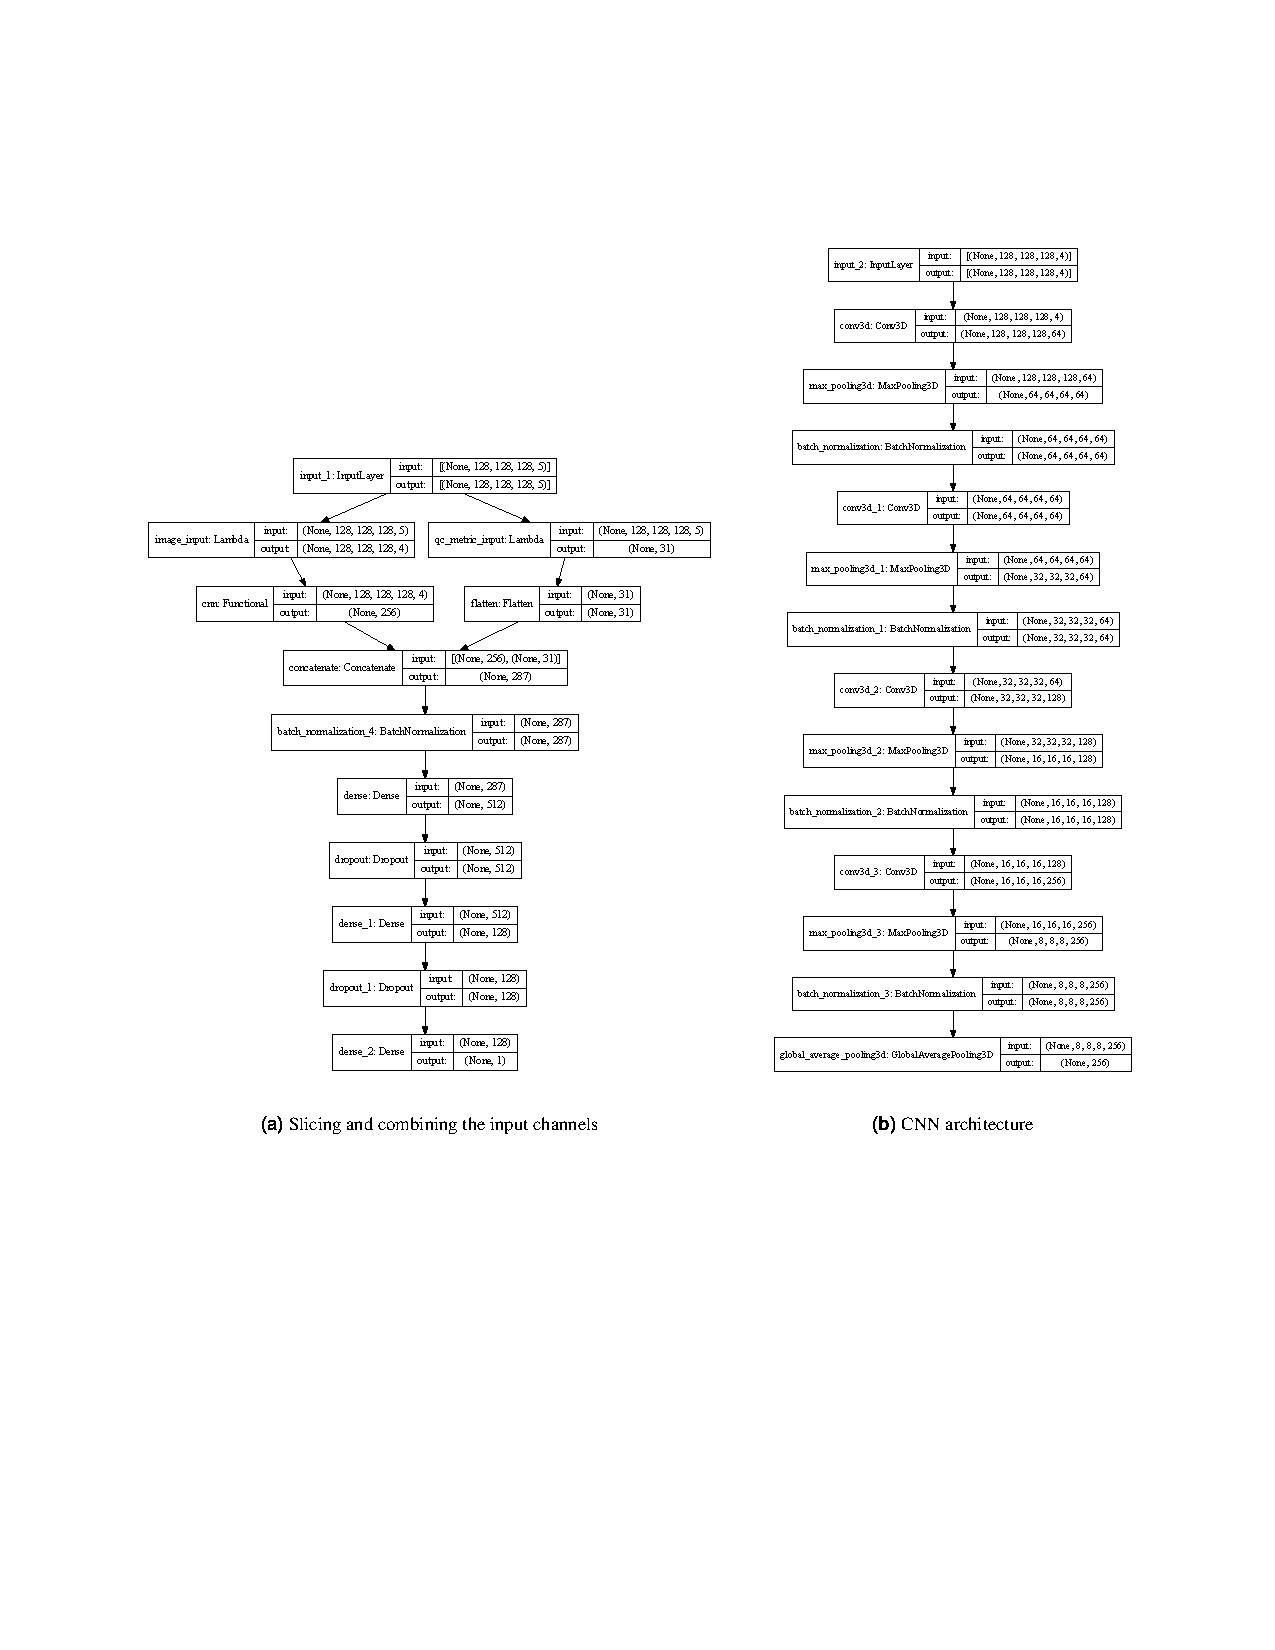
\includegraphics[width=\linewidth]{model_combined.pdf}
    \caption{%
        {\bf Deep learning model architecture}:
        \textbf{(a)} The CNN-i+q model accepts multichannel input that combined
        four imaging channels with a fifth channel containing 31 \emph{QSIPrep}
        automated data quality metrics. The imaging channels are separated from the data quality
        channel using \texttt{Lambda} layers. The imaging channels are passed
        through a CNN \textbf{(b)}, the output of which is concatenated with the
        data quality metrics, batch normalized and passed through two fully-connected (FC)
        layers, with rectified linear unit (ReLu) activation functions and with
        512 and 128 units respectively. Each FC layer is followed by a dropout
        layer which drops 40\% of the input units. The final layer contains a
        single unit with a sigmoid activation function and outputs the
        probability of passing QC.
        %
        \textbf{(b)} The CNN portion of the model passes the imaging input
        through four convolutional blocks. Each block consists of a 3D
        convolutional layer with a kernel size of 3 and a ReLu activation, a 3D
        max pooling layer with a pool size of 2, and a batch normalization layer
        with Tensorflow's default parameters. The number of filters in the
        convolutional layers in each block are 64, 64, 128, and 256 respectively.
        The output of the final block is passed through a 3D global average
        pooling layer with Tensorflow's default parameters.
    }
    \label{fig:dl-architecture}
\end{figure}

To estimate the variability in model training, we trained ten separate models using
different training and validation splits of the data. The gold standard dataset
was not included in any of these splits and was reserved for reporting final
model performance. Models were optimized for binary crossentropy loss using the
Adam optimizer \cite{kingma2017adam} with an initial learning rate of 0.0001. We
reduced the learning rate by a factor of 0.5 when the validation loss plateaued
for more than two epochs. We also stopped training when the validation loss
failed to improve by more than 0.001 for twenty consecutive epochs. These two
adjustments were made using the \texttt{ReduceLROnPlateau} and
\texttt{EarlyStopping} callbacks in Tensorflow 2 \cite{tensorflow} respectively.
The training and validation loss curves for both the CNN-i and CNN-i+q models
are depicted in Figure~\ref{fig:dl-loss}. While the CNN-i+q model achieved
better validation loss, it did not outperform the CNN-i model on the held out
gold standard dataset.

\begin{figure}[tbp]
    \centering
    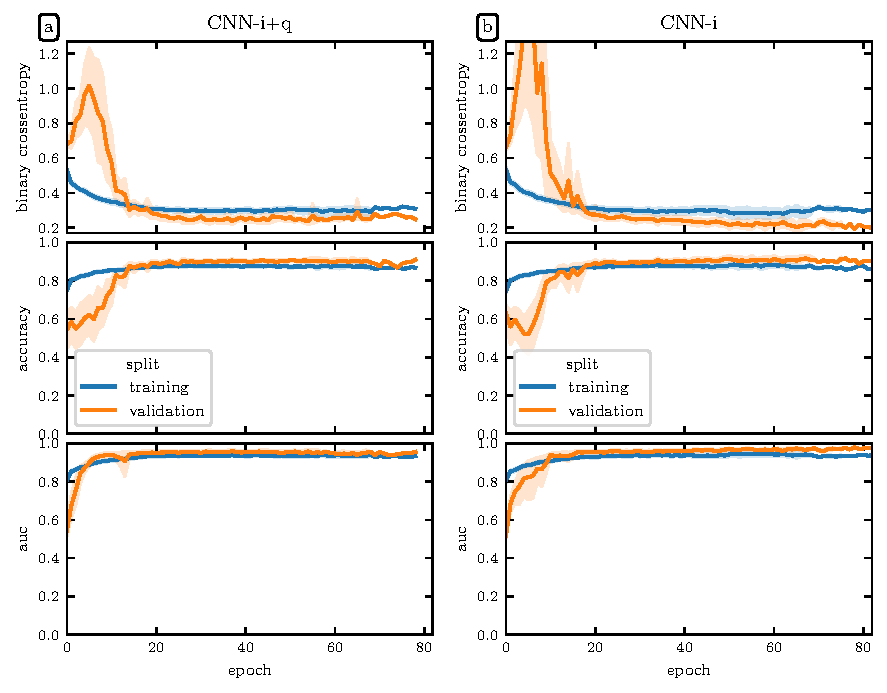
\includegraphics[width=\linewidth]{dl_learning_curves.pdf}
    \caption[Deep learning model loss curves]{%
        {\bf Deep learning model loss curves}:
        The binary cross-entropy loss (top), accuracy (middle), and ROC-AUC
        (bottom) for \textbf{(a)} the CNN-i+q model and \textbf{(a)} the CNN-i
        model. Model performance typically plateaued after twenty epochs but was
        allowed continue until meeting the early stopping criterion. The error
        bands represent a bootstrapped 95\% confidence interval.
    }
    \label{fig:dl-loss}
\end{figure}

The two models performed nearly identically and achieved an ROC-AUC of $0.947 \pm 0.004$ (Figure~\ref{fig:dl-qc:roc}). The
near-identical performance suggests that \emph{QSIPrep}'s automated data quality metrics
provided information that was redundant with information available in the imaging
data. Both CNN-i and CNN-i+q outperformed XGB-q, which was trained only on
automated QC metrics, but both modestly underperformed relative to the full XGB model,
that uses \emph{Fibr} scores in addition to the \emph{QSIPrep} data quality metrics.

\begin{figure}[!t]
    {\phantomsubcaption\label{fig:dl-qc:roc}}
    {\phantomsubcaption\label{fig:dl-qc:joint}}
    {\phantomsubcaption\label{fig:dl-qc:hist:sex}}
    {\phantomsubcaption\label{fig:dl-qc:hist:site}}
    \centering
    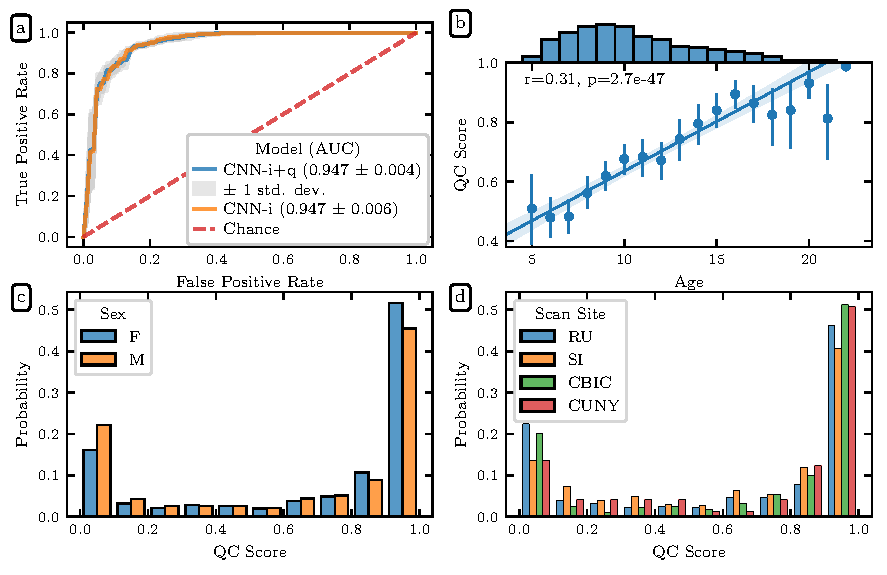
\includegraphics[width=\linewidth]{deep_learning_qc.pdf}
    \caption{%
        {\bf Deep learning QC scores}:
        \textbf{(a)} ROC curves for two deep learning models trained on imaging data: one trained with
        additional automated data quality metrics from \emph{QSIPrep} (blue) and one
        trained without (orange). The models performed roughly identically,
        reflecting that the data quality metrics are derived from the imaging data and are therefore redundant. Both outperformed the XGB-q predictions, indicating the
        added value of the diffusion weighted images. However, both models
        underperformed the XGB predictions, which also incorporate
        information from \emph{Fibr} ratings for each scan. The error bands
        represent one standard deviation from the mean of the cross-validation
        splits.
        %
        \textbf{(b)} Joint distributions showing a strong direct association
        between age and QC score (Pearson CC: $0.31$). This likely reflects the well-known negative
        association between age and head motion in pediatric neuroimaging.
        The dots encode the mean QC score for each year of age with error bands
        representing a bootstrapped 95\% confidence interval. The line depicts
        a linear regression relating age and QC score with translucent bands
        encoding a bootstrapped 95\% confidence interval.
        %
        Histograms showing the relationship between participants QC scores and
        their sex \textbf{(c)} and scan site \textbf{(d)}. QC distributions are independent
        of sex and scanning site.
    }
    \label{fig:dl-qc}
\end{figure}

The openly available HBN-POD2 data released with this paper provides four QC ratings: the mean expert QC ratings, XGB-q and
XGB predicted scores, as well as the CNN-i predicted score. However, we treat the CNN-i
score as the definitive QC score because it is available for all participants,
can be easily calculated for new participants in future HBN releases, and is more
accurate than XGB-q in predicting expert ratings in the ``gold standard'' report set. When we refer to a participant's QC score without
specifying a generating model, the CNN-i score is assumed.
Figure~\ref{fig:dl-qc} depicts the distribution of these QC scores by age
(Figure~\ref{fig:dl-qc:joint}), sex (Figure~\ref{fig:dl-qc:hist:sex}), and scanning site
(Figure~\ref{fig:dl-qc:hist:site}). QC distributions are similar for each scan site
and for male and female participants. Responses for the sex variable in HBN phenotypic data are limited to ``male'' and ``female.''

\subsubsection*{Tractometry}

To further validate the importance of quality control, we used tract profiling \cite{yeatman2012-rc,jones2005pasta,colby2012along,odonnell2009tract, kruper2021evaluating}, which is a subset of tractometry \cite{jones2005pasta,bells2011tractometry}. In particular, tract profiling uses the results of dMRI tractography to quantify properties of the white matter along major pathways. We used the Python Automated Fiber Quantification toolbox (pyAFQ) as previously described \cite{kruper2021evaluating}. Briefly, probabilistic tractography was performed using constrained spherical deconvolution fiber orientation distribution functions \cite{tournier2008csd}, as implemented in DIPY \cite{dipy}. Twenty-four major tracts, which are enumerated in Figure~\ref{fig:qc-profiles:md}, were identified using multiple criteria: inclusion ROIs and exclusion ROIs \cite{Wakana2007-nw}, combined with a probabilistic atlas \cite{Hua2008-di}. Each streamline was resampled to 100 nodes and the robust mean at each location was calculated by estimating the 3D covariance of the location of each node and excluding streamlines that are more than 5 standard deviations from the mean location in any node. Finally, a bundle profile of tissue properties in each bundle was created by interpolating the value of MRI maps of these tissue properties to the location of the nodes of the resampled streamlines designated to each bundle. In each of 100 nodes, the values were summed across streamlines, weighting the contribution of each streamline by the inverse of the Mahalanobis distance of the node from the average of that node across streamlines. Bundle profiles of mean diffusivity (MD) and fractional anisotropy (FA) from the diffusional kurtosis imaging (DKI) model \cite{jensen2005-ta}, implemented in DIPY \cite{Henriques2021-lk}, were used in technical validation of the data and evaluation of the impacts of QC.
We used the previously mentioned \emph{cloudknot} cloud-computing library \cite{cloudknot} to parallelize the pyAFQ tractometry pipeline over individual participants on spot instances in the
Amazon Web Services Batch service.

\comment{This paragraph and Figures~\ref{fig:qc-profiles:md} and~\ref{fig:qc-profiles:fa} were previously in an appendix. We have moved them to the main text at the editor's request.}
Here, we plot mean diffusivity tract profiles (MD, Figure~\ref{fig:qc-profiles:md}) and fractional anisotropy profiles (FA, Figure~\ref{fig:qc-profiles:fa}) grouped
into four QC bins along the length of twenty-four bundles. While some bundles,
such as the cingulum cingulate (CGC) and the inferior longitudinal fasciculus
(ILF), appear insensitive to QC score, others, such as the uncinate (UNC) and
the orbital portion of the corpus callosum, exhibit strong differences between
QC bins. In most bundles, low QC scores tend to flatten the MD profile, indicating that MD appears artifactually homogeneous across the bundle.

\begin{figure}[tbp]
    \centering
    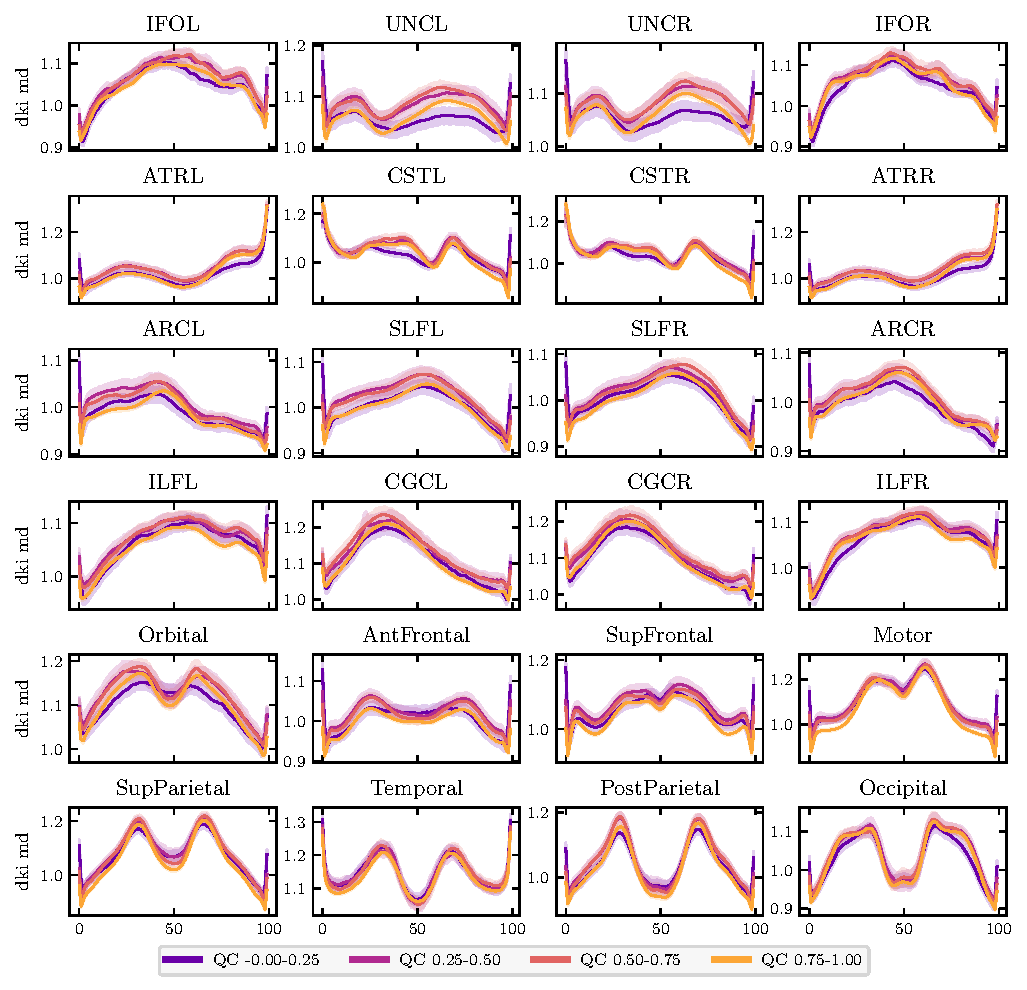
\includegraphics[width=\linewidth]{qc-bins-dki-md.pdf}
    \caption{%
        {\bf MD bundle profiles show large QC group differences}:
        MD profiles binned by QC score in twenty-four major while matter
        bundles.  The $x$-axis represents distance along the length of the fiber
        bundle.
        %
        The left and right uncinate bundles were the most sensitive
        to QC score. Generally, QC score tended to flatten bundle profiles.
        %
        Error bands represent bootstrapped 95\% confidence intervals. Bundle
        abbreviations for lateralized bundles contain a trailing ``L'' or ``R''
        indicating the hemisphere. Bundle abbreviations:
        inferior fronto-occipital fasciculus (IFO),
        uncinate (UNC),
        thalamic radiation (ATR),
        corticospinal (CST),
        arcuate (ARC),
        superior longitudinal fasciculus (SLF).
        inferior longitudinal fasciculus (ILF),
        cingulum cingulate (CGC),
        orbital corpus callosum (Orbital),
        anterior frontal corpus callosum (AntFrontal),
        superior frontal corpus callosum (SupFrontal),
        motor corpus callosum (Motor),
        superior parietal corpus callosum (SupParietal),
        temporal corpus callosum (Temporal),
        post-parietal corpus callosum (PostParietal), and
        occipital corpus callosum (Occipital).
    }
    \label{fig:qc-profiles:md}
\end{figure}
\begin{figure}[tbp]
    \centering
    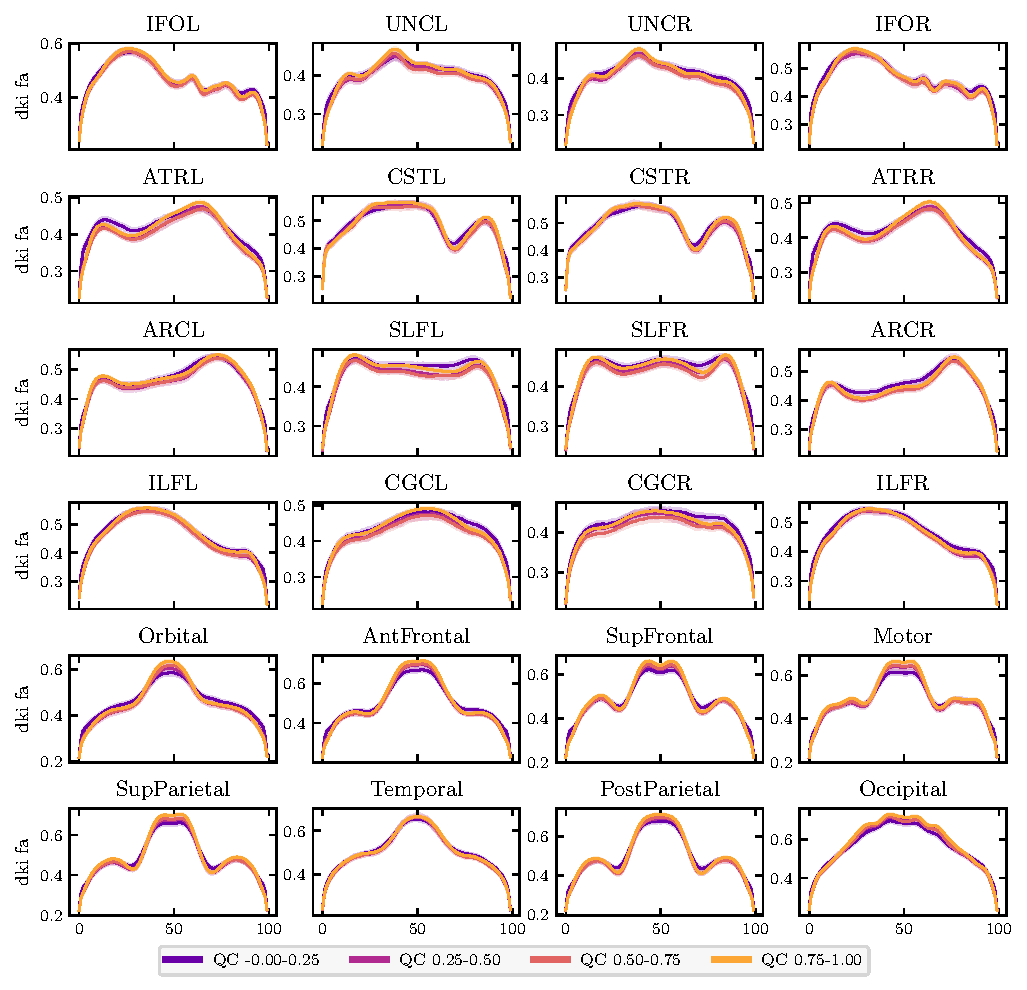
\includegraphics[width=\linewidth]{qc-bins-dki-fa.pdf}
    \caption[FA bundle profiles]{%
        {\bf FA bundle profiles binned by QC score}:
        FA profiles binned by QC score in twenty-four major while matter
        bundles. The $x$-axis represents distance along the length of the fiber
        bundle. Error bands represent bootstrapped 95\% confidence intervals.
        Bundle abbreviations are as in Figure~\ref{fig:qc-profiles:md}
    }
    \label{fig:qc-profiles:fa}
\end{figure}

%%%%%%%%%%%%%%%%%%%%%%%%%%%%%%%%%%%%%%%%%%%%%%%%%%%%%%%%%%%%
\section*{Data Records}
%%%%%%%%%%%%%%%%%%%%%%%%%%%%%%%%%%%%%%%%%%%%%%%%%%%%%%%%%%%%

\subsection*{Curated imaging data}
%%%%%%%%%%%%%%%%%%%%%%%%%%%%%%%%%%%%%%%%

Curated BIDS data and their corresponding \emph{QSIPrep} outputs are public resources that can be accessed by anyone using DataLad\cite{datalad} or standard Amazon Simple Storage Service (S3) access tools. The curated data are available in the FCP-INDI S3 bucket and as a DataLad dataset\cite{hbnpod2data} as indicated in Table~\ref{tab:data-records}.
Likewise, the \emph{QSIPrep} derivatives are available on FCP-INDI, as a standalone DataLad dataset\cite{hbnpod2qsiprepdata}, and as a derivative subdataset in the primary HBN-POD2 DataLad dataset\cite{hbnpod2data}.
These processed diffusion derivatives are \href{
https://qsiprep.readthedocs.io/en/latest/preprocessing.html#outputs-of-qsiprep}{
standard \emph{QSIPrep} outputs}, which contain preprocessed imaging data
along with the corresponding QC metrics:

\begin{itemize}
    \item \emph{Anatomical Data} Preprocessed images, segmentations and transforms for spatial normalization are located in the \texttt{anat/} directory of each session. The gray matter, white matter and  cerebrospinal fluid (\texttt{GM}, \texttt{WM}, \texttt{CSF}) probabilistic segmentations are provided in nifti format with the \texttt{\_probtissue} suffix. The deterministic  segmentation is in \texttt{\_dseg.nii.gz}. All images are in alignment with AC-PC-aligned  \texttt{sub-X\_desc-preproc\_T1w.nii.gz} image unless they have \texttt{space-MNI152NLin2009cAsym} in their file name, in which case they are aligned to the MNI Nonlinear T1-weighted asymmetric brain template (version 2009c)\cite{Fonov2009-ze}. The spatial transform between the AC-PC T1w image and MNI space is in the ITK/ANTs format file named \texttt{sub-X\_from-MNI152NLin2009cAsym\_to-T1w\_mode-image\_xfm.h5}. The brain mask from \texttt{ANTsBrainExtraction.sh} is included in the file with the \texttt{\_desc-brain\_mask.nii.gz} suffix.

    \item \emph{Diffusion Data} The preprocessed dMRI scan and accompanying metadata are in the  \texttt{dwi} directory of each session. The fully-preprocessed dMRI data is follows the naming pattern \texttt{sub-X\_space-T1w\_desc-preproc\_dwi.nii.gz}. These images all have an isotropic voxel size of \qty{1.7}{\mm} and are aligned in world coordinates with the anatomical image located at \texttt{anat/sub-X\_desc-preproc\_T1w.nii.gz}. Gradient information is provided in \texttt{bval/bvec} format compatible with DIPY and DSI Studio and the \texttt{.b} format compatible with MRtrix3. Volume-wise QC metrics including head motion parameters are included in the \texttt{confounds.tsv} file. Automatically computed quality measures for the entire image series are provided in the \texttt{ImageQC.csv} file, which includes the neighboring DWI Correlation, number of bad slices and head motion summary statistics.
    Figure~\ref{fig:metric-dist} depicts pairwise distributions for the three of these automated data quality metrics that were most informative in QC models described later
    \replaced[comment={We changed this reference from an appendix to tables in the main text.}]{
    (see Tables~\ref{tab:xgb-shap} and~\ref{tab:xgb-q-shap}).
    }{
    (see Appendix~?? for further details).
    }
    The \texttt{desc-brain\_mask} file is a dMRI-based brain mask that should only be used when the T1w-based brain mask is inappropriate (i.e. when no susceptibility distortion correction has been applied).
\end{itemize}

\begin{figure}[tbp]
    {\phantomsubcaption\label{fig:metric-dist:age}}
    {\phantomsubcaption\label{fig:metric-dist:ndc-slices}}
    {\phantomsubcaption\label{fig:metric-dist:ndc-translation}}
    {\phantomsubcaption\label{fig:metric-dist:slices-translation}}
    \centering
    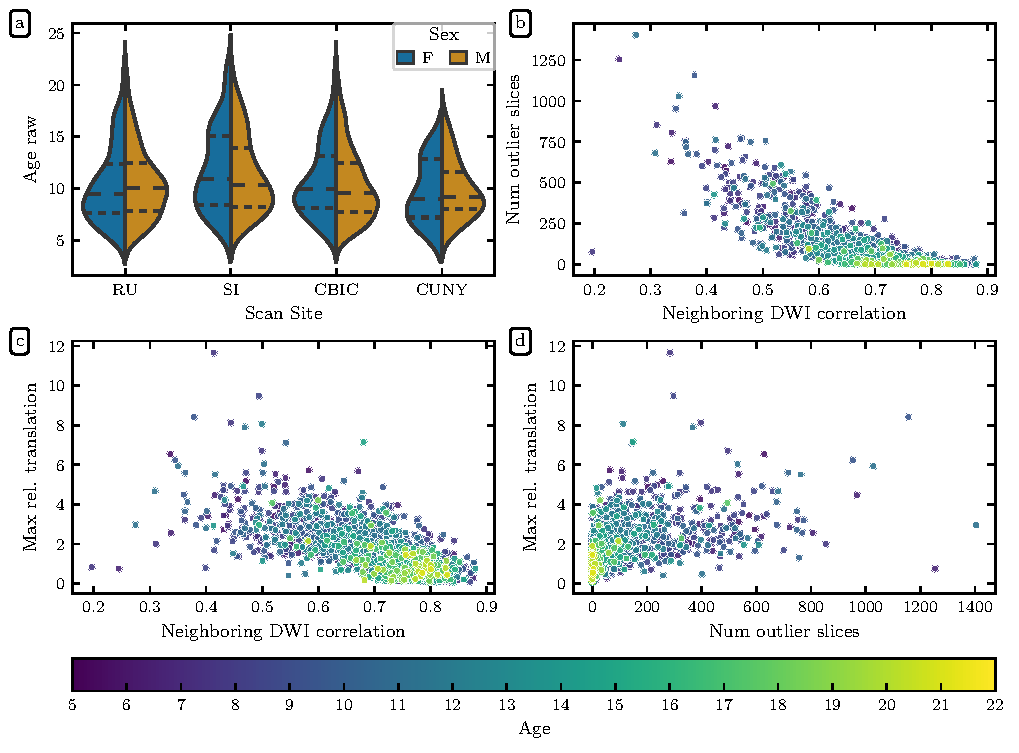
\includegraphics[width=\linewidth]{qsiprep-metric-distributions.pdf}
    \caption{%
        {\bf Demographic and \emph{QSIPrep} quality metric distributions}:
        \textbf{(a)} HBN age distributions by sex for each scanning site. Dashed lines
        indicate age quartiles.
        %
        The remaining plots show associations between \textbf{(b)} neighboring
        diffusion-weighted imaging (DWI) correlation  \cite{yeh2019-kb} and the
        number of outlier slices, \textbf{(c)} neighboring DWI correlation and maximum relative
        translation, and \textbf{(d)} the number of outlier slices and maximum
        relative translation.
        %
        The number of outlier slices is positively associated with the maximum
        relative translation, while neighboring DWI correlation is negatively associated with the other
        two metrics.
        %
        These plots are colored by age, and reveal that older participants
        generally have higher quality data.
    }
    \label{fig:metric-dist}
\end{figure}

\begin{longtable}{p{4.0cm}p{2.9cm}p{9.3cm}}
\caption{HBN-POD2 data records} \label{tab:data-records} \\
\toprule
    Data Resource & Repositories & Location \\
\midrule
\endfirsthead

\toprule
    Data Resource & Repositories & Location \\
\midrule
\endhead
\midrule
\multicolumn{2}{r}{{Continued on next page}} \\
\midrule
\endfoot

\hline
\hline
\multicolumn{3}{l}{{$\dagger$ FCP-INDI: all paths are relative to the root \url{s3://fcp-indi/data/Projects/HBN/BIDS_curated/}}} \\
%
\multicolumn{3}{l}{{$\diamondsuit$ HBN-POD2 DataLad dataset\cite{hbnpod2data}: use \texttt{datalad clone git@github.com:nrdg/HBN-POD2.git}.}} \\
\multicolumn{3}{l}{{\hspace{5em}All paths are relative to the repository root.}} \\
%
\multicolumn{3}{l}{{$\Join$ \emph{QSIPrep} derivatives dataset\cite{hbnpod2qsiprepdata}:}} \\
\multicolumn{3}{l}{{\hspace{5em}use \texttt{datalad clone git@github.com:nrdg/HBN-POD2-derivatives-qsiprep.git}.}} \\
\multicolumn{3}{l}{{\hspace{5em}All paths are relative to the repository root.}} \\
%
\multicolumn{3}{l}{{$\square$ \emph{AFQ} derivatives dataset\cite{hbnpod2afqdata}:}} \\
\multicolumn{3}{l}{{\hspace{5em}use \texttt{datalad clone git@github.com:nrdg/HBN-POD2-derivatives-afq.git}.}} \\
\multicolumn{3}{l}{{\hspace{5em}All paths are relative to the repository root.}} \\
\multicolumn{3}{l}{{* participants.tsv: located on FCP-INDI and in the HBN-POD2 DataLad dataset at relative path}} \\
\multicolumn{3}{l}{{\hspace{5em}\texttt{derivatives/qsiprep/participants.tsv}, and in the HBN-POD2 \emph{QSIPrep} derivatives DataLad}} \\
\multicolumn{3}{l}{{\hspace{5em}dataset at \texttt{participants.tsv}}} \\
\multicolumn{3}{l}{{$\ddagger$ HBN-POD2 OSF Project\cite{hbn-pod2-osf}: all paths are relative to the root \texttt{HBN-POD2 QC/OSF Storage}}} \\
\bottomrule
\endlastfoot
    BIDS Curated Imaging
        & FCP-INDI\textsuperscript{$\dagger$}
        & \texttt{/} \\
        & DataLad dataset\textsuperscript{$\diamondsuit$}
        & \texttt{/} \\
    \hline
    \emph{QSIPrep} preprocessed DWI
        & FCP-INDI\textsuperscript{$\dagger$}
        & \texttt{/derivatives/qsiprep/} \\
        & DataLad dataset\textsuperscript{$\diamondsuit$}
        & \texttt{/derivatives/qsiprep/} \\
        & \emph{QSIPrep} dataset\textsuperscript{$\Join$}
        & \texttt{/} \\
    \hline
    CuBIDS variants
        & \texttt{participants}*
        & \texttt{site\_variant} column  \\
    \hline
    Raw expert ratings
        & OSF\textsuperscript{$\ddagger$}
        & \texttt{/expert-qc/} \\
    \hline
    Expert QC scores
        & \texttt{participants}*
        & \texttt{expert\_qc\_score} column \\
    \hline
    Raw community ratings
        & OSF\textsuperscript{$\ddagger$}
        & \texttt{/community-qc/} \\
    \hline
    Community QC scores
        & \texttt{participants}*
        & \texttt{xgb\_qc\_score} column \\
    \hline
    QSIQC QC scores
        & \texttt{participants}*
        & \texttt{xgb\_qsiprep\_qc\_score} column \\
    \hline
    QSIQC model
        & GitHub
        & DOI: \href{https://doi.org/10.5281/zenodo.5949269}{10.5281/zenodo.5949269} \\
    \hline
    Deep learning input images
        & FCP-INDI\textsuperscript{$\dagger$}
        & \texttt{/derivatives/qsiprep/derivatives/dlqc/} \\
    \hline
    Deep learning models
        & OSF\textsuperscript{$\ddagger$}
        & \texttt{/deep-learning-qc/saved-models} \\
    \hline
    Deep learning QC scores
        & \texttt{participants}*
        & \texttt{dl\_qc\_score} column \\
    \hline
    Deep learning attributions
        & OSF\textsuperscript{$\ddagger$}
        & \texttt{/deep-learning-qc/integrated-gradients} \\
    \hline
    \multirow{2}{4.0cm}{AFQ tractography \& tractometry}
        & FCP-INDI\textsuperscript{$\dagger$}
        & \texttt{/derivatives/afq/} \\
        & DataLad dataset\textsuperscript{$\diamondsuit$}
        & \texttt{/derivatives/afq/} \\
        & \emph{AFQ} dataset\textsuperscript{$\square$}
        & \texttt{/} \\
    \hline
    \added{AFQ streamline counts}
        &
        FCP-INDI\textsuperscript{$\dagger$}
        &
        \texttt{/derivatives/afq/participants.tsv} \\
        & DataLad dataset\textsuperscript{$\diamondsuit$}
        &
        \texttt{/derivatives/afq/participants.tsv} \\
        & \emph{AFQ} dataset\textsuperscript{$\square$}
        & \texttt{/participants.tsv} \\
    \hline
    AFQ tract profiles
        & FCP-INDI\textsuperscript{$\dagger$}
        & \texttt{/derivatives/afq/combined\_tract\_profiles.csv} \\
        & DataLad dataset\textsuperscript{$\diamondsuit$}
        & \texttt{/derivatives/afq/combined\_tract\_profiles.csv} \\
        & \emph{AFQ} dataset\textsuperscript{$\square$}
        & \texttt{/combined\_tract\_profiles.csv} \\
\end{longtable}

\subsection*{CuBIDS Variants
\comment{The contents of this subsection were previously in an appendix. We have moved it to the main text at the editor's request.}
}

We identified 20 unique dMRI acquisitions across HBN-POD2, which are summarized in Table~\ref{tab:variants}. Site CBIC has two acquisition types: ``64dir,'' which shares its pulse sequence with sites RU and CUNY, and ``ABCD64dir,'' with acquisition parameters that better match the ABCD study (TE=\qty{0.089}{\second} and TR=\qty{4.1}{\second}). The ``Most\_Common'' variant identifies the most common combination of acquisition parameters for a given site and acquisition. The ``Low\_Volume'' variant identifies participants from all sites with less that 129 DWI volumes, which is the number of volumes in the most common variants. All remaining variants names identify the acquisition parameter(s) that differ from those of the most common variant. For example, the ``MultibandAccelerationFactor'' variant has a different multiband acceleration factor than that of the the most common variant but all participants within that variant share the same multiband acceleration factor. Variants that differ by multiple acquisition parameters have names that are composed of concatenated parameters. For example, the variant ``Dim3SizeVoxelSizeDim3'' varies both in the number of voxels in dimension 3 (``Dim3Size'') and in the voxel size in dimension 3 (``VoxelSizeDim3'').

The specific variant of each scanning session is provided as a column in the HBN-POD2 participant.tsv file. 
Users may use this information to test their BIDS-Apps on a subset of participants that represent the full range of acquisition parameters that are present.

\begin{table}[htbp]
\centering
\begin{tabular}{lllr}
\toprule
     Site &      Acquisition &                        Variant &  Count \\
\midrule
     CBIC &            64dir &                    Most\_Common &    828 \\
     CBIC &            64dir &                      Obliquity &     32 \\
     CBIC &            64dir &     VoxelSizeDim1VoxelSizeDim2 &      1 \\
     CBIC &        ABCD64dir &                    Most\_Common &     15 \\
     CBIC &        ABCD64dir &                        HasFmap &      2 \\
     CBIC &        ABCD64dir &    MultibandAccelerationFactor &      1 \\
     CBIC &        ABCD64dir &                      Obliquity &      1 \\
     CUNY &            64dir &                    Most\_Common &     68 \\
     CUNY &            64dir &          Dim3SizeVoxelSizeDim3 &      4 \\
     CUNY &            64dir &                      Obliquity &      2 \\
       RU &            64dir &                    Most\_Common &    859 \\
       RU &            64dir &                         NoFmap &      5 \\
       RU &            64dir &                      Obliquity &      8 \\
       RU &            64dir &         PhaseEncodingDirection &      1 \\
       SI &            64dir &                       EchoTime &      1 \\
       SI &            64dir & EchoTimePhaseEncodingDirection &      9 \\
       SI &            64dir &                    Most\_Common &    269 \\
       SI &            64dir &                         NoFmap &      2 \\
       SI &            64dir &                      Obliquity &     12 \\
All Sites & All Acquisitions &               Low\_Volume\_Count &     14 \\
\bottomrule
\end{tabular}
\caption{%
  Participant counts for HBN-POD2 variants.
  \label{tab:variants}
}
\end{table}


\subsection*{Quality control data}
%%%%%%%%%%%%%%%%%%%%%%%%%%%%%%%%%%%%%%%%

We provide four separate QC scores in the \texttt{participants.tsv} file described in Table~\ref{tab:data-records}. The mean expert ratings are available in the ``expert\_qc\_score'' column.
These ratings are scaled to the range \numrange{0}{1}, so that a mean rating from \numrange{0}{0.2} corresponds to an expert rating of ``definitely fail'', a mean rating from \numrange{0.2}{0.4} corresponds to ``probably fail'', from \numrange{0.4}{0.6} corresponds to ``not sure'', from \numrange{0.6}{0.8} corresponds to ``probably pass'', and \numrange{0.8}{1.0} corresponds to ``definitely pass.''
The XGB model's positive class probabilities are available in the ``xgb\_qc\_score'' column,
while the XGB-q model's positive class probabilities are available in the ``xgb\_qsiprep\_qc\_score'' column.
Finally, the CNN-i+q model's positive class probabilities are available in the ``dl\_qc\_score'' column.

\subsection*{Tractography and tractometry}
%%%%%%%%%%%%%%%%%%%%%%%%%%%%%%%%%%%%%%%%

The outputs of the pyAFQ tractometry pipeline, including tractography and tract profiles, are provided as specified in Table~ref{tab:data-records}: in a BIDS derivative directory in the FCP-INDI AWS S3 bucket, as a Datalad dataset\cite{hbnpod2afqdata} and as a DataLad subdataset in the primary HBN-POD2 dataset\cite{hbnpod2data}. In particular the FA and MD tract profiles for each participants are available on S3 at \url{s3://fcp-indi/data/Projects/HBN/BIDS_curated/derivatives/afq/combined_tract_profiles.csv}.
\added[comment=We added information on the streamline counts file in response to Reviewer~\#2]{Streamline counts for each of the bundles are available at \url{s3://fcp-indi/data/Projects/HBN/BIDS_curated/derivatives/afq/participants.tsv}}

For each subject, intermediate data derivatives of the pyAFQ pipeline are also provided. 

\begin{itemize}

\item A brain mask and mean b=0 image are saved with ``\texttt{\_brain\_mask.nii.gz}'' and ``\texttt{\_b0.nii.gz}'' file-name suffixes. A set of diffusion modeling derivatives are saved for each of  three different diffusion models: DTI, DKI and CSD. Diffusion model parameters are saved with the ``\texttt{\_diffmodel.nii.gz}'' suffix. Derived model scalars are saved with suffixes that indicate the model and the scalar. For example, the FA derived from the DTI model is saved with the ``\texttt{\_DTI\_FA.nii.gz}'' suffix. 

\item Masks used to initialize tractography are saved with the ``\texttt{seed\_mask.nii.gz}'' suffix, while those used to determine the stopping criterion for tractography are stored with  the ``\texttt{stop\_mask.nii.gz}'' suffix. 

\item Files that define a non-linear transformation between the individual subject anatomy and the MNI template for the purpose of waypoint ROI placement are stored with ``\texttt{mapping\_from-DWI\_to\_MNI\_xfm.nii.gz}'' (non-linear component) and ``\texttt{prealing\_from-DWI\_to\_MNI\_xfm.npy}'' (affine component) suffixes. The waypoint ROIs, transformed to the subject anatomy through this non-linear transformation are also stored in the ``ROIs'' sub-directory.

\item Tractography derivatives are stored with the ``\texttt{\_tractography.trk}''. The whole-brain tractography, which serves as the input data for bundle segmentation, is stored with the ``\texttt{\_CSD\_desc-prob\_tractography.trk}'' suffix. Streamlines that were selected for inclusion in one of the major bundles are stored in separate files in the ``bundles'' sub-directory and saved in a consolidated file with the ``\texttt{CSD\_desc-prob-afq\_tractography.trk}'' suffix. The streamlines selected for inclusion and also additionally cleaned through a process of outlier removal are stored with the ``\texttt{CSD\_desc-prob-afq-clean\_tractography.trk}'' suffix and also in a ``clean\_bundles'' sub-directory. 

\item An interactive visualization of bundles relative to the individual anatomy is stored with the ``\texttt{\_viz.html}'' suffix and summaries of streamline counts in each bundle are stored with the ``\texttt{\_sl\_count.csv}''. Additional visualizations are provided in the ``tract\_profile\_plots'' and ``viz\_bundles'' sub-directory.

\item Individual tract profiles are stored with the ``\texttt{afq\_profiles.csv}'' suffix. This information is redundant with the one provided in aggregate format in the ``\texttt{combined\_tract\_profiles.csv}'' file.

\item \added[comment=We added an item for the bundle streamline counts output]{Individual streamline counts for each of the bundles are stored with the ``\texttt{\_sl\_count.csv}'' suffix. This information is redundant with the one provided in aggregate format in the ``\texttt{participants.tsv}'' file.}

\end{itemize}

%%%%%%%%%%%%%%%%%%%%%%%%%%%%%%%%%%%%%%%%%%%%%%%%%%%%%%%%%%%%
\section*{Technical Validation}
%%%%%%%%%%%%%%%%%%%%%%%%%%%%%%%%%%%%%%%%%%%%%%%%%%%%%%%%%%%%

\subsubsection*{Attribution masks for the deep learning classifier}

We generated post-hoc attribution maps that highlight regions of the input
volume that are relevant for the deep learning generated QC scores. The integrated gradient method
\cite{sundararajan2017axiomatic} is a gradient-based attribution method
\cite{ancona2019gradient} that aggregates gradients for synthetic images
interpolating between a baseline image and the input image. It has been used to
interpret deep learning models applied to retinal imaging in diabetic
retinopathy \cite{sayres2019using} and glaucoma \cite{Mehta2021-zp} prediction,
as well as in multiple sclerosis prediction from brain MRI
\cite{wargnier-dauchelle2021interpretable}. Our goal is to confirm that the
CNN-i model
was driven by the same features that would drive the expert rating,
thereby bolstering the decision to apply it to new data.

To generate the attribution maps, we followed Tensorflow's integrated gradients
tutorial \cite{integrated-gradients-tutorial} with a black baseline image and
128 steps in the Riemann sum approximation of the integral (i.e.
\texttt{m\_steps = 128}).

Figure~\ref{fig:ig} shows attribution maps for example participants from each
confusion class: true positive, true negative, false positive, and false
negative. The columns correspond to the different channels of the deep learning
input volume: the $b=0$ reference image and the DEC-FA in the $x$, $y$, and $z$
directions. \added[comment={We added a sentence describing the meaning of the integrated gradient attribution maps in response to Reviewer~\#3 (point~2).}]{These integrated gradients are dimensionless quantities but their sign is meaningful. They are proportional to the probability of assigning one label (``pass'') or another (``fail'')}. 
The blue voxels indicate positive attribution, that is, data that supports a passing QC classification. Conversely, the red voxels indicate negative attribution, data that supports a failing QC classification.
The true positive map indicates that the network was looking at the
entire brain rather than focusing on any one anatomical region
(Figure~\ref{fig:ig:true-pos}). Moreover, the model identified white matter
fascicles that travel along the direction of the input channel: lateral for $x$,
anterior-posterior for $y$, and superior-inferior for $z$. The true negative
attribution map (Figure~\ref{fig:ig:true-neg}) reveals that when the reference
$b=0$ volume contains motion artifacts, such as banding, the network ignored the
otherwise positive attributions for the clearly identifiable white matter tracts
in the DEC-FA channels. The false positive map (Figure~\ref{fig:ig:false-pos})
and the false negative map (Figure~\ref{fig:ig:false-neg}) should be interpreted
differently since they come from low confidence predictions; the probability of
passing hovered on either side of the pass/fail threshold. For example, in the
false positive case, the network was confused enough that it treated voxels that
are outside of the brain to be as informative as voxels in the major white matter bundles.

\begin{figure}[tbp]
    {\phantomsubcaption\label{fig:ig:true-pos}}
    {\phantomsubcaption\label{fig:ig:true-neg}}
    {\phantomsubcaption\label{fig:ig:false-pos}}
    {\phantomsubcaption\label{fig:ig:false-neg}}
    \centering
    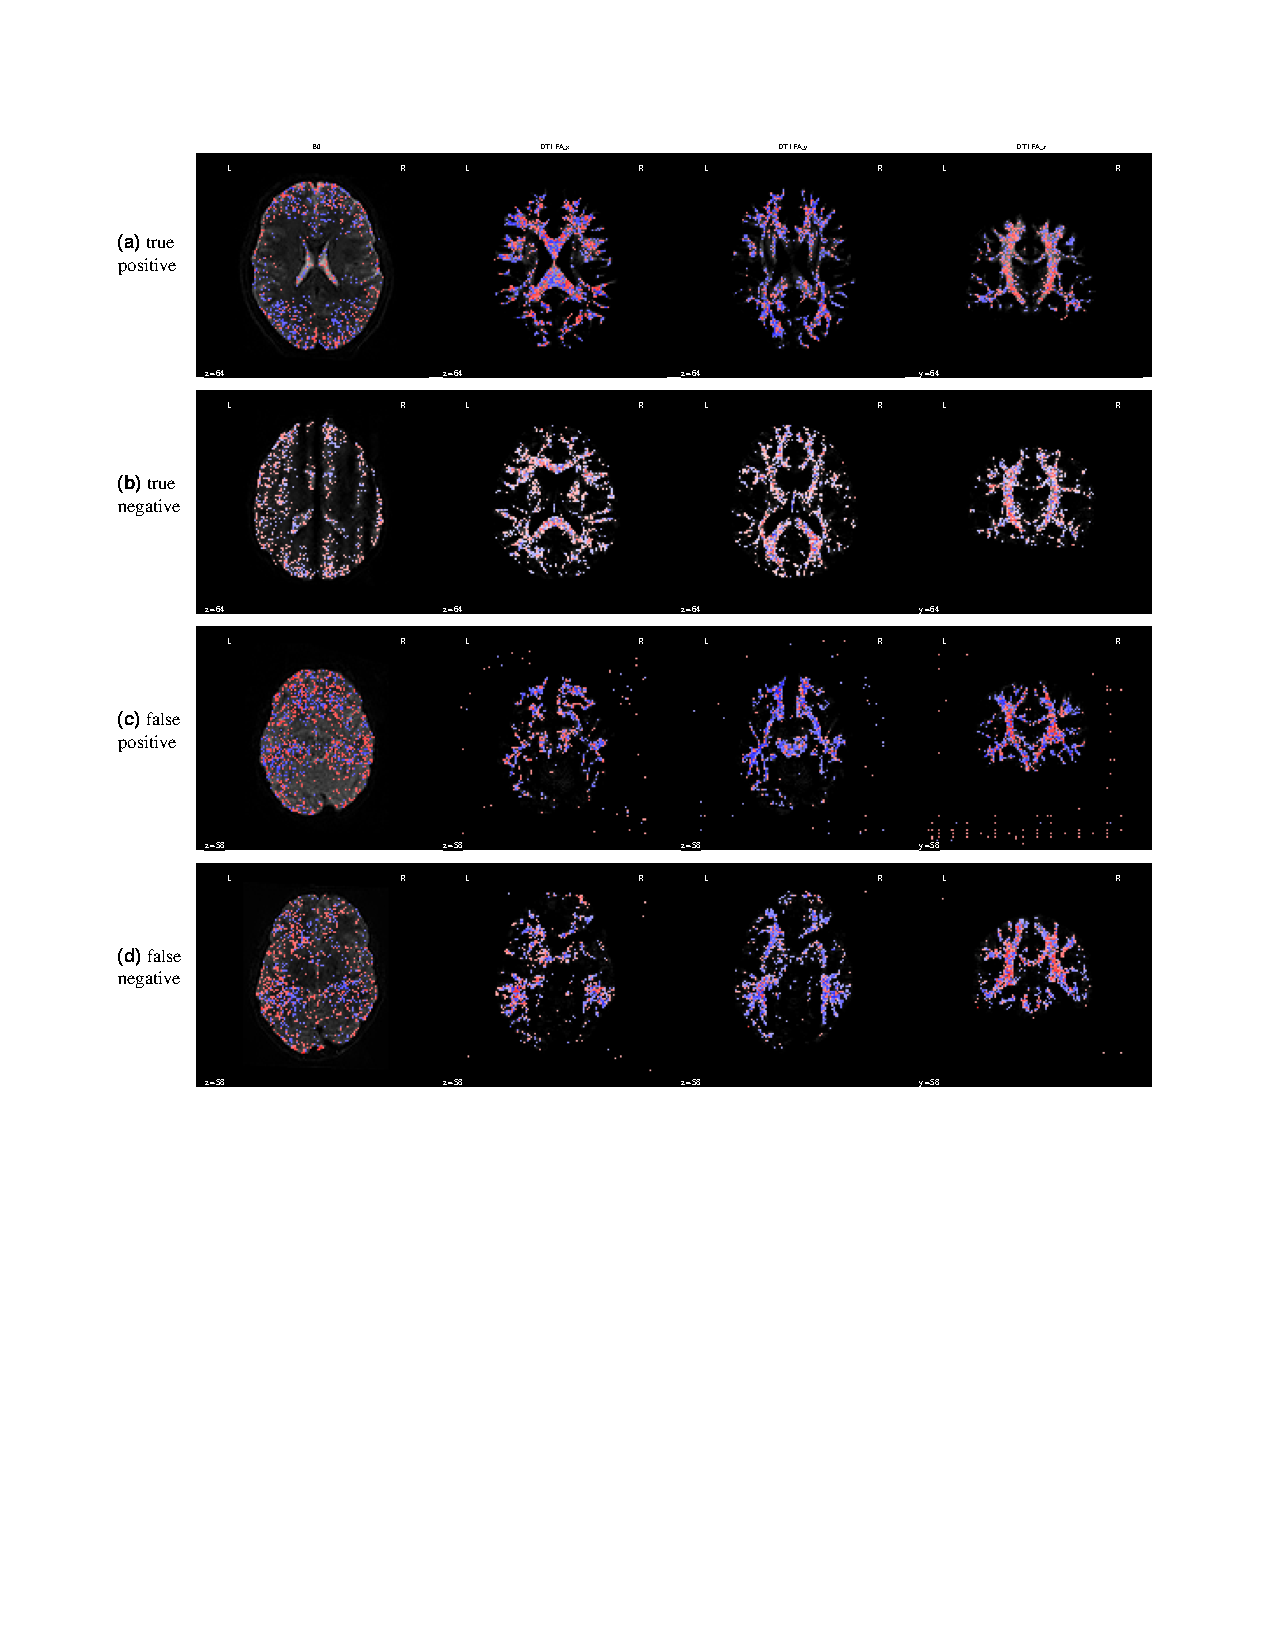
\includegraphics[width=\linewidth]{attribution_maps.pdf}
    \caption{%
        {\bf Integrated gradients attribution maps for the deep learning classifier}:
        Each column depicts a different channel of the input tensor: the $b=0$
        DWI volume and the DEC-FA images in the $x$, $y$, and $z$ directions.
        The first three columns show an axial slice while the last column
        shows a coronal slice. Blue voxels indicate positive attribution (i.e.
        evidence for passing the participant), while red voxels indicate negative
        attribution (i.e. evidence for QC failure). \added{The voxels with small magnitude attribution values ($\leq 98\%$ of the highest value in each image) have been rendered to be transparent, as they do not indicate strong evidence in either direction. In these cases, t}he underlying grayscale
        depicts the input channel \added{($b=0$ or $x$, $y$, or $z$ elements of the DEC-FA image)}. Each row depicts a representative participant
        from each confusion class:
        %
        \textbf{(a)} Attribution maps for a true positive prediction. The model
        looked at the entire brain and focused on known white matter bundles in
        the DEC-FA channels. In particular, it focused on lateral bundles in the
        $x$ direction, anterior-posterior bundles in the $y$ direction, and
        superior-inferior bundles in the $z$ direction.
        %
        \textbf{(b)} Attribution maps for a true negative prediction. The model
        focused primarily on the $b=0$ channel, suggesting that it ignores
        DEC-FA when motion artifacts like banding are present.
        %
        \textbf{(c)} Attribution maps for a false positive prediction. Both the
        false positive and negative predictions were low confidence predictions.
        This is reinforced by the fact that the model viewed some voxels that are outside of the brain as just as informative as those in major white
        matter tracts.
        %
        \textbf{(d)} Attribution maps for a false negative prediction. The model
        failed to find long-range white matter tracts in the anterior-posterior
        and lateral directions. We also speculate that the model expected
        left-right symmetry in the DEC-FA channels and assigned negative
        attribution to asymmetrical features. }
    \label{fig:ig}
\end{figure}

\subsubsection*{QC prediction models can generalize to unseen sites}

Site harmonization is a major issue for any multisite neuroimaging study and developing automated QC tools that generalize between sites has been a perennial issue \cite{esteban2017mriqc}. Furthermore, the ability to generalize between sites in a single multisite study would signal the promise of generalizing to other datasets altogether. To better understand the ability of our QC models to generalize across scanning sites, we trained multiple versions of XGB-q and CNN-i on partitions of the data with different scanning sites held out and then evaluated those models on the held out sites (Figure~\ref{fig:site-generalization} and Table~\ref{tab:site-generalization}). These models were therefore evaluated on data from ``unseen'' sites. We constructed these train/evaluate splits from combinations of the HBN sites with \qty{3}{\tesla} scanners (RU, CBIC, and CUNY), and excluded CUNY as a standalone training or test site because of its low number of participants ($N=74$). This left four combinations of site-generated training splits: CBIC~+~CUNY (eval: RU), CBIC (eval: RU~+~CUNY), RU~+~CUNY (eval: CBIC), and RU (eval: CBIC~+~CUNY).

We trained eight models (with distinct random seeds) from the CNN-i family of models using the global XGB scores as targets, just as with the full CNN-i model. Similarly, we trained twenty models (with distinct random seeds) from the XGB-q family of models using the expert scores as targets, just as with the full XGB-q model. For each model, we reported three evaluation metrics: ROC-AUC, accuracy, and balanced accuracy. Because the distribution of QC scores was imbalanced (Figures~\ref{fig:expert-qc:scatter:hist} and \ref{fig:dl-qc:hist:site}), we included balanced accuracy as an evaluation metric. Balanced accuracy avoids inflated accuracy estimates on imbalanced data \cite{velez2007balanced}, and in the binary classification case, it is the mean of the sensitivity and specificity. For the CNN-i family, we further decomposed the evaluation split into a report set, for which expert scores were available, and a test set, with participants who were not in the ``gold standard'' dataset. For the report set, we evaluated the model using the expert scores as the ground truth. For the test set, we evaluated each model using the XGB scores as ground truth.
Aside from the specification of train and evaluation splits, model training followed exactly the same procedure as for the full dataset. For example, we use the same cross validation and hyperparameter optimization procedure for the XGB-q family as for the original XGB-q model and the same architecture, input format, and early stopping criteria for the CNN-i family as for the CNN-i model.

ROC-AUC for generalization is uniformly high for both the XGB-q and the CNN-i models. However, more importantly, accuracy and balanced accuracy vary substantially: depending on the site that was used for training, balanced accuracy could be as low as guess rate, particularly for the CNN-i model. Notably, it seems that including the RU site in the training data led to relatively high balanced accuracy in both models. The XGB-q model balanced accuracy was less dependent on the specific sites used for training, but also displayed some variability across permutations of this experiment. In particular, the benefit from including the ``right site'' in the training data, namely RU, eclipsed the slight benefit conferred by including more than one site in the training data.

\begin{figure}[tbp]
    {\phantomsubcaption\label{fig:site-generalization:dl}}
    {\phantomsubcaption\label{fig:site-generalization:xgb}}
    \centering
    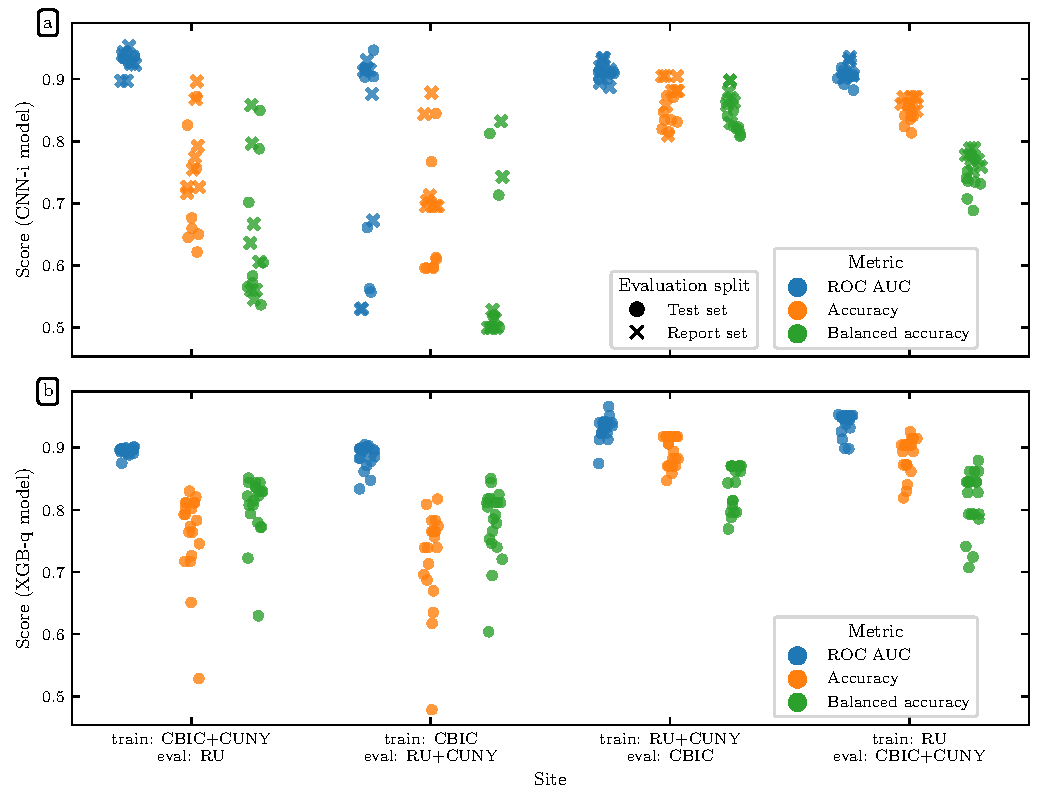
\includegraphics[width=\linewidth]{site_generalization.pdf}
    \caption{%
        {\bf Generalization of QC scores to unseen sites}: In each experiment, CNN-i (\textbf{a}) and XGB-q (\textbf{b}) models were trained with some sites held out and evaluated only on data from these held out sites. Model performance is quantified as ROC-AUC (blue), accuracy (orange) and balanced accuracy (green). For XGB-q, the targets are the expert ratings on data from the held out site. For CNN-i, performance is scored against XGB scores (as used before; test set in filled circles), or expert ratings on the data from the held out site (report set in crosses). Summary statistics for this plot are listed in Table~\ref{tab:site-generalization}.
    }
    \label{fig:site-generalization}
    \vspace{1em}
    \captionof{table}{%
        {\bf Site generalization summary statistics}:
        Below we list the mean $\pm$ standard deviation of the site generalization evaluation metrics displayed in Figure~\ref{fig:site-generalization}.
        For each of the CNN-i and XGB-q model families and each of the site generalization splits, we report the accuracy, balanced accuracy, and ROC-AUC.
    }
    \begin{tabular}{lllll}
    \toprule
          &                            &       Accuracy & Balanced accuracy &        ROC-AUC \\
    Model & Site &                &                   &                \\
    \midrule
    CNN-i & train: CBIC + CUNY, test: RU &  $0.748 \pm 0.086$ &     $0.652 \pm 0.112$ &  $0.930 \pm 0.015$ \\
          & train: CBIC, test: RU + CUNY &  $0.696 \pm 0.095$ &     $0.574 \pm 0.123$ &  $0.791 \pm 0.169$ \\
          & train: RU + CUNY, test: CBIC &  $0.859 \pm 0.033$ &     $0.847 \pm 0.030$ &  $0.912 \pm 0.013$ \\
          & train: RU, test: CBIC + CUNY &  $0.851 \pm 0.018$ &     $0.753 \pm 0.029$ &  $0.910 \pm 0.014$ \\
    XGB-q & train: CBIC+CUNY, test: RU   &  $0.763 \pm 0.071$ &     $0.805 \pm 0.052$ &  $0.895 \pm 0.006$ \\
          & train: CBIC, test: RU+CUNY   &  $0.725 \pm 0.079$ &     $0.779 \pm 0.058$ &  $0.886 \pm 0.019$ \\
          & train: RU+CUNY, test: CBIC   &  $0.894 \pm 0.024$ &     $0.838 \pm 0.036$ &  $0.931 \pm 0.018$ \\
          & train: RU, test: CBIC+CUNY   &  $0.886 \pm 0.030$ &     $0.816 \pm 0.048$ &  $0.940 \pm 0.017$ \\
    \bottomrule
    \end{tabular}
    \label{tab:site-generalization}
\end{figure}

\subsection*{Quality control improves inference}
%%%%%%%%%%%%%%%%%%%%%%%%%%%%%%%%%%%%%%%%

To demonstrate the effect that quality control has on inference, we analyzed tract profile data derived from HBN-POD2 data. 

Missing values were imputed using median imputation as implemented by \emph{scikit-learn}'s \texttt{SimpleImputer} class. Because the HBN-POD2 bundle profiles exhibit strong site effects \cite{richie-halford2021multidimensional}, we used the ComBat harmonization method to robustly adjust for site effects in the tract profiles \cite{Johnson2007-kl, fortin2018-hk, fortin2017-be, nielson2018detecting}, using the \emph{neurocombat\_sklearn} library \cite{neurocombat-sklearn}.

In Figure~\ref{fig:age-prediction}, we plot the mean diffusivity (MD) and fractional anisotropy (FA) profiles along the left superior longitudinal fasciculus (SLFL) grouped into four QC bins.
The SLFL exhibits strong differences between
QC bins. Low QC scores tend to flatten the MD and FA profiles, indicating that MD and FA appear artifactually homogeneous across the bundle.

The effect of QC score on white matter bundle profiles indicates that researchers
using HBN-POD2 should incorporate QC in their analyses, either by applying a QC cutoff
when selecting participants or by explicitly adding QC score to their inferential
models. Failure to do so may cause spurious associations or degrade predictive
performance. To demonstrate this, we selected participant age as a representative phenotypic benchmark because
\begin{enumerate*}[%
    label=(\roman*),%
    before=\unskip{ },%
    itemjoin={{, }},%
    itemjoin*={{ and }}]
    \item it operates on a natural scale with meaningful units
    \item despite the unique methodological challenges it presents for biomarker identification \cite{nelson2020biomarkers}, brain age prediction may be diagnostic of overall brain health \cite{franke2010estimating, cole2019brain, richie-halford2021multidimensional}.
\end{enumerate*}
We observed the effect of varying QC cutoff on the predictive performance of an age
prediction model (Figure~\ref{fig:age-prediction}).

\begin{figure}[tbp]
    \centering
    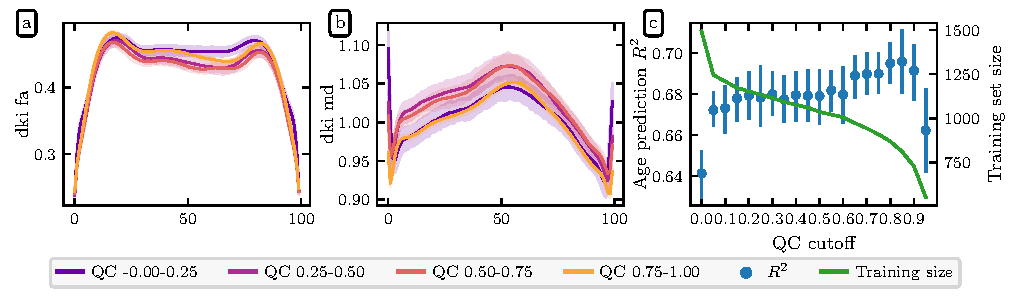
\includegraphics[width=\linewidth]{qc_sweep.pdf}
    \caption{%
        {\bf Imposing a QC cutoff improves age prediction}:
        Cross validated $R^2$ scores (left axis, blue dots) from an age
        prediction model increase after screening participants by QC score. We see
        the most dramatic increase in $R^2$ after imposing even the lowest
        cutoff of $0.05$. Thereafter, the $R^2$ scores trend upward until a
        cutoff of $\sim 0.95$, where the training set size (right axis, orange
        line) becomes too small to sustain model performance. The error bands
        represent a bootstrapped 95\% confidence interval.
    }
    \label{fig:age-prediction}
\end{figure}

We evaluated this effect by observing cross-validated $R^2$ values of gradient boosted trees models implemented using XGBoost. The input feature space for each model consisted of \num{4800} features per participant, comprising 100 nodes for each of MD and FA in the twenty-four major tracts. We imputed missing bundles and harmonized the different scanning sites as above. The XGBoost models' hyperparameters were hand-tuned to values that have been performant in the authors' previous experience.
Within the limited age range of the HBN study, MD and FA follow logarithmic maturation trajectories \cite{yeatman2014lifespan}. We therefore log-transformed each participant's age before prediction using the \texttt{TransformedTargetRegressor} class from \emph{scikit-learn}.
For each value of the QC cutoff between 0 and 0.95, in steps of 0.05, we computed the cross-validated $R^2$ values using \emph{scikit-learn}'s \texttt{cross\_val\_score} function with repeated K-fold cross-validation using five folds and five repeats.

Cross-validated $R^2$ scores for an age prediction model varied depending on the QC cutoff (Figure~\ref{fig:age-prediction}). An initial large improvement was achieved by excluding the 200 participants with the lowest QC scores, followed by a gradual increase in performance. Finally, when a large number of participants is excluded, performance deteriorated again.

%%%%%%%%%%%%%%%%%%%%%%%%%%%%%%%%%%%%%%%%%%%%%%%%%%%%%%%%%%%%
\section*{Usage Notes}
%%%%%%%%%%%%%%%%%%%%%%%%%%%%%%%%%%%%%%%%%%%%%%%%%%%%%%%%%%%%

HBN-POD2 is one of the largest child and adolescent diffusion imaging
datasets with preprocessed derivatives that is currently openly available. The dataset
was designed to comply with the best practices of the field. For example, it
complies with the current draft of the BIDS diffusion derivative specification
\cite{Pestilli2021}. It will grow continuously as the HBN study acquires more
data, eventually reaching its \num{5000} participant goal. 

\subsection*{Preprocessing and quality control increase the impact of openly-available data}
%%%%%%%%%%%%%%%%%%%%%%%%%%%%%%%%%%%%%%%%

The HBN-POD2 data is amenable to many different analyses, including
tractometry \cite{yeatman2012-rc, yeatman2018browser, kruper2021evaluating}, graph theoretical analysis \cite{yeh2020-nu},
and combinations with functional MRI data and other data types for the same
participants. The availability of standardized preprocessed diffusion data will
allow researchers to create and test hypotheses on the white matter properties
underlying behavior and disease, from reading and math acquisition to childhood
adversity and mental health. As such, this dataset will accelerate discovery at
the nexus of white matter microstructure and neurodevelopmental and learning
disorders.

In large developmental datasets, it is critically important to perform accurate and reliable QC of
the data.
QC is associated not just with age, but with many
phenotypic variables of interest in cognition and psychopathology \cite{siegel2017quality}.
HBN-POD2 provides four separate QC scores alongside its large dataset
of pediatric neuroimaging diffusion derivatives, paving the way for users of the
data to incorporate considerations of data quality into their analysis of the
processed data. Unsurprisingly, QC scores are strongly correlated with
age (Figure~\ref{fig:dl-qc}). This accords with the negative association
between head motion and age in developmental studies, which is well established both in general
\cite{power2012spurious,satterthwaite2012impact,fair2012distinct,yendiki2014spurious}
and specifically for resting-state fMRI in the HBN dataset \replaced[comment=We added the source dataset citation at the editor's request.]{\cite{alexander2017yc, hbndata}}{\cite{alexander2017yc}}.
Moreover, it is important that QC has bundle-specific and spatially localized effects (Figure~\ref{fig:qc-profiles:md}). Analysis of this data that does not incorporate QC is likely to find replicable but invalid effects. For example, in patient-control studies, patients are likely to have lower quality data. And analysis of such patient data that does not control for QC will find spatially-localized and replicable group differences that are due to data quality, not necessarily underlying neuroanatomical differences.

We further demonstrated the impact of QC in a benchmark age prediction task
(Figure~\ref{fig:age-prediction}). In this case, the increase in model performance
from imposing a QC cutoff is intuitive: we know from
Figure~\ref{fig:qc-profiles:md} that participants with low QC scores have
reduced MD, but MD also decreases as participants mature
\cite{yeatman2014lifespan,richie-halford2021multidimensional}. Eliminating
participants with low QC therefore removes the ones who may look artificially older
from the analysis, improving overall performance. The most noticeable
improvement in performance comes after imposing the most modest cutoff of
$0.05$, suggesting that inferences may benefit from \emph{any} QC screening. On
the other hand, QC screening inherently introduces a tradeoff between the desire
for high quality data and the desire for a large sample size. In this case,
after a QC cutoff of around $0.9$, the training set size is reduced such that it
degrades predictive performance. Importantly, we do not expect the sensitivity
analysis of an age prediction model to generalize to other analyses and therefore
recommend that researchers using HBN-POD2 choose the most appropriate QC cutoff for their research question and consider including QC score as a model covariate in their analyses.

\subsection*{Automated quality control: scalability, interpretability, and generalization}
%%%%%%%%%%%%%%%%%%%%%%%%%%%%%%%%%%%%%%%%

The predictive
performance of the CNN-i model (Figure~\ref{fig:dl-qc:roc}) gives
us confidence that it could accurately classify unseen data from the same sites, justifying its
extension to the entire HBN-POD2 dataset and to future releases of HBN. However, one limitation of this model is that it
does not satisfactorily explain its decisions. As deep learning models have been increasingly
applied to medical image analysis, there is an evolving interest in the
interpretability of these models \cite{salahuddin2022transparency, lipton2017doctor,
Zech2018-ki, Ghassemi2021-zg}. While an
exhaustive interpretation of deep learning QC models is beyond the scope of this
work, we provided a preliminary qualitative interpretation of the CNN-i model
(Figure~\ref{fig:ig}) that demonstrates the intuitive nature of its decisions. 

The accuracy in generalizing to unseen data from HBN also suggested the tantalizing possibility that the QC models would be able to generalize to similar data from other datasets. To assess this, we trained the models with unseen sites held out (Figure \ref{fig:site-generalization}). Both the CNN-i model and the XGB-q model do sometimes generalize to data from unseen sites, suggesting that they would be able to generalize to some other datasets as well. However, they do not reliably generalize, implying that they should not currently be used in this way. Future work could build upon the work that we have done here to establish a procedure whereby the models that we fit in HBN would be applied to data from other studies, but comprehensive calibration and validation would have to be undertaken as part of this procedure. 

We recognize that decisions about QC \replaced{exclusion}{inclusion} must balance accuracy, interpretability, generalization to new data, and scalability to ever larger datasets. We therefore provide three additional scores
\begin{enumerate*}[%
    label=(\roman*),%
    before=\unskip{: },%
    itemjoin={{, }},%
    itemjoin*={{, and }}]
    \item the mean expert QC score for the 200 participants in the gold standard
    dataset
    \item the scores predicted by the XGB model, which outperformed all other models
    when evaluated against the gold standard ratings, but which are only available
    for participants that have community science scores
    \item the scores predicted by the XGB-q model, which underperformed the deep
    learning generated scores, but which rely only on the automated QC metrics
    output by \emph{QSIPrep}.
\end{enumerate*}
We view the XGB-q scores, which are available for all participants, as a more interpretable and scalable fallback because the XGB-q model ingests \emph{QSIPrep} output without any further postprocessing. XGB-q also provides slightly more uniform performance in generalization to unseen HBN sites (Figure~\ref{fig:site-generalization}). Because the XGB-q model most readily generalizes to other \emph{QSIPrep} outputs, we package it as an independent QC service in the QSIQC software package \cite{richiehalford2022qsiqc}, available both as a docker image at \texttt{ghcr.io/richford/qsiqc} and as a Streamlit app at \url{https://share.streamlit.io/richford/qsiqc/main/app.py}.
The decision to use a more interpretable but slightly less
performant method of generating QC scores was also advocated by
\cite{tobe2021longitudinal}, who noted that the Euler number of T1-weighed
images \cite{rosen2018quantitative} in the NKI-Rockland dataset can reliably predict scores generated with
\emph{Braindr}, the community science application developed in our previous work
\cite{keshavan2019-er}.

We also note that the issue of algorithmic impact in choosing a QC method is not
exclusive to the deep learning model. We have chosen models that most reliably
reproduce the gold standard ratings, but a reliable algorithm might still
negatively influence researcher's decisions. For example, excluding participants
by QC score could spur them to exclude populations deserving of study, as when
QC score is highly correlated with age or socio-economic status. We therefore
caution researchers to examine interactions between the QC scores we provide and
their phenotype of interest.

More generally, QC in the dataset that we have produced is fundamentally
anchored to the decisions made by the expert observers. While Cohen's $\kappa$
between some pairs of experts can be as low as 0.52, IRR quantified across all
of the experts with ICC3k is excellent. Nevertheless, it is possible that
improvements to the final QC scores could be obtained through improvements to
IRR, or by designing a more extensive expert QC protocol. The tradeoff between
more extensive QC for each participant and more superficial QC on more participants was
not explored in this study, but could also be the target for future research.

\added[comment={In response to Reviewer~2 (point~5), we added a paragraph recommending the use of other metrics for inclusion criteria.}]{Finally, the QC scores in this dataset are single scalar representations of the quality of each participant's diffusion weighted imaging. They should not be taken as a single measurement of suitability for inclusion. QC metrics are exclusion metrics, not inclusion metrics. In fact, we postulate that no single measurement is suitable as an inclusion criterion \emph{by itself}. For example, some HBN participants have both neuroanatomical abnormalities and high quality diffusion data, as measured by high neighboring DWI correlation, low framewise displacement, and high QC scores. Therefore, one would need to include other sources of information when considering inclusion in a particular study. For example, we recommend that users consult the pyAFQ streamline counts (see Table~\ref{tab:data-records}) to assess suitability for inclusion in a study of normative brains.}

\subsection*{Transparent pipelines provide an extensible baseline for future methods}
%%%%%%%%%%%%%%%%%%%%%%%%%%%%%%%%%%%%%%%%

While the primary audience of HBN-POD2 is researchers in neurodevelopment who
will use the dMRI derivatives in their studies, other researchers may use
HBN-POD2 to develop new preprocessing algorithms or quality control methods. In
this respect, HBN-POD2 follows \cite{avesani2019-ey}, who
recognized the diverse interests that different scientific communities have in
reusing neuroimaging data and coined the term \emph{data upcycling} to promote
multiple-use data sharing for purposes secondary to those of the original
project. Complementing the approach taken in Avesani et al.'s work, which
provided dMRI from a small number of participants preprocessed with many pipelines,
HBN-POD2 contains many participants, all processed with a single state of the art
pipeline, \emph{QSIPrep}. For researchers developing new preprocessing
algorithms, HBN-POD2 provides a large, openly available baseline to which they
can compare their results.

Similarly, neuroimaging QC methods developers will benefit from a large
benchmark dataset of expert, community science, and automated QC ratings, with
which to test new methods. Importantly, the architecture and parameters of the
deep learning network used for QC are also provided as part of this work,
allowing application of this network to future releases of HBN data, and
allowing other researchers to build upon our efforts. Indeed, in this work, we
have extended our previous work on what we now call ``hybrid QC''. This
approach, which we originally applied to the first two releases of the HBN
T1-weighted data \cite{keshavan2019-er} (using the \emph{Braindr} web app:
\url{https://braindr.us}) was extended here in several respects.
First, the \emph{Braindr} study used a smaller dataset of approximately 700
participants, while we extended this approach to well over \num{2000} participants.
Second, \emph{Braindr} relied on approximately \num{80000} ratings from
\num{261} users. Here, we received more than \num{500000} ratings from
\num{374} community scientists. As our understanding of the role of
community scientist contributions has evolved, we decided that we would
include as collective co-authors community scientists who contributed more
than \num{3000} ratings \cite{Ward-Fear2020-zq}.
Third, \emph{Braindr} used data from only a single site. Here, multi-site
data was used. This opens up multiple possibilities for deeper exploration of
between-site quality differences, and also for harmonization of QC across
sites, as we have attempted here.
Last, the most challenging extension of hybrid QC from \emph{Braindr} to
this study entailed developing an approach that would encompass multi-volume
dMRI data. On the one hand, this meant that the task performed by the expert
observers was more challenging, because it required examination of the full
dMRI time-series for every scan. To wit, expert inter-rater reliability was
considerably higher for the T1-weighted only data in \cite{keshavan2019-er}
than for the dMRI data used (Figure~\ref{fig:expert-qc:irr}).
On the other hand, it also meant that the 4D data had to be summarized into
2D data to be displayed in the \emph{Fibr} web application. This was
achieved by summarizing the entire time-series as a DEC-FA + $b=0$ image and
presenting community scientists with animated sections of these images that
showed how the data extended over several horizontal slices.
In addition, the extension to 4D data required developing new deep learning
architectures for analysis of 4D images, including upstream contributions to
\emph{Nobrainer}, a community-developed software library for deep learning
in neuroimaging data \cite{nobrainer}.
These extensions demonstrate that the hybrid QC approach generalizes very well
to a variety of different circumstances. Future applications of this approach
could generalize to functional MRI data, as well as other large datasets from
other kinds of measurements and other research domains.

\subsection*{Future work and open problems}
%%%%%%%%%%%%%%%%%%%%%%%%%%%%%%%%%%%%%%%%

\replaced[comment=We specified the input HBN releases as requested by Reviewer~\#2]{While our work was based on HBN releases 1-9, the}{The} HBN study plans to acquire imaging data for over \num{5000} participants,
necessitating future data releases. \added[comment={This was added in response to Reviewer~\#2's point~2.}]{In particular, the 10th release of HBN data was already made available between completion of the work and the publication of this paper}. Since \added[comment={Added in response to Reviewer~\#2's point~2.}]{this 10th release as well as} future releases of HBN will also require future releases of HBN-POD2, a plan for these is essential. This is
a general issue affecting multi-year neuroimaging projects for which derivative
data is being released before study completion. The use of \emph{QSIPrep},
\emph{cloudknot} and the containerization of the QC score assignment process
facilitate running the exact pipeline described in this paper on newly released
participants. However, this approach is somewhat unsatisfactory because it fails to
anticipate improvements in preprocessing methodology. That is, what should we do
when \emph{QSIPrep} is inevitably updated between HBN releases? Enforce
standardization by using an outdated pipeline or use state-of-the-art
preprocessing at the expense of standardized processing between releases?
Because the use of \emph{cloudknot} and AWS Spot Instances renders preprocessing
fast and relatively inexpensive, we propose a third way: if improvements to the
preprocessing pipeline are available with a new HBN release, we plan to execute
the improved pipeline on the entire HBN dataset, while preserving the previous
baseline release in an archived BIDS derivative dataset.

Undertaking the processing and QC effort to generate HBN-POD2 required
construction and deployment of substantial informatics infrastructure, including
tools for cloud computing, web applications for expert annotation and for
community science rating and analysis software. All of these tools are provided
openly, so that this approach can be generalized even more widely in other
projects and in other scientific fields.

%%%%%%%%%%%%%%%%%%%%%%%%%%%%%%%%%%%%%%%%%%%%%%%%%%%%%%%%%%%%
\section*{Code Availability}
%%%%%%%%%%%%%%%%%%%%%%%%%%%%%%%%%%%%%%%%%%%%%%%%%%%%%%%%%%%%

To facilitate replicability, Jupyter notebooks \cite{kluyver2016jupyter} and
Dockerfiles \cite{merkel2014docker} necessary to reproduce the methods described
herein are provided in the HBN-POD2 GitHub repository at
\url{https://github.com/richford/hbn-pod2-qc}. The specific version of the
repository used in this study is documented in \cite{richiehalford2022hbnpod2qc}.
Most of the code in this repository uses Pandas \cite{mckinney-proc-scipy-2010,reback2020pandas}, Numpy \cite{harris2020array}, Matplotlib \cite{hunter2007matplotlib}, and Seaborn \cite{waskom2021seaborn}.
The \texttt{make} or \texttt{make help} commands will list the available commands and \texttt{make build} will build the requisite Docker images to analyze HBN-POD2 QC data.

In order to separate data from analysis code \cite{Wilson2017-rj}, we provide intermediate data necessary to analyze the QC results in an OSF \cite{Foster-MSLS2017-rl} project \cite{hbn-pod2-osf}, the contents of which can be downloaded using the \texttt{make data} command in the root of the HBN-POD2 GitHub repository. The NIFTI-1 files and TFRecord files provided as input to the CNN models may be separately downloaded using the \texttt{make niftis} and \texttt{make tfrecs} commands, respectively. The remaining \texttt{make} commands and Jupyter notebooks follow the major steps of the methods section:

\begin{enumerate}
    \item The \emph{cloudknot} preprocessing function used to execute \emph{QSIPrep} workflows on curated data was a thin wrapper around \emph{QSIPrep}'s command line interface and is provided
    \replaced[comment={Edited to prevent line breaking across a filename}]{
    in the ``notebooks'' directory of the HBN-POD2 GitHub repository
    in a Jupyter notebook with the suffix \texttt{preprocess-remaining-hbn-curated.ipynb}.
    }{
    in a Jupyter notebook with the suffix \texttt{preprocess-remaining-hbn-curated.ipynb} in the HBN-POD2 GitHub repository in the ``notebooks'' directory.
    }

    \item The expert rating analysis can be replicated using the \texttt{make expert-qc} command in the HBN-POD2 GitHub repository.
    
    \item The \emph{Fibr} community science web application is based on the SwipesForScience framework (\url{swipesforscience.org}), which generates a web application for community science given an open repository of images to be labelled and a configuration file. The source code for the \emph{Fibr} web application is available at \url{https://github.com/richford/fibr}.
    
    \item The images that the \emph{Fibr} raters saw were generated using a \emph{DIPY} \cite{dipy} \texttt{TensorModel} in a \emph{cloudknot}-enabled Jupyter notebook that is available in the ``notebooks'' directory of the \emph{Fibr} GitHub repository. \emph{Fibr} saves each community rating to its Google Firebase backend, the contents of which have been archived to the HBN-POD2 OSF project as specified in Table~\ref{tab:data-records}.

    \item The community ratings analysis can be replicated using the \texttt{make community-qc} command in the HBN-POD2 GitHub repository. Saved model checkpoints for each of the XGB models are available in the HBN-POD2 OSF project and are automatically downloaded with the \texttt{make data} command.
    
    \item The input multichannel volumes for the CNN models were generated using \emph{DIPY} \cite{dipy} and \emph{cloudknot} \cite{cloudknot} and saved as NIfTI-1 files \cite{nifti}. These NIfTI files were then converted to the Tensorflow TFRecord format using the \emph{Nobrainer} deep learning framework \cite{nobrainer}. The Jupyter notebooks used to create these NIfTI and TFRecord files are available in the ``notebooks'' directory of the HBN-POD2 GitHub repository, with suffixes \texttt{save-b0-tensorfa-nifti.ipynb} and \texttt{save-tfrecs.ipynb}, respectively.
    
    \item We trained the CNN models using the Google Cloud AI Platform Training service; the HBN-POD2 GitHub repository contains Docker services to launch training (with \texttt{make dl-train}) and prediction (with \texttt{make dl-predict}) jobs on Google Cloud, if the user has provided the appropriate credentials in an environment file and placed the TFRecord files on Google Cloud Storage. Further details on how to organize these files and write an environment file are available in the HBN-POD2 GitHub repository's \texttt{README\_GCP.md} file. To generate the figures depicting the deep learning QC pipeline and results, use the \texttt{make deep-learning-figures} command.
    
    \item We provide a Docker service to compute integrated gradient attribution maps on Google Cloud, which can be invoked using the \texttt{make dl-integrated-gradients} command. This step also requires the setup steps described in \texttt{README\_GCP.md}.
    
    \item We provide a Docker service to conduct the CNN-i site generalization experiments on Google Cloud, which can be invoked using the \texttt{make dl-site-generalization} command, which, again, requires the setup steps described in \texttt{README\_GCP.md}.
    \replaced[comment={Edited to encourage aesthetic line breaking.}]{Similarly, the}{The} XGB-q site generalization experiments can be replicated locally using the \texttt{make site-generalization} command, which will also plot the results of the CNN-i experiments.
    
    \item The tractometry pipeline was executed using pyAFQ and \emph{cloudknot} in a Jupyter notebook
    \replaced[comment=Edited to prevent line breaking across file name suffix]{
    provided in the ``notebooks'' directory of the HBN-POD2 GitHub repository with the
    with suffix \texttt{afq-hbn-curated.ipynb}.
    }{
    with suffix \texttt{afq-hbn-curated.ipynb}, provided in the HBN-POD2 GitHub repository in the ``notebooks'' directory.
    }
    The pyAFQ documentation contains a more pedagogical example of \href{https://yeatmanlab.github.io/pyAFQ/auto_examples/cloudknot_example.html}{using pyAFQ with cloudknot to analyze a large openly available dataset}.
    
    \item The bundle profile and age prediction analyses can be replicated using the \texttt{make bundle-profiles} and \texttt{make inference} commands, respectively. 
\end{enumerate}

\begin{thebibliography}{100}
\urlstyle{rm}
\expandafter\ifx\csname url\endcsname\relax
  \def\url#1{\texttt{#1}}\fi
\expandafter\ifx\csname urlprefix\endcsname\relax\def\urlprefix{URL }\fi
\expandafter\ifx\csname doiprefix\endcsname\relax\def\doiprefix{DOI: }\fi
\providecommand{\bibinfo}[2]{#2}
\providecommand{\eprint}[2][]{\url{#2}}

\bibitem{Lebel2018-oy}
\bibinfo{author}{Lebel, C.} \& \bibinfo{author}{Deoni, S.}
\newblock \bibinfo{journal}{\bibinfo{title}{The development of brain white
  matter microstructure}}.
\newblock {\emph{\JournalTitle{NeuroImage}}} \textbf{\bibinfo{volume}{182}},
  \bibinfo{pages}{207--218} (\bibinfo{year}{2018}).
\newblock \bibinfo{note}{Microstructural Imaging}.

\bibitem{Paus2008-gi}
\bibinfo{author}{Paus, T.}, \bibinfo{author}{Keshavan, M.} \&
  \bibinfo{author}{Giedd, J.~N.}
\newblock \bibinfo{journal}{\bibinfo{title}{Why do many psychiatric disorders
  emerge during adolescence?}}
\newblock {\emph{\JournalTitle{Nature Reviews Neuroscience}}}
  \textbf{\bibinfo{volume}{9}}, \bibinfo{pages}{947--957}
  (\bibinfo{year}{2008}).

\bibitem{Paus2010-qk}
\bibinfo{author}{Paus, T.}
\newblock \bibinfo{journal}{\bibinfo{title}{Population neuroscience: Why and
  how}}.
\newblock {\emph{\JournalTitle{Human Brain Mapping}}}
  \textbf{\bibinfo{volume}{31}}, \bibinfo{pages}{891--903}
  (\bibinfo{year}{2010}).

\bibitem{Fair2021-eg}
\bibinfo{author}{Fair, D.~A.}, \bibinfo{author}{Dosenbach, N.~U.},
  \bibinfo{author}{Moore, A.~H.}, \bibinfo{author}{Satterthwaite, T.~D.} \&
  \bibinfo{author}{Milham, M.~P.}
\newblock \bibinfo{journal}{\bibinfo{title}{{Developmental Cognitive
  Neuroscience in the Era of Networks and Big Data: Strengths, Weaknesses,
  Opportunities, and Threats}}}.
\newblock {\emph{\JournalTitle{Annual Review of Developmental Psychology}}}
  \textbf{\bibinfo{volume}{3}}, \bibinfo{pages}{249--275}
  (\bibinfo{year}{2021}).

\bibitem{alexander2017yc}
\bibinfo{author}{Alexander, L.~M.} \emph{et~al.}
\newblock \bibinfo{journal}{\bibinfo{title}{{An open resource for
  transdiagnostic research in pediatric mental health and learning
  disorders}}}.
\newblock {\emph{\JournalTitle{Scientific Data}}} \textbf{\bibinfo{volume}{4}},
  \bibinfo{pages}{170181} (\bibinfo{year}{2017}).

\bibitem{hbndata}
\bibinfo{title}{{Functional Connectomes Project International Neuroimaging
  Data-Sharing Initiative}}.
\newblock \bibinfo{howpublished}{\url{http://dx.doi.org/10.15387/CMI_HBN}}
  (\bibinfo{year}{2017}).

\bibitem{wandell2016-qt}
\bibinfo{author}{Wandell, B.~A.}
\newblock \bibinfo{journal}{\bibinfo{title}{{Clarifying Human White Matter}}}.
\newblock {\emph{\JournalTitle{Annual review of neuroscience}}}
  \textbf{\bibinfo{volume}{39}}, \bibinfo{pages}{103--128}
  (\bibinfo{year}{2016}).

\bibitem{Mennes2013-dl}
\bibinfo{author}{Mennes, M.}, \bibinfo{author}{Biswal, B.~B.},
  \bibinfo{author}{Castellanos, F.~X.} \& \bibinfo{author}{Milham, M.~P.}
\newblock \bibinfo{journal}{\bibinfo{title}{{Making data sharing work: the
  FCP/INDI experience}}}.
\newblock {\emph{\JournalTitle{NeuroImage}}} \textbf{\bibinfo{volume}{82}},
  \bibinfo{pages}{683--691}, \url{10.1016/j.neuroimage.2012.10.064}
  (\bibinfo{year}{2013}).

\bibitem{hbnpod2data}
\bibinfo{author}{Richie-Halford, A.} \emph{et~al.}
\newblock \bibinfo{title}{{Healthy Brain Network Preprocessed Open Diffusion
  Derivatives}}.
\newblock \bibinfo{howpublished}{\url{https://doi.org/10.5281/zenodo.7047788}}
  (\bibinfo{year}{2022}).

\bibitem{van-essen2013-oi}
\bibinfo{author}{Van~Essen, D.~C.} \emph{et~al.}
\newblock \bibinfo{journal}{\bibinfo{title}{{The WU-Minn Human Connectome
  Project: an overview}}}.
\newblock {\emph{\JournalTitle{NeuroImage}}} \textbf{\bibinfo{volume}{80}},
  \bibinfo{pages}{62--79}, \url{10.1016/j.neuroimage.2013.05.041}
  (\bibinfo{year}{2013}).

\bibitem{miller2016-mq}
\bibinfo{author}{Miller, K.~L.} \emph{et~al.}
\newblock \bibinfo{journal}{\bibinfo{title}{{Multimodal population brain
  imaging in the UK Biobank prospective epidemiological study}}}.
\newblock {\emph{\JournalTitle{Nature neuroscience}}}
  \textbf{\bibinfo{volume}{19}}, \bibinfo{pages}{1523--1536},
  \url{10.1038/nn.4393} (\bibinfo{year}{2016}).

\bibitem{jernigan2018-my}
\bibinfo{author}{Jernigan, T.~L.} \& \bibinfo{author}{Brown, S.~A.}
\newblock \bibinfo{journal}{\bibinfo{title}{Introduction}}.
\newblock {\emph{\JournalTitle{Developmental Cognitive Neuroscience}}}
  \textbf{\bibinfo{volume}{32}}, \bibinfo{pages}{1--3} (\bibinfo{year}{2018}).
\newblock \bibinfo{note}{{The Adolescent Brain Cognitive Development (ABCD)
  Consortium: Rationale, Aims, and Assessment Strategy}}.

\bibitem{taylor2017-or}
\bibinfo{author}{Taylor, J.~R.} \emph{et~al.}
\newblock \bibinfo{journal}{\bibinfo{title}{{The Cambridge Centre for Ageing
  and Neuroscience (Cam-CAN) data repository: Structural and functional MRI,
  MEG, and cognitive data from a cross-sectional adult lifespan sample}}}.
\newblock {\emph{\JournalTitle{NeuroImage}}} \textbf{\bibinfo{volume}{144}},
  \bibinfo{pages}{262--269}, \url{10.1016/j.neuroimage.2015.09.018}
  (\bibinfo{year}{2017}).

\bibitem{shafto2014-ld}
\bibinfo{author}{Shafto, M.~A.} \emph{et~al.}
\newblock \bibinfo{journal}{\bibinfo{title}{{The Cambridge Centre for Ageing
  and Neuroscience (Cam-CAN) study protocol: a cross-sectional, lifespan,
  multidisciplinary examination of healthy cognitive ageing}}}.
\newblock {\emph{\JournalTitle{BMC neurology}}} \textbf{\bibinfo{volume}{14}},
  \bibinfo{pages}{204}, \url{10.1186/s12883-014-0204-1} (\bibinfo{year}{2014}).

\bibitem{glasser2013-lo}
\bibinfo{author}{Glasser, M.~F.} \emph{et~al.}
\newblock \bibinfo{journal}{\bibinfo{title}{{The minimal preprocessing
  pipelines for the Human Connectome Project}}}.
\newblock {\emph{\JournalTitle{NeuroImage}}} \textbf{\bibinfo{volume}{80}},
  \bibinfo{pages}{105--124}, \url{10.1016/j.neuroimage.2013.04.127}
  (\bibinfo{year}{2013}).

\bibitem{jones2010-ps}
\bibinfo{author}{Jones, D.~K.} \& \bibinfo{author}{Cercignani, M.}
\newblock \bibinfo{journal}{\bibinfo{title}{{Twenty-five pitfalls in the
  analysis of diffusion MRI data}}}.
\newblock {\emph{\JournalTitle{NMR in biomedicine}}}
  \textbf{\bibinfo{volume}{23}}, \bibinfo{pages}{803--820}
  (\bibinfo{year}{2010}).

\bibitem{yeh2019-kb}
\bibinfo{author}{Yeh, F.-C.} \emph{et~al.}
\newblock \bibinfo{journal}{\bibinfo{title}{{Differential tractography as a
  track-based biomarker for neuronal injury}}}.
\newblock {\emph{\JournalTitle{NeuroImage}}} \textbf{\bibinfo{volume}{202}},
  \bibinfo{pages}{116131}, \url{10.1016/j.neuroimage.2019.116131}
  (\bibinfo{year}{2019}).

\bibitem{gorgolewski2016-lh}
\bibinfo{author}{Gorgolewski, K.~J.} \emph{et~al.}
\newblock \bibinfo{journal}{\bibinfo{title}{{The brain imaging data structure,
  a format for organizing and describing outputs of neuroimaging
  experiments}}}.
\newblock {\emph{\JournalTitle{Scientific Data}}} \textbf{\bibinfo{volume}{3}},
  \bibinfo{pages}{160044} (\bibinfo{year}{2016}).

\bibitem{cieslak2021-iq}
\bibinfo{author}{Cieslak, M.} \emph{et~al.}
\newblock \bibinfo{journal}{\bibinfo{title}{{QSIPrep: an integrative platform
  for preprocessing and reconstructing diffusion MRI data}}}.
\newblock {\emph{\JournalTitle{Nature Methods}}} \textbf{\bibinfo{volume}{18}},
  \bibinfo{pages}{775--778} (\bibinfo{year}{2021}).

\bibitem{Gorgolewski2017-mb}
\bibinfo{author}{Gorgolewski, K.~J.} \emph{et~al.}
\newblock \bibinfo{journal}{\bibinfo{title}{{BIDS apps: Improving ease of use,
  accessibility, and reproducibility of neuroimaging data analysis methods}}}.
\newblock {\emph{\JournalTitle{PLOS Computational Biology}}}
  \textbf{\bibinfo{volume}{13}}, \bibinfo{pages}{1--16} (\bibinfo{year}{2017}).

\bibitem{lecun2015deep}
\bibinfo{author}{LeCun, Y.}, \bibinfo{author}{Bengio, Y.} \&
  \bibinfo{author}{Hinton, G.}
\newblock \bibinfo{journal}{\bibinfo{title}{{Deep learning}}}.
\newblock {\emph{\JournalTitle{Nature}}} \textbf{\bibinfo{volume}{521}},
  \bibinfo{pages}{436--444}, \url{10.1038/nature14539} (\bibinfo{year}{2015}).

\bibitem{keshavan2019-er}
\bibinfo{author}{Keshavan, A.}, \bibinfo{author}{Yeatman, J.~D.} \&
  \bibinfo{author}{Rokem, A.}
\newblock \bibinfo{journal}{\bibinfo{title}{{Combining Citizen Science and Deep
  Learning to Amplify Expertise in Neuroimaging}}}.
\newblock {\emph{\JournalTitle{Frontiers in Neuroinformatics}}}
  \textbf{\bibinfo{volume}{13}}, \bibinfo{pages}{29} (\bibinfo{year}{2019}).

\bibitem{lipton2017doctor}
\bibinfo{author}{Lipton, Z.~C.}
\newblock \bibinfo{title}{{The Doctor Just Won't Accept That!}}
  (\bibinfo{year}{2017}).
\newblock \eprint{https://arxiv.org/abs/1711.08037}.

\bibitem{salahuddin2022transparency}
\bibinfo{author}{Salahuddin, Z.}, \bibinfo{author}{Woodruff, H.~C.},
  \bibinfo{author}{Chatterjee, A.} \& \bibinfo{author}{Lambin, P.}
\newblock \bibinfo{journal}{\bibinfo{title}{{Transparency of deep neural
  networks for medical image analysis: A review of interpretability methods}}}.
\newblock {\emph{\JournalTitle{Computers in biology and medicine}}}
  \textbf{\bibinfo{volume}{140}}, \bibinfo{pages}{105111},
  \url{10.1016/j.compbiomed.2021.105111} (\bibinfo{year}{2022}).

\bibitem{Zech2018-ki}
\bibinfo{author}{Zech, J.~R.} \emph{et~al.}
\newblock \bibinfo{journal}{\bibinfo{title}{Variable generalization performance
  of a deep learning model to detect pneumonia in chest radiographs: A
  cross-sectional study}}.
\newblock {\emph{\JournalTitle{PLoS Med.}}} \textbf{\bibinfo{volume}{15}},
  \bibinfo{pages}{e1002683} (\bibinfo{year}{2018}).

\bibitem{sundararajan2017axiomatic}
\bibinfo{author}{Sundararajan, M.}, \bibinfo{author}{Taly, A.} \&
  \bibinfo{author}{Yan, Q.}
\newblock \bibinfo{title}{Axiomatic attribution for deep networks}.
\newblock In \bibinfo{editor}{Precup, D.} \& \bibinfo{editor}{Teh, Y.~W.}
  (eds.) \emph{\bibinfo{booktitle}{Proceedings of the 34th International
  Conference on Machine Learning}}, vol.~\bibinfo{volume}{70} of
  \emph{\bibinfo{series}{Proceedings of Machine Learning Research}},
  \bibinfo{pages}{3319--3328} (\bibinfo{publisher}{PMLR},
  \bibinfo{year}{2017}).

\bibitem{murdoch2019definitions}
\bibinfo{author}{Murdoch, W.~J.}, \bibinfo{author}{Singh, C.},
  \bibinfo{author}{Kumbier, K.}, \bibinfo{author}{Abbasi-Asl, R.} \&
  \bibinfo{author}{Yu, B.}
\newblock \bibinfo{journal}{\bibinfo{title}{Definitions, methods, and
  applications in interpretable machine learning}}.
\newblock {\emph{\JournalTitle{Proceedings of the National Academy of
  Sciences}}} \textbf{\bibinfo{volume}{116}}, \bibinfo{pages}{22071--22080},
  \url{10.1073/pnas.1900654116} (\bibinfo{year}{2019}).

\bibitem{laird2021large}
\bibinfo{author}{Laird, A.~R.}
\newblock \bibinfo{journal}{\bibinfo{title}{{Large, open datasets for human
  connectomics research: Considerations for reproducible and responsible data
  use}}}.
\newblock {\emph{\JournalTitle{NeuroImage}}} \textbf{\bibinfo{volume}{244}},
  \bibinfo{pages}{118579} (\bibinfo{year}{2021}).

\bibitem{casey2018adolescent}
\bibinfo{author}{Casey, B.~J.} \emph{et~al.}
\newblock \bibinfo{journal}{\bibinfo{title}{{The adolescent brain cognitive
  development (ABCD) study: imaging acquisition across 21 sites}}}.
\newblock {\emph{\JournalTitle{Developmental cognitive neuroscience}}}
  \textbf{\bibinfo{volume}{32}}, \bibinfo{pages}{43--54}
  (\bibinfo{year}{2018}).

\bibitem{sydney-covitz2022-cubids}
\bibinfo{author}{Covitz, S.} \emph{et~al.}
\newblock \bibinfo{journal}{\bibinfo{title}{{Curation of BIDS (CuBIDS): a
  workflow and software package for streamlining reproducible curation of large
  BIDS datasets}}}.
\newblock {\emph{\JournalTitle{bioRxiv}}}  (\bibinfo{year}{2022}).

\bibitem{halchenko2021datalad}
\bibinfo{author}{Halchenko, Y.~O.} \emph{et~al.}
\newblock \bibinfo{journal}{\bibinfo{title}{Datalad: distributed system for
  joint management of code, data, and their relationship}}.
\newblock {\emph{\JournalTitle{Journal of Open Source Software}}}
  \textbf{\bibinfo{volume}{6}}, \bibinfo{pages}{3262} (\bibinfo{year}{2021}).

\bibitem{nipype1}
\bibinfo{author}{Gorgolewski, K.} \emph{et~al.}
\newblock \bibinfo{journal}{\bibinfo{title}{{Nipype: a flexible, lightweight
  and extensible neuroimaging data processing framework in Python}}}.
\newblock {\emph{\JournalTitle{Frontiers in Neuroinformatics}}}
  \textbf{\bibinfo{volume}{5}}, \bibinfo{pages}{13} (\bibinfo{year}{2011}).

\bibitem{nipype2}
\bibinfo{author}{Gorgolewski, K.~J.} \emph{et~al.}
\newblock \bibinfo{journal}{\bibinfo{title}{{Nipype}}}.
\newblock {\emph{\JournalTitle{Software}}} \url{10.5281/zenodo.596855}
  (\bibinfo{year}{2018}).

\bibitem{n4}
\bibinfo{author}{Tustison, N.~J.} \emph{et~al.}
\newblock \bibinfo{journal}{\bibinfo{title}{{N4ITK: Improved N3 Bias
  Correction}}}.
\newblock {\emph{\JournalTitle{IEEE Transactions on Medical Imaging}}}
  \textbf{\bibinfo{volume}{29}}, \bibinfo{pages}{1310--1320}
  (\bibinfo{year}{2010}).

\bibitem{fstemplate}
\bibinfo{author}{Reuter, M.}, \bibinfo{author}{Rosas, H.~D.} \&
  \bibinfo{author}{Fischl, B.}
\newblock \bibinfo{journal}{\bibinfo{title}{Highly accurate inverse consistent
  registration: A robust approach}}.
\newblock {\emph{\JournalTitle{NeuroImage}}} \textbf{\bibinfo{volume}{53}},
  \bibinfo{pages}{1181--1196} (\bibinfo{year}{2010}).

\bibitem{mni}
\bibinfo{author}{Fonov, V.}, \bibinfo{author}{Evans, A.},
  \bibinfo{author}{McKinstry, R.}, \bibinfo{author}{Almli, C.} \&
  \bibinfo{author}{Collins, D.}
\newblock \bibinfo{journal}{\bibinfo{title}{Unbiased nonlinear average
  age-appropriate brain templates from birth to adulthood}}.
\newblock {\emph{\JournalTitle{NeuroImage}}} \textbf{\bibinfo{volume}{47,
  Supplement 1}}, \bibinfo{pages}{S102} (\bibinfo{year}{2009}).

\bibitem{ants}
\bibinfo{author}{Avants, B.}, \bibinfo{author}{Epstein, C.},
  \bibinfo{author}{Grossman, M.} \& \bibinfo{author}{Gee, J.}
\newblock \bibinfo{journal}{\bibinfo{title}{{Symmetric diffeomorphic image
  registration with cross-correlation: Evaluating automated labeling of elderly
  and neurodegenerative brain}}}.
\newblock {\emph{\JournalTitle{Medical Image Analysis}}}
  \textbf{\bibinfo{volume}{12}}, \bibinfo{pages}{26--41}
  (\bibinfo{year}{2008}).

\bibitem{fsl-fast}
\bibinfo{author}{Zhang, Y.}, \bibinfo{author}{Brady, M.} \&
  \bibinfo{author}{Smith, S.}
\newblock \bibinfo{journal}{\bibinfo{title}{Segmentation of brain {MR} images
  through a hidden {M}arkov random field model and the expectation-maximization
  algorithm}}.
\newblock {\emph{\JournalTitle{IEEE Transactions on Medical Imaging}}}
  \textbf{\bibinfo{volume}{20}}, \bibinfo{pages}{45--57}
  (\bibinfo{year}{2001}).

\bibitem{dwidenoise1}
\bibinfo{author}{Veraart, J.} \emph{et~al.}
\newblock \bibinfo{journal}{\bibinfo{title}{Denoising of diffusion {MRI} using
  random matrix theory}}.
\newblock {\emph{\JournalTitle{NeuroImage}}} \textbf{\bibinfo{volume}{142}},
  \bibinfo{pages}{394--406} (\bibinfo{year}{2016}).

\bibitem{anderssoneddy}
\bibinfo{author}{Andersson, J.~L.} \& \bibinfo{author}{Sotiropoulos, S.~N.}
\newblock \bibinfo{journal}{\bibinfo{title}{{An integrated approach to
  correction for off-resonance effects and subject movement in diffusion MR
  imaging}}}.
\newblock {\emph{\JournalTitle{Neuroimage}}} \textbf{\bibinfo{volume}{125}},
  \bibinfo{pages}{1063--1078} (\bibinfo{year}{2016}).

\bibitem{eddyrepol}
\bibinfo{author}{Andersson, J.~L.}, \bibinfo{author}{Graham, M.~S.},
  \bibinfo{author}{Zsoldos, E.} \& \bibinfo{author}{Sotiropoulos, S.~N.}
\newblock \bibinfo{journal}{\bibinfo{title}{{Incorporating outlier detection
  and replacement into a non-parametric framework for movement and distortion
  correction of diffusion MR images}}}.
\newblock {\emph{\JournalTitle{Neuroimage}}} \textbf{\bibinfo{volume}{141}},
  \bibinfo{pages}{556--572} (\bibinfo{year}{2016}).

\bibitem{topup}
\bibinfo{author}{Andersson, J.~L.}, \bibinfo{author}{Skare, S.} \&
  \bibinfo{author}{Ashburner, J.}
\newblock \bibinfo{journal}{\bibinfo{title}{How to correct susceptibility
  distortions in spin-echo echo-planar images: application to diffusion tensor
  imaging}}.
\newblock {\emph{\JournalTitle{Neuroimage}}} \textbf{\bibinfo{volume}{20}},
  \bibinfo{pages}{870--888} (\bibinfo{year}{2003}).

\bibitem{power-fd-dvars}
\bibinfo{author}{Power, J.~D.} \emph{et~al.}
\newblock \bibinfo{journal}{\bibinfo{title}{{Methods to detect, characterize,
  and remove motion artifact in resting state fMRI}}}.
\newblock {\emph{\JournalTitle{NeuroImage}}} \textbf{\bibinfo{volume}{84}},
  \bibinfo{pages}{320--341} (\bibinfo{year}{2014}).

\bibitem{nilearn}
\bibinfo{author}{Abraham, A.} \emph{et~al.}
\newblock \bibinfo{journal}{\bibinfo{title}{{Machine learning for neuroimaging
  with scikit-learn}}}.
\newblock {\emph{\JournalTitle{Frontiers in Neuroinformatics}}}
  \textbf{\bibinfo{volume}{8}} (\bibinfo{year}{2014}).

\bibitem{dipy}
\bibinfo{author}{Garyfallidis, E.} \emph{et~al.}
\newblock \bibinfo{journal}{\bibinfo{title}{{DIPY, a library for the analysis
  of diffusion MRI data}}}.
\newblock {\emph{\JournalTitle{Frontiers in neuroinformatics}}}
  \textbf{\bibinfo{volume}{8}}, \bibinfo{pages}{8} (\bibinfo{year}{2014}).

\bibitem{cloudknot}
\bibinfo{author}{Richie-Halford, A.} \& \bibinfo{author}{Rokem, A.}
\newblock \bibinfo{journal}{\bibinfo{title}{{Cloudknot: A Python Library to Run
  your Existing Code on AWS Batch}}}.
\newblock {\emph{\JournalTitle{Proceedings of the 17th Python in Science
  Conference}}} \bibinfo{pages}{8--14} (\bibinfo{year}{2018}).

\bibitem{richiehalford2022nirv}
\bibinfo{author}{Richie-Halford, A.} \emph{et~al.}
\newblock \bibinfo{title}{{NiRV: the Neuroimaging Report Viewer}}.
\newblock In \emph{\bibinfo{booktitle}{Organization for Human Brain Mapping
  2022}} (\bibinfo{address}{Glasgow, Scotland}, \bibinfo{year}{2022}).

\bibitem{di-eugenio2004-bb}
\bibinfo{author}{Di~Eugenio, B.} \& \bibinfo{author}{Glass, M.}
\newblock \bibinfo{journal}{\bibinfo{title}{{The kappa statistic: a second
  look}}}.
\newblock {\emph{\JournalTitle{Computational Linguistics}}}
  \textbf{\bibinfo{volume}{30}}, \bibinfo{pages}{95--101},
  \url{10.1162/089120104773633402} (\bibinfo{year}{2004}).

\bibitem{scikit-learn}
\bibinfo{author}{Pedregosa, F.} \emph{et~al.}
\newblock \bibinfo{journal}{\bibinfo{title}{Scikit-learn: Machine learning in
  {P}ython}}.
\newblock {\emph{\JournalTitle{Journal of Machine Learning Research}}}
  \textbf{\bibinfo{volume}{12}}, \bibinfo{pages}{2825--2830}
  (\bibinfo{year}{2011}).

\bibitem{hallgren2012-ze}
\bibinfo{author}{Hallgren, K.~A.}
\newblock \bibinfo{journal}{\bibinfo{title}{{Computing Inter-Rater Reliability
  for Observational Data: An Overview and Tutorial}}}.
\newblock {\emph{\JournalTitle{Tutorials in quantitative methods for
  psychology}}} \textbf{\bibinfo{volume}{8}}, \bibinfo{pages}{23--34},
  \url{10.20982/tqmp.08.1.p023} (\bibinfo{year}{2012}).

\bibitem{vallat2018pingouin}
\bibinfo{author}{Vallat, R.}
\newblock \bibinfo{journal}{\bibinfo{title}{Pingouin: statistics in python}}.
\newblock {\emph{\JournalTitle{Journal of Open Source Software}}}
  \textbf{\bibinfo{volume}{3}}, \bibinfo{pages}{1026},
  \url{10.21105/joss.01026} (\bibinfo{year}{2018}).

\bibitem{Cicchetti1994-fz}
\bibinfo{author}{Cicchetti, D.~V.}
\newblock \bibinfo{journal}{\bibinfo{title}{Guidelines, criteria, and rules of
  thumb for evaluating normed and standardized assessment instruments in
  psychology}}.
\newblock {\emph{\JournalTitle{Psychol. Assess.}}}
  \textbf{\bibinfo{volume}{6}}, \bibinfo{pages}{284--290}
  (\bibinfo{year}{1994}).

\bibitem{Ward-Fear2020-zq}
\bibinfo{author}{Ward-Fear, G.}, \bibinfo{author}{Pauly, G.~B.},
  \bibinfo{author}{Vendetti, J.~E.} \& \bibinfo{author}{Shine, R.}
\newblock \bibinfo{journal}{\bibinfo{title}{Authorship protocols must change to
  credit citizen scientists}}.
\newblock {\emph{\JournalTitle{Trends Ecol. Evol.}}}
  \textbf{\bibinfo{volume}{35}}, \bibinfo{pages}{187--190}
  (\bibinfo{year}{2020}).

\bibitem{chen2016-eb}
\bibinfo{author}{Chen, T.} \& \bibinfo{author}{Guestrin, C.}
\newblock \bibinfo{title}{{XGBoost: A Scalable Tree Boosting System}}.
\newblock In \emph{\bibinfo{booktitle}{{Proceedings of the 22nd ACM SIGKDD
  International Conference on Knowledge Discovery and Data Mining}}}, KDD '16,
  \bibinfo{pages}{785--794}, \url{10.1145/2939672.2939785}
  (\bibinfo{publisher}{Association for Computing Machinery},
  \bibinfo{address}{New York, NY, USA}, \bibinfo{year}{2016}).

\bibitem{xgboost}
\bibinfo{author}{Chen, T.} \& \bibinfo{author}{Guestrin, C.}
\newblock \bibinfo{title}{{XGBoost}: A scalable tree boosting system}.
\newblock In \emph{\bibinfo{booktitle}{Proceedings of the 22nd ACM SIGKDD
  International Conference on Knowledge Discovery and Data Mining}}, KDD '16,
  \bibinfo{pages}{785--794}, \url{10.1145/2939672.2939785}
  (\bibinfo{publisher}{ACM}, \bibinfo{address}{New York, NY, USA},
  \bibinfo{year}{2016}).

\bibitem{scikit-optimize}
\bibinfo{author}{Head, T.}, \bibinfo{author}{Kumar, M.},
  \bibinfo{author}{Nahrstaedt, H.}, \bibinfo{author}{Louppe, G.} \&
  \bibinfo{author}{Shcherbatyi, I.}
\newblock \bibinfo{title}{scikit-optimize/scikit-optimize},
  \url{10.5281/zenodo.5565057} (\bibinfo{year}{2021}).

\bibitem{lundberg2017unified}
\bibinfo{author}{Lundberg, S.~M.} \& \bibinfo{author}{Lee, S.-I.}
\newblock \bibinfo{title}{A unified approach to interpreting model
  predictions}.
\newblock In \bibinfo{editor}{Guyon, I.} \emph{et~al.} (eds.)
  \emph{\bibinfo{booktitle}{Advances in Neural Information Processing Systems
  30}}, \bibinfo{pages}{4765--4774} (\bibinfo{publisher}{Curran Associates,
  Inc.}, \bibinfo{year}{2017}).

\bibitem{lundberg2020local}
\bibinfo{author}{Lundberg, S.~M.} \emph{et~al.}
\newblock \bibinfo{journal}{\bibinfo{title}{{From Local Explanations to Global
  Understanding with Explainable AI for Trees}}}.
\newblock {\emph{\JournalTitle{Nature machine intelligence}}}
  \textbf{\bibinfo{volume}{2}}, \bibinfo{pages}{56--67},
  \url{10.1038/s42256-019-0138-9} (\bibinfo{year}{2020}).

\bibitem{zunair2020-bs}
\bibinfo{author}{Zunair, H.}, \bibinfo{author}{Rahman, A.},
  \bibinfo{author}{Mohammed, N.} \& \bibinfo{author}{Cohen, J.~P.}
\newblock \bibinfo{title}{{Uniformizing Techniques to Process CT Scans with 3D
  CNNs for Tuberculosis Prediction}}.
\newblock In \emph{\bibinfo{booktitle}{{Predictive Intelligence in Medicine}}},
  \bibinfo{pages}{156--168} (\bibinfo{publisher}{Springer International
  Publishing}, \bibinfo{year}{2020}).

\bibitem{dicente2019clef}
\bibinfo{author}{Dicente~Cid, Y.} \emph{et~al.}
\newblock \bibinfo{title}{Overview of imagecleftuberculosis 2019 - automatic
  ct-based report generation and tuberculosis severity assessment}.
\newblock In \emph{\bibinfo{booktitle}{{CLEF}}} (\bibinfo{year}{2019}).

\bibitem{tensorflow}
\bibinfo{author}{Abadi, M.} \emph{et~al.}
\newblock \bibinfo{title}{{TensorFlow}: Large-scale machine learning on
  heterogeneous systems} (\bibinfo{year}{2015}).
\newblock \bibinfo{note}{Software available from tensorflow.org}.

\bibitem{keras}
\bibinfo{author}{Chollet, F.} \emph{et~al.}
\newblock \bibinfo{title}{Keras}.
\newblock \bibinfo{howpublished}{\url{https://keras.io}}
  (\bibinfo{year}{2015}).

\bibitem{kingma2017adam}
\bibinfo{author}{Kingma, D.~P.} \& \bibinfo{author}{Ba, J.}
\newblock \bibinfo{title}{Adam: A method for stochastic optimization}
  (\bibinfo{year}{2017}).
\newblock \eprint{1412.6980}.

\bibitem{yeatman2012-rc}
\bibinfo{author}{Yeatman, J.~D.}, \bibinfo{author}{Dougherty, R.~F.},
  \bibinfo{author}{Myall, N.~J.}, \bibinfo{author}{Wandell, B.~A.} \&
  \bibinfo{author}{Feldman, H.~M.}
\newblock \bibinfo{journal}{\bibinfo{title}{{Tract Profiles of White Matter
  Properties: Automating Fiber-Tract Quantification}}}.
\newblock {\emph{\JournalTitle{PloS one}}} \textbf{\bibinfo{volume}{7}},
  \bibinfo{pages}{e49790} (\bibinfo{year}{2012}).

\bibitem{jones2005pasta}
\bibinfo{author}{Jones, D.~K.}, \bibinfo{author}{Travis, A.~R.},
  \bibinfo{author}{Eden, G.}, \bibinfo{author}{Pierpaoli, C.} \&
  \bibinfo{author}{Basser, P.~J.}
\newblock \bibinfo{journal}{\bibinfo{title}{{PASTA: pointwise assessment of
  streamline tractography attributes}}}.
\newblock {\emph{\JournalTitle{Magnetic resonance in medicine: official journal
  of the Society of Magnetic Resonance in Medicine / Society of Magnetic
  Resonance in Medicine}}} \textbf{\bibinfo{volume}{53}},
  \bibinfo{pages}{1462--1467}, \url{10.1002/mrm.20484} (\bibinfo{year}{2005}).

\bibitem{colby2012along}
\bibinfo{author}{Colby, J.~B.} \emph{et~al.}
\newblock \bibinfo{journal}{\bibinfo{title}{{Along-tract statistics allow for
  enhanced tractography analysis}}}.
\newblock {\emph{\JournalTitle{NeuroImage}}} \textbf{\bibinfo{volume}{59}},
  \bibinfo{pages}{3227--3242}, \url{10.1016/j.neuroimage.2011.11.004}
  (\bibinfo{year}{2012}).

\bibitem{odonnell2009tract}
\bibinfo{author}{O'Donnell, L.~J.}, \bibinfo{author}{Westin, C.-F.} \&
  \bibinfo{author}{Golby, A.~J.}
\newblock \bibinfo{journal}{\bibinfo{title}{{Tract-based morphometry for white
  matter group analysis}}}.
\newblock {\emph{\JournalTitle{NeuroImage}}} \textbf{\bibinfo{volume}{45}},
  \bibinfo{pages}{832--844}, \url{10.1016/j.neuroimage.2008.12.023}
  (\bibinfo{year}{2009}).

\bibitem{kruper2021evaluating}
\bibinfo{author}{Kruper, J.} \emph{et~al.}
\newblock \bibinfo{journal}{\bibinfo{title}{Evaluating the reliability of human
  brain white matter tractometry}}.
\newblock {\emph{\JournalTitle{Aperture Neuro}}}
  \url{10.1101/2021.02.24.432740} (\bibinfo{year}{2021}).

\bibitem{bells2011tractometry}
\bibinfo{author}{Bells, S.} \emph{et~al.}
\newblock \bibinfo{title}{Tractometry--comprehensive multi-modal quantitative
  assessment of white matter along specific tracts}.
\newblock In \emph{\bibinfo{booktitle}{Proc. ISMRM}}, vol.
  \bibinfo{volume}{678}, \bibinfo{pages}{1} (\bibinfo{year}{2011}).

\bibitem{tournier2008csd}
\bibinfo{author}{Tournier, J.-D.} \emph{et~al.}
\newblock \bibinfo{journal}{\bibinfo{title}{Resolving crossing fibres using
  constrained spherical deconvolution: validation using diffusion-weighted
  imaging phantom data}}.
\newblock {\emph{\JournalTitle{Neuroimage}}} \textbf{\bibinfo{volume}{42}},
  \bibinfo{pages}{617--625} (\bibinfo{year}{2008}).

\bibitem{Wakana2007-nw}
\bibinfo{author}{Wakana, S.} \emph{et~al.}
\newblock \bibinfo{journal}{\bibinfo{title}{{Reproducibility of quantitative
  tractography methods applied to cerebral white matter}}}.
\newblock {\emph{\JournalTitle{NeuroImage}}} \textbf{\bibinfo{volume}{36}},
  \bibinfo{pages}{630--644}, \url{10.1016/j.neuroimage.2007.02.049}
  (\bibinfo{year}{2007}).

\bibitem{Hua2008-di}
\bibinfo{author}{Hua, K.} \emph{et~al.}
\newblock \bibinfo{journal}{\bibinfo{title}{{Tract probability maps in
  stereotaxic spaces: analyses of white matter anatomy and tract-specific
  quantification}}}.
\newblock {\emph{\JournalTitle{NeuroImage}}} \textbf{\bibinfo{volume}{39}},
  \bibinfo{pages}{336--347}, \url{10.1016/j.neuroimage.2007.07.053}
  (\bibinfo{year}{2008}).

\bibitem{jensen2005-ta}
\bibinfo{author}{Jensen, J.~H.}, \bibinfo{author}{Helpern, J.~A.},
  \bibinfo{author}{Ramani, A.}, \bibinfo{author}{Lu, H.} \&
  \bibinfo{author}{Kaczynski, K.}
\newblock \bibinfo{journal}{\bibinfo{title}{{Diffusional kurtosis imaging: the
  quantification of non-gaussian water diffusion by means of magnetic resonance
  imaging}}}.
\newblock {\emph{\JournalTitle{Magnetic resonance in medicine: official journal
  of the Society of Magnetic Resonance in Medicine / Society of Magnetic
  Resonance in Medicine}}} \textbf{\bibinfo{volume}{53}},
  \bibinfo{pages}{1432--1440} (\bibinfo{year}{2005}).

\bibitem{Henriques2021-lk}
\bibinfo{author}{Henriques, R.~N.} \emph{et~al.}
\newblock \bibinfo{journal}{\bibinfo{title}{Diffusional kurtosis imaging in the
  diffusion imaging in python project}}.
\newblock {\emph{\JournalTitle{Front. Hum. Neurosci.}}}
  \textbf{\bibinfo{volume}{15}}, \bibinfo{pages}{390} (\bibinfo{year}{2021}).

\bibitem{datalad}
\bibinfo{author}{Halchenko, Y.~O.} \emph{et~al.}
\newblock \bibinfo{journal}{\bibinfo{title}{{DataLad: distributed system for
  joint management of code, data, and their relationship}}}.
\newblock {\emph{\JournalTitle{{Journal of Open Source Software}}}}
  \textbf{\bibinfo{volume}{6}}, \bibinfo{pages}{3262},
  \url{10.21105/joss.03262} (\bibinfo{year}{2021}).

\bibitem{hbnpod2qsiprepdata}
\bibinfo{author}{Richie-Halford, A.} \emph{et~al.}
\newblock \bibinfo{title}{{Healthy Brain Network QSIPrep Derivatives}}.
\newblock \bibinfo{howpublished}{\url{https://doi.org/10.5281/zenodo.7047785}}
  (\bibinfo{year}{2022}).

\bibitem{Fonov2009-ze}
\bibinfo{author}{Fonov, V.~S.}, \bibinfo{author}{Evans, A.~C.},
  \bibinfo{author}{McKinstry, R.~C.}, \bibinfo{author}{Almli, C.~R.} \&
  \bibinfo{author}{Collins, D.~L.}
\newblock \bibinfo{journal}{\bibinfo{title}{Unbiased nonlinear average
  age-appropriate brain templates from birth to adulthood}}.
\newblock {\emph{\JournalTitle{Neuroimage}}} \textbf{\bibinfo{volume}{47}},
  \bibinfo{pages}{S102} (\bibinfo{year}{2009}).

\bibitem{hbnpod2afqdata}
\bibinfo{author}{Richie-Halford, A.} \emph{et~al.}
\newblock \bibinfo{title}{{Healthy Brain Network AFQ Derivatives}}.
\newblock \bibinfo{howpublished}{\url{https://doi.org/10.5281/zenodo.7048954}}
  (\bibinfo{year}{2022}).

\bibitem{hbn-pod2-osf}
\bibinfo{author}{Richie-Halford, A.} \& \bibinfo{author}{Rokem, A.}
\newblock \bibinfo{title}{Hbn-pod2 qc}, \url{10.17605/OSF.IO/8CY32}
  (\bibinfo{year}{2022}).

\bibitem{ancona2019gradient}
\bibinfo{author}{Ancona, M.}, \bibinfo{author}{Ceolini, E.},
  \bibinfo{author}{{\"O}ztireli, C.} \& \bibinfo{author}{Gross, M.}
\newblock \bibinfo{title}{{Gradient-Based Attribution Methods}}.
\newblock In \bibinfo{editor}{Samek, W.}, \bibinfo{editor}{Montavon, G.},
  \bibinfo{editor}{Vedaldi, A.}, \bibinfo{editor}{Hansen, L.~K.} \&
  \bibinfo{editor}{M{\"u}ller, K.-R.} (eds.)
  \emph{\bibinfo{booktitle}{{Explainable AI: Interpreting, Explaining and
  Visualizing Deep Learning}}}, \bibinfo{pages}{169--191},
  \url{10.1007/978-3-030-28954-6\_9} (\bibinfo{publisher}{Springer
  International Publishing}, \bibinfo{address}{Cham}, \bibinfo{year}{2019}).

\bibitem{sayres2019using}
\bibinfo{author}{Sayres, R.} \emph{et~al.}
\newblock \bibinfo{journal}{\bibinfo{title}{{Using a Deep Learning Algorithm
  and Integrated Gradients Explanation to Assist Grading for Diabetic
  Retinopathy}}}.
\newblock {\emph{\JournalTitle{Ophthalmology}}} \textbf{\bibinfo{volume}{126}},
  \bibinfo{pages}{552--564}, \url{10.1016/j.ophtha.2018.11.016}
  (\bibinfo{year}{2019}).

\bibitem{Mehta2021-zp}
\bibinfo{author}{Mehta, P.} \emph{et~al.}
\newblock \bibinfo{journal}{\bibinfo{title}{Automated detection of glaucoma
  with interpretable machine learning using clinical data and multi-modal
  retinal images}}.
\newblock {\emph{\JournalTitle{Am. J. Ophthalmol.}}}  (\bibinfo{year}{2021}).

\bibitem{wargnier-dauchelle2021interpretable}
\bibinfo{author}{Wargnier-Dauchelle, V.}, \bibinfo{author}{Grenier, T.},
  \bibinfo{author}{Durand-Dubief, F.}, \bibinfo{author}{Cotton, F.} \&
  \bibinfo{author}{Sdika, M.}
\newblock \bibinfo{title}{{A More Interpretable Classifier For Multiple
  Sclerosis}}.
\newblock In \emph{\bibinfo{booktitle}{{2021 IEEE 18th International Symposium
  on Biomedical Imaging (ISBI)}}}, \bibinfo{pages}{1062--1066},
  \url{10.1109/ISBI48211.2021.9434074} (\bibinfo{year}{2021}).

\bibitem{integrated-gradients-tutorial}
\bibinfo{author}{TensorFlow~Authors, T.}
\newblock \bibinfo{title}{Integrated gradients tutorial}.
\newblock
  \bibinfo{howpublished}{\url{https://www.tensorflow.org/tutorials/interpretability/integrated_gradients}}
  (\bibinfo{year}{2021}).
\newblock \bibinfo{note}{Accessed: 2021-11-15}.

\bibitem{esteban2017mriqc}
\bibinfo{author}{Esteban, O.} \emph{et~al.}
\newblock \bibinfo{journal}{\bibinfo{title}{{MRIQC: Advancing the automatic
  prediction of image quality in MRI from unseen sites}}}.
\newblock {\emph{\JournalTitle{PloS one}}} \textbf{\bibinfo{volume}{12}},
  \bibinfo{pages}{e0184661} (\bibinfo{year}{2017}).

\bibitem{velez2007balanced}
\bibinfo{author}{Velez, D.~R.} \emph{et~al.}
\newblock \bibinfo{journal}{\bibinfo{title}{{A balanced accuracy function for
  epistasis modeling in imbalanced datasets using multifactor dimensionality
  reduction}}}.
\newblock {\emph{\JournalTitle{Genetic epidemiology}}}
  \textbf{\bibinfo{volume}{31}}, \bibinfo{pages}{306--315}
  (\bibinfo{year}{2007}).

\bibitem{richie-halford2021multidimensional}
\bibinfo{author}{Richie-Halford, A.}, \bibinfo{author}{Yeatman, J.~D.},
  \bibinfo{author}{Simon, N.} \& \bibinfo{author}{Rokem, A.}
\newblock \bibinfo{journal}{\bibinfo{title}{{Multidimensional analysis and
  detection of informative features in human brain white matter}}}.
\newblock {\emph{\JournalTitle{PLoS computational biology}}}
  \textbf{\bibinfo{volume}{17}}, \bibinfo{pages}{e1009136},
  \url{10.1371/journal.pcbi.1009136} (\bibinfo{year}{2021}).

\bibitem{Johnson2007-kl}
\bibinfo{author}{Johnson, W.~E.}, \bibinfo{author}{Li, C.} \&
  \bibinfo{author}{Rabinovic, A.}
\newblock \bibinfo{journal}{\bibinfo{title}{{Adjusting batch effects in
  microarray expression data using empirical Bayes methods}}}.
\newblock {\emph{\JournalTitle{Biostatistics}}} \textbf{\bibinfo{volume}{8}},
  \bibinfo{pages}{118--127}, \url{10.1093/biostatistics/kxj037}
  (\bibinfo{year}{2007}).

\bibitem{fortin2018-hk}
\bibinfo{author}{Fortin, J.-P.} \emph{et~al.}
\newblock \bibinfo{journal}{\bibinfo{title}{{Harmonization of cortical
  thickness measurements across scanners and sites}}}.
\newblock {\emph{\JournalTitle{NeuroImage}}} \textbf{\bibinfo{volume}{167}},
  \bibinfo{pages}{104--120} (\bibinfo{year}{2018}).

\bibitem{fortin2017-be}
\bibinfo{author}{Fortin, J.-P.} \emph{et~al.}
\newblock \bibinfo{journal}{\bibinfo{title}{{Harmonization of multi-site
  diffusion tensor imaging data}}}.
\newblock {\emph{\JournalTitle{NeuroImage}}} \textbf{\bibinfo{volume}{161}},
  \bibinfo{pages}{149--170} (\bibinfo{year}{2017}).

\bibitem{nielson2018detecting}
\bibinfo{author}{Nielson, D.~M.} \emph{et~al.}
\newblock \bibinfo{journal}{\bibinfo{title}{{Detecting and harmonizing scanner
  differences in the ABCD study - annual release 1.0}}}.
\newblock {\emph{\JournalTitle{bioRxiv}}} \url{10.1101/309260}
  (\bibinfo{year}{2018}).

\bibitem{neurocombat-sklearn}
\bibinfo{author}{Pinaya, W. H.~L.}
\newblock \bibinfo{title}{Neurocombat-sklearn} (\bibinfo{year}{2020}).

\bibitem{nelson2020biomarkers}
\bibinfo{author}{Nelson, P.~G.}, \bibinfo{author}{Promislow, D. E.~L.} \&
  \bibinfo{author}{Masel, J.}
\newblock \bibinfo{journal}{\bibinfo{title}{{Biomarkers for Aging Identified in
  Cross-sectional Studies Tend to Be Non-causative}}}.
\newblock {\emph{\JournalTitle{The journals of gerontology. Series A,
  Biological sciences and medical sciences}}} \textbf{\bibinfo{volume}{75}},
  \bibinfo{pages}{466--472}, \url{10.1093/gerona/glz174}
  (\bibinfo{year}{2020}).

\bibitem{franke2010estimating}
\bibinfo{author}{Franke, K.}, \bibinfo{author}{Ziegler, G.},
  \bibinfo{author}{Kl{\"o}ppel, S.}, \bibinfo{author}{Gaser, C.} \&
  \bibinfo{author}{{Alzheimer's Disease Neuroimaging Initiative}}.
\newblock \bibinfo{journal}{\bibinfo{title}{{Estimating the age of healthy
  subjects from T1-weighted MRI scans using kernel methods: exploring the
  influence of various parameters}}}.
\newblock {\emph{\JournalTitle{NeuroImage}}} \textbf{\bibinfo{volume}{50}},
  \bibinfo{pages}{883--892}, \url{10.1016/j.neuroimage.2010.01.005}
  (\bibinfo{year}{2010}).

\bibitem{cole2019brain}
\bibinfo{author}{Cole, J.~H.}, \bibinfo{author}{Marioni, R.~E.},
  \bibinfo{author}{Harris, S.~E.} \& \bibinfo{author}{Deary, I.~J.}
\newblock \bibinfo{journal}{\bibinfo{title}{{Brain age and other bodily 'ages':
  implications for neuropsychiatry}}}.
\newblock {\emph{\JournalTitle{Molecular psychiatry}}}
  \textbf{\bibinfo{volume}{24}}, \bibinfo{pages}{266--281},
  \url{10.1038/s41380-018-0098-1} (\bibinfo{year}{2019}).

\bibitem{yeatman2014lifespan}
\bibinfo{author}{Yeatman, J.~D.}, \bibinfo{author}{Wandell, B.~A.} \&
  \bibinfo{author}{Mezer, A.~A.}
\newblock \bibinfo{journal}{\bibinfo{title}{{Lifespan maturation and
  degeneration of human brain white matter}}}.
\newblock {\emph{\JournalTitle{Nature communications}}}
  \textbf{\bibinfo{volume}{5}}, \bibinfo{pages}{4932}, \url{10.1038/ncomms5932}
  (\bibinfo{year}{2014}).

\bibitem{Pestilli2021}
\bibinfo{author}{Pestilli, F.} \emph{et~al.}
\newblock \bibinfo{title}{A community-driven development of the {B}rain
  {I}maging {D}ata {S}tandard (bids) to describe macroscopic brain
  connections}, \url{10.17605/OSF.IO/U4G5P} (\bibinfo{year}{2021}).

\bibitem{yeatman2018browser}
\bibinfo{author}{Yeatman, J.~D.}, \bibinfo{author}{Richie-Halford, A.},
  \bibinfo{author}{Smith, J.~K.}, \bibinfo{author}{Keshavan, A.} \&
  \bibinfo{author}{Rokem, A.}
\newblock \bibinfo{journal}{\bibinfo{title}{{A browser-based tool for
  visualization and analysis of diffusion MRI data}}}.
\newblock {\emph{\JournalTitle{Nature communications}}}
  \textbf{\bibinfo{volume}{9}}, \bibinfo{pages}{940},
  \url{10.1038/s41467-018-03297-7} (\bibinfo{year}{2018}).

\bibitem{yeh2020-nu}
\bibinfo{author}{Yeh, C.-H.}, \bibinfo{author}{Jones, D.~K.},
  \bibinfo{author}{Liang, X.}, \bibinfo{author}{Descoteaux, M.} \&
  \bibinfo{author}{Connelly, A.}
\newblock \bibinfo{journal}{\bibinfo{title}{{Mapping Structural Connectivity
  Using Diffusion MRI: Challenges and Opportunities}}}.
\newblock {\emph{\JournalTitle{Journal of magnetic resonance imaging: JMRI}}}
  (\bibinfo{year}{2020}).

\bibitem{siegel2017quality}
\bibinfo{author}{Siegel, J.~S.} \emph{et~al.}
\newblock \bibinfo{journal}{\bibinfo{title}{{Data Quality Influences Observed
  Links Between Functional Connectivity and Behavior}}}.
\newblock {\emph{\JournalTitle{Cerebral cortex}}}
  \textbf{\bibinfo{volume}{27}}, \bibinfo{pages}{4492--4502},
  \url{10.1093/cercor/bhw253} (\bibinfo{year}{2017}).

\bibitem{power2012spurious}
\bibinfo{author}{Power, J.~D.}, \bibinfo{author}{Barnes, K.~A.},
  \bibinfo{author}{Snyder, A.~Z.}, \bibinfo{author}{Schlaggar, B.~L.} \&
  \bibinfo{author}{Petersen, S.~E.}
\newblock \bibinfo{journal}{\bibinfo{title}{{Spurious but systematic
  correlations in functional connectivity MRI networks arise from subject
  motion}}}.
\newblock {\emph{\JournalTitle{NeuroImage}}} \textbf{\bibinfo{volume}{59}},
  \bibinfo{pages}{2142--2154}, \url{10.1016/j.neuroimage.2011.10.018}
  (\bibinfo{year}{2012}).

\bibitem{satterthwaite2012impact}
\bibinfo{author}{Satterthwaite, T.~D.} \emph{et~al.}
\newblock \bibinfo{journal}{\bibinfo{title}{{Impact of in-scanner head motion
  on multiple measures of functional connectivity: relevance for studies of
  neurodevelopment in youth}}}.
\newblock {\emph{\JournalTitle{NeuroImage}}} \textbf{\bibinfo{volume}{60}},
  \bibinfo{pages}{623--632}, \url{10.1016/j.neuroimage.2011.12.063}
  (\bibinfo{year}{2012}).

\bibitem{fair2012distinct}
\bibinfo{author}{Fair, D.~A.} \emph{et~al.}
\newblock \bibinfo{journal}{\bibinfo{title}{{Distinct neural signatures
  detected for ADHD subtypes after controlling for micro-movements in resting
  state functional connectivity MRI data}}}.
\newblock {\emph{\JournalTitle{Frontiers in systems neuroscience}}}
  \textbf{\bibinfo{volume}{6}}, \bibinfo{pages}{80},
  \url{10.3389/fnsys.2012.00080} (\bibinfo{year}{2012}).

\bibitem{yendiki2014spurious}
\bibinfo{author}{Yendiki, A.}, \bibinfo{author}{Koldewyn, K.},
  \bibinfo{author}{Kakunoori, S.}, \bibinfo{author}{Kanwisher, N.} \&
  \bibinfo{author}{Fischl, B.}
\newblock \bibinfo{journal}{\bibinfo{title}{{Spurious group differences due to
  head motion in a diffusion MRI study}}}.
\newblock {\emph{\JournalTitle{NeuroImage}}} \textbf{\bibinfo{volume}{88}},
  \bibinfo{pages}{79--90}, \url{10.1016/j.neuroimage.2013.11.027}
  (\bibinfo{year}{2014}).

\bibitem{Ghassemi2021-zg}
\bibinfo{author}{Ghassemi, M.}, \bibinfo{author}{Oakden-Rayner, L.} \&
  \bibinfo{author}{Beam, A.~L.}
\newblock \bibinfo{journal}{\bibinfo{title}{{The false hope of current
  approaches to explainable artificial intelligence in health care}}}.
\newblock {\emph{\JournalTitle{The Lancet. Digital health}}}
  \textbf{\bibinfo{volume}{3}}, \bibinfo{pages}{e745--e750},
  \url{10.1016/S2589-7500(21)00208-9} (\bibinfo{year}{2021}).

\bibitem{richiehalford2022qsiqc}
\bibinfo{author}{Richie-Halford, A.} \& \bibinfo{author}{Rokem, A.}
\newblock \bibinfo{title}{Qsiqc: Predict diffusion mri quality ratings},
  \url{10.5281/zenodo.5949269} (\bibinfo{year}{2022}).

\bibitem{tobe2021longitudinal}
\bibinfo{author}{Tobe, R.~H.} \emph{et~al.}
\newblock \bibinfo{journal}{\bibinfo{title}{A longitudinal resource for
  studying connectome development and its psychiatric associations during
  childhood}}.
\newblock {\emph{\JournalTitle{medRxiv}}} \url{10.1101/2021.03.09.21253168}
  (\bibinfo{year}{2021}).

\bibitem{rosen2018quantitative}
\bibinfo{author}{Rosen, A. F.~G.} \emph{et~al.}
\newblock \bibinfo{journal}{\bibinfo{title}{{Quantitative assessment of
  structural image quality}}}.
\newblock {\emph{\JournalTitle{NeuroImage}}} \textbf{\bibinfo{volume}{169}},
  \bibinfo{pages}{407--418} (\bibinfo{year}{2018}).

\bibitem{avesani2019-ey}
\bibinfo{author}{Avesani, P.} \emph{et~al.}
\newblock \bibinfo{journal}{\bibinfo{title}{{The open diffusion data
  derivatives, brain data upcycling via integrated publishing of derivatives
  and reproducible open cloud services}}}.
\newblock {\emph{\JournalTitle{Scientific Data}}} \textbf{\bibinfo{volume}{6}},
  \bibinfo{pages}{69} (\bibinfo{year}{2019}).

\bibitem{nobrainer}
\bibinfo{author}{Kaczmarzyk, J.} \emph{et~al.}
\newblock \bibinfo{title}{neuronets/nobrainer: 0.2.0},
  \url{10.5281/zenodo.5803350} (\bibinfo{year}{2021}).

\bibitem{kluyver2016jupyter}
\bibinfo{author}{Kluyver, T.} \emph{et~al.}
\newblock \bibinfo{title}{{Jupyter Notebooks -- a publishing format for
  reproducible computational workflows}}.
\newblock In \emph{\bibinfo{booktitle}{{Positioning and Power in Academic
  Publishing: Players, Agents and Agendas}}}, \bibinfo{pages}{87--90},
  \url{10.3233/978-1-61499-649-1-87} (\bibinfo{publisher}{IOS Press},
  \bibinfo{address}{Amsterdam, NY}, \bibinfo{year}{2016}).

\bibitem{merkel2014docker}
\bibinfo{author}{Merkel, D.}
\newblock \bibinfo{journal}{\bibinfo{title}{Docker: lightweight linux
  containers for consistent development and deployment}}.
\newblock {\emph{\JournalTitle{Linux journal}}}
  \textbf{\bibinfo{volume}{2014}}, \bibinfo{pages}{2} (\bibinfo{year}{2014}).

\bibitem{richiehalford2022hbnpod2qc}
\bibinfo{author}{Richie-Halford, A.} \& \bibinfo{author}{Rokem, A.}
\newblock \bibinfo{title}{{HBN-POD2-QC: Code accompanying the HBN-POD2
  manuscript}}, \url{10.5281/zenodo.6462128} (\bibinfo{year}{2022}).

\bibitem{mckinney-proc-scipy-2010}
\bibinfo{author}{{M}c{K}inney, W.}
\newblock \bibinfo{title}{{D}ata {S}tructures for {S}tatistical {C}omputing in
  {P}ython}.
\newblock In \bibinfo{editor}{{S}t\'efan van~der {W}alt} \&
  \bibinfo{editor}{{J}arrod {M}illman} (eds.)
  \emph{\bibinfo{booktitle}{{P}roceedings of the 9th {P}ython in {S}cience
  {C}onference}}, \bibinfo{pages}{56--61}, \url{10.25080/Majora-92bf1922-00a}
  (\bibinfo{year}{2010}).

\bibitem{reback2020pandas}
\bibinfo{author}{pandas~development team, T.}
\newblock \bibinfo{title}{pandas-dev/pandas: Pandas},
  \url{10.5281/zenodo.3509134} (\bibinfo{year}{2020}).

\bibitem{harris2020array}
\bibinfo{author}{Harris, C.~R.} \emph{et~al.}
\newblock \bibinfo{journal}{\bibinfo{title}{Array programming with {NumPy}}}.
\newblock {\emph{\JournalTitle{Nature}}} \textbf{\bibinfo{volume}{585}},
  \bibinfo{pages}{357--362}, \url{10.1038/s41586-020-2649-2}
  (\bibinfo{year}{2020}).

\bibitem{hunter2007matplotlib}
\bibinfo{author}{Hunter, J.~D.}
\newblock \bibinfo{journal}{\bibinfo{title}{Matplotlib: A 2d graphics
  environment}}.
\newblock {\emph{\JournalTitle{Computing in Science \& Engineering}}}
  \textbf{\bibinfo{volume}{9}}, \bibinfo{pages}{90--95},
  \url{10.1109/MCSE.2007.55} (\bibinfo{year}{2007}).

\bibitem{waskom2021seaborn}
\bibinfo{author}{Waskom, M.~L.}
\newblock \bibinfo{journal}{\bibinfo{title}{seaborn: statistical data
  visualization}}.
\newblock {\emph{\JournalTitle{Journal of Open Source Software}}}
  \textbf{\bibinfo{volume}{6}}, \bibinfo{pages}{3021},
  \url{10.21105/joss.03021} (\bibinfo{year}{2021}).

\bibitem{Wilson2017-rj}
\bibinfo{author}{Wilson, G.} \emph{et~al.}
\newblock \bibinfo{journal}{\bibinfo{title}{{Good enough practices in
  scientific computing}}}.
\newblock {\emph{\JournalTitle{PLoS computational biology}}}
  \textbf{\bibinfo{volume}{13}}, \bibinfo{pages}{e1005510},
  \url{10.1371/journal.pcbi.1005510} (\bibinfo{year}{2017}).

\bibitem{Foster-MSLS2017-rl}
\bibinfo{author}{Foster, E.~D., MSLS} \& \bibinfo{author}{Deardorff, A., MLIS}.
\newblock \bibinfo{journal}{\bibinfo{title}{{Open Science Framework (OSF)}}}.
\newblock {\emph{\JournalTitle{Journal of the Medical Library Association:
  JMLA}}} \textbf{\bibinfo{volume}{105}}, \url{10.5195/jmla.2017.88}
  (\bibinfo{year}{2017}).

\bibitem{nifti}
\bibinfo{author}{Cox, R.~W.} \emph{et~al.}
\newblock \bibinfo{title}{{A (sort of) new image data format standard:
  NiFTI-1}}.
\newblock In \emph{\bibinfo{booktitle}{10th Annual Meeting of the Organization
  for Human Brain Mapping}} (\bibinfo{year}{2004}).

\bibitem{brand2015-vd}
\bibinfo{author}{Brand, A.}, \bibinfo{author}{Allen, L.},
  \bibinfo{author}{Altman, M.}, \bibinfo{author}{Hlava, M.} \&
  \bibinfo{author}{Scott, J.}
\newblock \bibinfo{journal}{\bibinfo{title}{{Beyond authorship: attribution,
  contribution, collaboration, and credit}}}.
\newblock {\emph{\JournalTitle{Learned publishing: journal of the Association
  of Learned and Professional Society Publishers}}}
  \textbf{\bibinfo{volume}{28}}, \bibinfo{pages}{151--155}
  (\bibinfo{year}{2015}).

\bibitem{allen2014-oc}
\bibinfo{author}{Allen, L.}, \bibinfo{author}{Scott, J.},
  \bibinfo{author}{Brand, A.}, \bibinfo{author}{Hlava, M.} \&
  \bibinfo{author}{Altman, M.}
\newblock \bibinfo{journal}{\bibinfo{title}{{Publishing: Credit where credit is
  due}}}.
\newblock {\emph{\JournalTitle{Nature}}} \textbf{\bibinfo{volume}{508}},
  \bibinfo{pages}{312--313}, \url{10.1038/508312a} (\bibinfo{year}{2014}).

\end{thebibliography}

% \bibliography{hbn-pod2}

\section*{Acknowledgments}

We would like to thank Anisha Keshavan for useful discussions of community
science and web-based quality control and for her work on SwipesForScience.
We would like to thank Adina S. Wagner, Yaroslav O. Halchenko, and Michael Hanke for their guidance in creating the HBN-POD2 Datalad dataset.
We thank Samuel Buck Johnson for useful discussions of data quality for the HBN structural MRI data.
This manuscript was prepared using a limited access dataset obtained from the Child
Mind Institute Biobank, The Healthy Brain Network dataset. This manuscript
reflects the views of the authors and does not necessarily reflect the opinions
or views of the Child Mind Institute. This work was supported via BRAIN Initiative grant 1RF1MH121868-01 from the National Institutes of Mental Health. Additional support was provided by grant 1R01EB027585-01 from the National Institutes of Biomedical Imaging and Bioengineering (PI: Eleftherios Garyfallidis). Additional support was provided by R01MH120482 and the Penn/CHOP Lifespan Brain Institute. 

\section*{Author contributions statement}

The last two authors named share senior authorship. The first two authors named
share lead authorship. The remaining authors are listed in alphabetical order,
with the exception of the \emph{Fibr} Community Science Consortium, whose members
provided community science QC ratings and are listed in the following section.
We describe contributions to the paper using the CRediT taxonomy \cite{brand2015-vd,allen2014-oc}:
Conceptualization: A.R-H., A.R., T.S., and M.C.;
Methodology: A.R-H. and A.R.;
Software: A.R-H., M.C., and S.C.;
Validation: A.R-H., M.C., and S.C.;
Formal Analysis: A.R-H. and M.C.;
Investigation: A.R-H. and M.C.;
Resources: A.R., T.S., and M.M.;
Data Curation: S.C., M.C., V.J.S., I.I.K., B.A-P. and L.A.;
Writing – Original Draft: A.R-H. and A.R.;
Writing – Review \& Editing: A.R-H., A.R., M.C., A.F., T.S., V.J.S., I.I.K, B.A-P., and S.C.;
Visualization: A.R-H.;
Supervision: A.R. and T.S.;
Project Administration: A.R-H. and A.R.;
Funding Acquisition: A.R. and T.S.

The following community raters provided over $3,000$ ratings and elected to be included in the \emph{Fibr} Community Science Consortium. They are considered bona fide authors on this paper.
\newline
\newline
{\raggedright
    \author{\orcid{0000-0003-1466-0352} Nicholas J. Abbott\textsuperscript{12},}
    \author{\orcid{0000-0001-6511-1957} John A. E. Anderson\textsuperscript{13},}
    \author{Gagana B\textsuperscript{14},}
    \author{\orcid{0000-0002-0762-2596} MaryLena Bleile\textsuperscript{15},}
    \author{\orcid{0000-0002-8356-7701} Peter S. Bloomfield\textsuperscript{14},}
    \author{Vince Bottom\textsuperscript{16},}
    \author{Josiane Bourque\textsuperscript{17},}
    \author{\orcid{0000-0003-0787-6892} Rory Boyle\textsuperscript{18},}
    \author{\orcid{0000-0002-1627-6576} Julia K. Brynildsen\textsuperscript{17},}
    \author{\orcid{0000-0002-4391-0472} Navona Calarco\textsuperscript{19},}
    \author{\orcid{0000-0001-5834-7101} Jaime J. Castrellon\textsuperscript{20},}
    \author{\orcid{0000-0003-0944-6159} Natasha Chaku\textsuperscript{21},}
    \author{\orcid{0000-0002-0117-9757} Bosi Chen\textsuperscript{22, 23},}
    \author{\orcid{0000-0003-0866-3477} Sidhant Chopra\textsuperscript{14},}
    \author{\orcid{0000-0001-8249-7396} Emily B. J. Coffey\textsuperscript{24},}
    \author{\orcid{0000-0003-0928-2668} Nigel Colenbier\textsuperscript{25},}
    \author{Daniel J. Cox\textsuperscript{26},}
    \author{James Elliott Crippen\textsuperscript{14},}
    \author{\orcid{0000-0002-3805-2936} Jacob J. Crouse\textsuperscript{27},}
    \author{\orcid{0000-0003-0316-3895} Szabolcs David\textsuperscript{28},}
    \author{\orcid{0000-0002-1378-2756} Benjamin De Leener\textsuperscript{29},}
    \author{Gwyneth Delap\textsuperscript{30},}
    \author{\orcid{0000-0001-8925-0871} Zhi-De Deng\textsuperscript{31},}
    \author{\orcid{0000-0003-4946-0350} Jules Roger Dugre\textsuperscript{32},}
    \author{\orcid{0000-0001-7061-7995} Anders Eklund\textsuperscript{33},}
    \author{\orcid{0000-0002-7570-0939} Kirsten Ellis\textsuperscript{34},}
    \author{\orcid{0000-0002-8386-4423} Arielle Ered\textsuperscript{35},}
    \author{\orcid{0000-0002-3684-0605} Harry Farmer\textsuperscript{36},}
    \author{\orcid{0000-0003-1814-7206} Joshua Faskowitz\textsuperscript{37},}
    \author{\orcid{0000-0003-2457-1345} Jody E. Finch\textsuperscript{38},}
    \author{\orcid{0000-0003-0077-7859} Guillaume Flandin\textsuperscript{39},}
    \author{\orcid{0000-0001-7014-4665} Matthew W. Flounders\textsuperscript{14},}
    \author{\orcid{0000-0001-8874-7843} Leon Fonville\textsuperscript{40},}
    \author{Summer B. Frandsen\textsuperscript{41},}
    \author{\orcid{0000-0003-3595-4210} Dea Garic\textsuperscript{42},}
    \author{\orcid{0000-0002-9561-8983} Patricia Garrido-Vásquez\textsuperscript{43},}
    \author{\orcid{0000-0002-7209-1736} Gabriel Gonzalez-Escamilla\textsuperscript{44},}
    \author{\orcid{0000-0003-0383-4601} Shannon E. Grogans\textsuperscript{45},}
    \author{\orcid{0000-0002-8653-1157} Mareike Grotheer\textsuperscript{46},}
    \author{\orcid{0000-0001-6504-191X} David C. Gruskin\textsuperscript{47},}
    \author{Guido I. Guberman\textsuperscript{48},}
    \author{\orcid{0000-0003-0597-7956} Edda Briana Haggerty\textsuperscript{17},}
    \author{Younghee Hahn\textsuperscript{14},}
    \author{Elizabeth H. Hall\textsuperscript{16},}
    \author{\orcid{0000-0002-0469-8886} Jamie L. Hanson\textsuperscript{49},}
    \author{\orcid{0000-0002-8970-1983} Yann Harel\textsuperscript{50},}
    \author{\orcid{0000-0002-8770-7396} Bruno Hebling Vieira\textsuperscript{51},}
    \author{\orcid{0000-0002-7973-6752} Meike D. Hettwer\textsuperscript{52},}
    \author{Harriet Hobday\textsuperscript{14},}
    \author{\orcid{0000-0001-6738-1029} Corey Horien\textsuperscript{53},}
    \author{Fan Huang\textsuperscript{14},}
    \author{Zeeshan M. Huque\textsuperscript{17},}
    \author{\orcid{0000-0002-5297-2229} Anthony R. James\textsuperscript{54},}
    \author{\orcid{0000-0002-0963-9738} Isabella Kahhale\textsuperscript{49},}
    \author{Sarah L. H. Kamhout\textsuperscript{55},}
    \author{\orcid{0000-0003-4708-1672} Arielle S. Keller\textsuperscript{17},}
    \author{\orcid{0000-0001-6840-4616} Harmandeep Singh Khera\textsuperscript{14},}
    \author{\orcid{0000-0001-8915-496X} Gregory Kiar\textsuperscript{56},}
    \author{\orcid{0000-0003-0786-3039} Peter Alexander Kirk\textsuperscript{39},}
    \author{\orcid{0000-0003-0949-6754} Simon H. Kohl\textsuperscript{57},}
    \author{Stephanie A. Korenic\textsuperscript{35},}
    \author{\orcid{0000-0003-2562-9617} Cole Korponay\textsuperscript{58},}
    \author{Alyssa K. Kozlowski\textsuperscript{55},}
    \author{\orcid{0000-0003-0869-648X} Nevena Kraljevic\textsuperscript{57},}
    \author{\orcid{0000-0002-8688-581X} Alberto Lazari\textsuperscript{59},}
    \author{\orcid{0000-0002-6100-3235} Mackenzie J. Leavitt\textsuperscript{60},}
    \author{\orcid{0000-0003-2246-4116} Zhaolong Li\textsuperscript{61},}
    \author{\orcid{0000-0002-5684-4443} Giulia Liberati\textsuperscript{62},}
    \author{\orcid{0000-0003-1311-726X} Elizabeth S. Lorenc\textsuperscript{63},}
    \author{\orcid{0000-0001-5921-1353} Annabelle Julina Lossin\textsuperscript{14},}
    \author{\orcid{0000-0002-2337-6073} Leon D. Lotter\textsuperscript{57},}
    \author{\orcid{0000-0001-8702-3923} David M. Lydon-Staley\textsuperscript{17},}
    \author{\orcid{0000-0003-3228-6501} Christopher R. Madan\textsuperscript{64},}
    \author{\orcid{0000-0002-6777-4225} Neville Magielse\textsuperscript{57},}
    \author{\orcid{0000-0002-0771-6795} Hilary A. Marusak\textsuperscript{65},}
    \author{\orcid{0000-0001-9827-5421} Julien Mayor\textsuperscript{66},}
    \author{\orcid{0000-0003-3422-0135} Amanda L. McGowan\textsuperscript{17},}
    \author{Kahini P. Mehta\textsuperscript{17},}
    \author{\orcid{0000-0002-8888-1572} Steven Lee Meisler\textsuperscript{18},}
    \author{\orcid{0000-0002-5300-473X} Cleanthis Michael\textsuperscript{67},}
    \author{\orcid{0000-0002-0225-6320} Mackenzie E. Mitchell\textsuperscript{42},}
    \author{\orcid{0000-0002-5880-3688} Simon Morand-Beaulieu\textsuperscript{48},}
    \author{\orcid{0000-0002-0668-2853} Benjamin T. Newman\textsuperscript{68},}
    \author{\orcid{0000-0002-2717-193X} Jared A. Nielsen\textsuperscript{55},}
    \author{Shane M. O'Mara\textsuperscript{69},}
    \author{\orcid{0000-0002-1038-0225} Amar Ojha\textsuperscript{49},}
    \author{Adam Omary\textsuperscript{14},}
    \author{\orcid{0000-0003-0859-1311} Evren Özarslan\textsuperscript{70},}
    \author{\orcid{0000-0002-9329-7207} Linden Parkes\textsuperscript{17},}
    \author{Madeline Peterson\textsuperscript{55},}
    \author{Adam Robert Pines\textsuperscript{71},}
    \author{\orcid{0000-0002-9151-4319} Claudia Pisanu\textsuperscript{72},}
    \author{\orcid{0000-0001-9495-3184} Ryan R. Rich\textsuperscript{67},}
    \author{\orcid{0000-0003-1815-6655} Ashish K. Sahoo\textsuperscript{73},}
    \author{\orcid{0000-0002-6001-7395} Amjad Samara\textsuperscript{61},}
    \author{Farah Sayed\textsuperscript{17},}
    \author{\orcid{0000-0002-1925-6669} Jonathan Thore Schneider\textsuperscript{14},}
    \author{\orcid{0000-0002-0642-1717} Lindsay S. Shaffer\textsuperscript{74},}
    \author{\orcid{0000-0001-8900-0792} Ekaterina Shatalina\textsuperscript{40},}
    \author{\orcid{0000-0001-7107-1891} Sara A. Sims\textsuperscript{75},}
    \author{\orcid{0000-0003-3010-6431} Skyler Sinclair\textsuperscript{14},}
    \author{\orcid{0000-0002-3127-6427} Jae W. Song\textsuperscript{17},}
    \author{\orcid{0000-0003-2877-078X} Griffin Stockton Hogrogian\textsuperscript{14},}
    \author{\orcid{0000-0001-6377-3885} Ursula A. Tooley\textsuperscript{17},}
    \author{Vaibhav Tripathi\textsuperscript{76},}
    \author{\orcid{0000-0002-2670-4036} Hamid B. Turker\textsuperscript{77},}
    \author{\orcid{0000-0003-2998-6849} Sofie Louise Valk\textsuperscript{78},}
    \author{\orcid{0000-0002-0493-6274} Matthew B. Wall\textsuperscript{40},}
    \author{Cheryl K. Walther\textsuperscript{73},}
    \author{\orcid{0000-0001-9871-3006} Yuchao Wang\textsuperscript{14},}
    \author{\orcid{0000-0003-2193-6003} Bertil Wegmann\textsuperscript{70},}
    \author{\orcid{0000-0002-9503-2093} Thomas Welton\textsuperscript{79},}
    \author{\orcid{0000-0003-0917-1570} Alex I. Wiesman\textsuperscript{48},}
    \author{Andrew G. Wiesman\textsuperscript{14},}
    \author{Mark Wiesman\textsuperscript{14},}
    \author{\orcid{0000-0002-0701-9658} Drew E. Winters\textsuperscript{80},}
    \author{Ruiyi Yuan\textsuperscript{14},}
    \author{\orcid{0000-0001-8770-4614} Sadie J. Zacharek\textsuperscript{81},}
    \author{\orcid{0000-0002-0204-6497} Chris Zajner\textsuperscript{82},}
    \author{\orcid{0000-0001-7207-9641} Ilya Zakharov\textsuperscript{83},}
    \author{\orcid{0000-0002-9733-380X} Gianpaolo Zammarchi\textsuperscript{72},}
    \author{\orcid{0000-0001-9240-1327} Dale Zhou\textsuperscript{17},}
    \author{\orcid{0000-0003-2570-8198} Benjamin Zimmerman\textsuperscript{84},}
    \author{Kurt Zoner\textsuperscript{14}}
    \par
}

\hfill \break
\textsuperscript{12}Old Dominion University, Norfolk, VA 23529, USA\\
\textsuperscript{13}Carleton University, Northfield, MN 55057, USA\\
\textsuperscript{14}Declined to provide affiliation\\
\textsuperscript{15}Southern Methodist University, Dallas, TX 75275, USA\\
\textsuperscript{16}University of California-Davis, Davis, CA 95616, USA\\
\textsuperscript{17}University of Pennsylvania, Philadelphia, PA 19104, USA\\
\textsuperscript{18}Harvard University, Cambridge, MA 2138, USA\\
\textsuperscript{19}University of Toronto, Toronto, ON M5T 2S8, Canada\\
\textsuperscript{20}Duke University, Durham, NC 27708, USA\\
\textsuperscript{21}University of Michigan-Ann Arbor, Ann Arbor, MI 48109, USA\\
\textsuperscript{22}San Diego State University, San Diego, CA 92182, USA\\
\textsuperscript{23}University of California-San Diego, La Jolla, CA 92093, USA\\
\textsuperscript{24}Concordia University, Montréal, QC H4B 1R6, Canada\\
\textsuperscript{25}Katholieke Universiteit Leuven, 3000 Leuven, Belgium\\
\textsuperscript{26}University of Manchester, Manchester M13 9PL, United Kingdom\\
\textsuperscript{27}University of Sydney, Camperdown NSW 2006, Australia\\
\textsuperscript{28}University Medical Center Utrecht, 3584 CX Utrecht, Netherlands\\
\textsuperscript{29}Polytechnique Montreal, Montréal, QC H3T 1J4, Canada\\
\textsuperscript{30}University of Rochester, Rochester, NY 14627, USA\\
\textsuperscript{31}National Institute of Mental Health, Bethesda, MD 20892, USA\\
\textsuperscript{32}Centre de Recherche de l'Institut Universitaire en Santé Mentale de Montréal, Montréal, QC H1N 3M5, Canada\\
\textsuperscript{33}Linköping university, 581 83 Linköping, Sweden\\
\textsuperscript{34}Monash University, Clayton VIC 3800, Australia\\
\textsuperscript{35}Temple University, Philadelphia, PA 19122, USA\\
\textsuperscript{36}University of Greenwich, London SE10 9LS, United Kingdom\\
\textsuperscript{37}Indiana University-Bloomington, Bloomington, IN 47405, USA\\
\textsuperscript{38}Georgia State University, Atlanta, GA 30303, USA\\
\textsuperscript{39}University College London, London WC1E 6BT, United Kingdom\\
\textsuperscript{40}Imperial College London, London SW7 2BX, United Kingdom\\
\textsuperscript{41}Brigham and Women's Hospital, Boston, MA 02115\\
\textsuperscript{42}University of North Carolina at Chapel Hill, Chapel Hill, NC 27599, USA\\
\textsuperscript{43}University of Concepción, Concepción, Bio Bio, Chile\\
\textsuperscript{44}Universitätsmedizin der Johannes Gutenberg-Universität Mainz, 55131 Mainz, Germany,\\
\textsuperscript{45}University of Maryland-College Park, College Park, MD 20742, USA\\
\textsuperscript{46}Philipps-Universität Marbug, Marburg 35039\\
\textsuperscript{47}Columbia University in the city of New York, New York, NY 10027, USA\\
\textsuperscript{48}McGill University, Montreal, Quebec H3A 0G4, Canada\\
\textsuperscript{49}University of Pittsburgh, Pittsburgh, PA 15260, USA\\
\textsuperscript{50}University of Montréal, Montreal, Quebec H3T 1J4, Canada\\
\textsuperscript{51}Universidade de São Paulo, Ribeirão Preto, Brazil\\
\textsuperscript{52}Heinrich-Heine University Dusseldorf, 40225 Düsseldorf, Germany\\
\textsuperscript{53}Yale University, New Haven, CT 6520, USA\\
\textsuperscript{54}University of Chicago, Chicago, IL 60637, USA\\
\textsuperscript{55}Brigham Young University, Provo, UT 84602, USA\\
\textsuperscript{56}Child Mind Institute, New York, NY 10022\\
\textsuperscript{57}Institute of Neurosciences and Medicine, Forschungszentrum Jülich, 52425 Jülich, Germany\\
\textsuperscript{58}McLean Hospital, Belmont, MA 02478\\
\textsuperscript{59}University of Oxford, Oxford OX1 2JD, United Kingdom\\
\textsuperscript{60}Auburn University, Auburn, AL 36849, USA\\
\textsuperscript{61}Washington University in St Louis, Saint Louis, MO 63130, USA\\
\textsuperscript{62}Université catholique de Louvain, 1348 Ottignies-Louvain-la-Neuve, Belgium\\
\textsuperscript{63}University of Texas at Austin, Austin, TX 78705, USA\\
\textsuperscript{64}University of Nottingham, Nottingham NG7 2RD, United Kingdom\\
\textsuperscript{65}Wayne State University, Detroit, MI 48202, USA\\
\textsuperscript{66}University of Oslo, 0315 Oslo, Norway\\
\textsuperscript{67}University of Michigan, Ann Arbor, MI 48109, USA\\
\textsuperscript{68}University of Virginia, Charlottesville, VA 22903, USA\\
\textsuperscript{69}Trinity College Dublin, Dublin 2, Ireland\\
\textsuperscript{70}Linköping University, 581 83 Linköping, Sweden\\
\textsuperscript{71}Stanford University, Stanford, CA 94305, USA\\
\textsuperscript{72}University of Cagliari, 09124 Cagliari CA, Italy\\
\textsuperscript{73}University of Florida, Gainesville, FL 32611, USA\\
\textsuperscript{74}George Mason University, Fairfax, VA 22030, USA\\
\textsuperscript{75}University of Alabama at Birmingham, Birmingham, AL 35294, USA\\
\textsuperscript{76}Boston University, Boston, MA 2215, USA\\
\textsuperscript{77}Cornell University, Ithaca, NY 14853, USA\\
\textsuperscript{78}Max Planck Institute for Human Cognitive and Brain Sciences, 04103 Leipzig, Germany\\
\textsuperscript{79}National Neuroscience Institute, Singapore, Singapore 308433\\
\textsuperscript{80}University of Colorado School of Medicine, Aurora, CO 80045, USA\\
\textsuperscript{81}Massachusetts Institute of Technology, Cambridge, MA 02139, USA\\
\textsuperscript{82}Western Unviersity, London, ON N6A 3K7, Canada\\
\textsuperscript{83}Psychological Institute of Russian Academy of Education, Moscow 129366, Russia\\
\textsuperscript{84}University of Illinois Urbana-Champaign, Champaign, IL 61820, USA\\

\section*{Competing interests}

The authors declare no competing financial interests.

\end{document}
